
\documentclass[12pt,a4paper]{book}
\usepackage[utf8]{inputenc}

\usepackage{times}
\usepackage[basque]{babel}
\renewcommand{\=}{"-}
\selectlanguage{basque}
\input formatoa

\usepackage[T1]{fontenc}
\usepackage{graphicx}
% Mikel : Nik gehitutako paketeak
%\usepackage[english]{babel}
\graphicspath{ {images/} }
\usepackage{listings}   % kodea azaltzeko
%\usepackage[ruled]{algorithm2e}
\usepackage{algorithm2e}
\renewcommand{\algorithmcfname}{ALGORITHM}
\usepackage {amsmath,amsfonts,amssymb}
\usepackage{subfig}
\usepackage{tikz}

%Higham (bibliostyle)
\usepackage{texnames}
\usepackage{url}
\usepackage{color}
\usepackage{graphicx}
\definecolor{hotpink}{rgb}{0.9,0,0.5}
\usepackage[colorlinks,urlcolor=blue,citecolor=hotpink,linkcolor=blue]{hyperref}
\def\ycite[#1#2#3#4#5]#6{\cite[$\mit{#1#2#3#4}$#5]{#6}}

% End-Mikel


\begin{document}
\pagenumbering{roman} %Required by SGPS
%Title page
%%%%%%%%%%%%%%%%%%%%%%%%%%%%%%%%%%%%%   frontpage  %%%%%%%%%%%%%%%%%%%%%%%%%%%%%%%%%%%%%%%%%%%%%%%5
\begin{titlepage}
\newcommand{\HRule}{\rule{\linewidth}{0.5mm}}
\begin{center}
%\includegraphics[width=0.3\textwidth]{uwo.eps}\\[1cm]    
\HRule \\[0.4cm]
%{ \Large \bfseries \sc N-Gorputzeko problema grabitazionalaren ebazpenerako zenbakizko metodoen azterketa.}\\[0.4cm]
{ \Large \bfseries \sc Runge-Kutta metodo inplizitu sinplektikoen inplementazio eraginkorra, eguzki-sistemaren simulaziorako aplikazioarekin.}\\[0.4cm]
% maximum of 60 characters for spine title
%{(Spine title: Backward Error Analysis as a Model of Computation)\\ (Thesis Format: Integrated-Article)}



\HRule \\[1cm]
%by
%\\[1cm]
{\Large Mikel Antonana Otano}
\\[.75cm]


%{\large Graduate Program in Applied Mathematics}
%\\[1.2cm]
%{\large A thesis submitted\\ in partial fulfillment of the requirements for\\ the degree of Master of Science}
%\\[.5cm]
{\large Konputazio zientzia eta Adimen Artifiziala saila \\[.1cm]
}
{\large Informatika fakultatea \\[2.cm]
}



\includegraphics[scale=1.5]{Ehu-Logoa}
\\[5cm]

{\large Doktorego tesia\\[.1cm]}
{\large Donostia 2017}




%\copyright Mikel Antonana 2017
\end{center}
\end{titlepage}\pagebreak %title page in a subfile. Optional, but looks nicer.
\addtocounter{page}{1}

%\title{N-Gorputzeko problema grabitazionalaren ebazpenerako zenbakizko metodoen azterketa.}

%\author{ Mikel Antoñana Otaño}
%\date{Otsaila 2014}

%\begin{titlepage}
%\maketitle
%\end{titlepage}

\setcounter{tocdepth}{3}
\tableofcontents
\newpage
\listoffigures
\newpage
\listoftables
\newpage



%\begin{abstract}  
 
%\keywords{First keyword \and Second keyword \and More}
% \PACS{PACS code1 \and PACS code2 \and more}
% \subclass{MSC code1 \and MSC code2 \and more}
%\end{abstract}

\part{Introduction}
\section{Sarrera.}

\subsection{Context of the Study}

Urte luzez, zientzia arlo ezberdinek N-gorputzeko problema ikertu dute. Arlo nagusien artean aipatu daiteke, astronomoek Eguzki-Sistemaren planeten mugimendua ulertu nahian egidako lana edo kimikariek erreakzio kimikoekin esperimentatzeko molekulen dinamikaren azteketa. Arlo bakoitzak bere ezberditasunak (adibidez lege fisikoak) baditu ere, oinarrian problema berdina lantzen dutenez hauen arteko antzekotasun handiak daude. Azpimarratu ere,  N-gorputzen problemaren azterketak garrantzi berezia izan duela matematikako eremu ezberdinen garapenean, esaterako dinamika ez-lineal eta kaos teorian. 

Garai batean, N-gorputzen problemen azterteketak teori analitikoen bidez egiten ziren baina konputagailuen sorrerarekin, zenbakizko integrazioak bilakatu ziren tresna nagusia. Urteekin, bai konputazio teknologien aurrerapenari bai algoritmo berrien sorrerari esker, zenbakizko azteketek garapen handia izan dute. Zenbakizko simulazioen laguntzaz, Eguzki-Sistemaren mugimenduaren funtsezko galdera batzuk ezagutu ditugu eta berriki, Karplusen taldeak 2013. kimikako nobel saria jaso du kimika konputazionalean egindako lanarengatik.       

Guk lan honetan, N-gorputzen problema grabitazionala aztertuko dugu. Orohar eta gaia kokatzeko asmoarekin, N-gorputzen zenbakizko ohiko integrazioak hiru taldeetan sailkatu ditzakegu:
\begin{enumerate}
{
\item Epe motzeko eta doitasun oso handiko integrazioak. 
 Eguzki-Sistemaren efemeride zehatzak edo espazioko satelite artifizialen kokapenen kalkuluetarako erabili ohi dira.
\item Epe luzeko integrazioak baina doitasun handi gabekoa.
 Denbora oso luzean planeta-sistemen mugimendu ezagutzeko egindako ikerketak ditugu. Azterketa hauetan, garrantzitsua da gorputzen mugimenduaren  argazkia orokorra ezagutzea baina zehaztasun handirik gabe. Normalean gorputzen arteko kolisio gertuko egoerak egoerak ez dira agertzen.     
\item N-gorputz kopurua edozein izanik, hauen arteko kolisioak gerta daitezkeen problemak.
 Integrazio hauetan, konplexutasun handiari aurre egin behar zaio : N-gorputz kopurua miliotako izan dateke; gainera kolisio gertuko egoeren ondorioz, kalkulutan egindako zenbakizko errore txikiek eragin handia izan ditzakete soluzioan.
    
}
\end{enumerate}

Gure lana goian sailkatutako integrazio moten nahasketa da, gure helburua Eguzki-Sistemaren epe luzeko eta doitasun handikoa algoritmoak garatzea baita. Aurreko hamarkadetan, Eguzki-Sistemaren planeten epe luzeko zenbakizko integrazioa erronka garrantzitsua izan zen. Adibidez, Sussmanek eta Wisdomek (1993) Eguzki sistemaren 100 miliotako integrazioaren bidez, planeten mugimendua kaotikoa zela baieztatu zuten. Aldi berean, paleoklimatologia zientziak orain milioika urte gertatutako klima zikloak  azaltzeko (epel, hotz eta glaziazio artekoa), Lurraren orbitan izandako aldaketaren eraginez gertatu zela azaltzen duen teoria (Milankovitch 1941) frogatzeko planeten orbiten efemeride zehatzak beharrezkoak dira.        

Konputazio-teknologi arrerapenak handiak izan arren, Eguzki sistemaren simulazio hauek konputazionalki oso garestiak dira eta exekuzio denbora luzeak behar dituzte (Laskar La2010a 18 hilabete). Azken urteotako konputagailu berrien arkitekturaren bilakaerak, algoritmo azkarren diseinua aldatu du: simulazioak azkartzeko paralelizazioan oinarritu behar dira eta eragiketa aritmetikoek baino kostu handiagoa du memorien arteko datu komunikazioak. Beraz, oraindik ere algoritmo eraginkorragoak beharrezkoak dira eta gaur egun hauek garatzeko bide berriak ikertu behar dira.


\subsection{Problem statement or motivation for the study.}
\label{intro}

Gaur egun, epe luzeko integrazioetarako hainbat zenbakizko metodo erabiltzen dira bereziki beren izaera Hamiltondarra mantentzen duten metodoak (metodo sinpletikoak). Metodo horien artean, gehien erabiltzen direnak izaera esplizituko algoritmoak dira.

Lehenik, metodo esplizitu eta inplizituei buruz dagoen ikuspegi nagusia aipatu nahi genuke. Metodo esplizituak problema ez-stiffa denean metodo inplizituak bainon eraginkorragoak dira. Metodo inplizituek duten eraginkortasun arazo handiena ekuazio sistema ez-lineala askatzea da, eta honek metodo esplituekiko CPU denbora gainkarga suposatzen du. Horregaitik problema ez-stiffa bada, metodo esplizituak erabili ohi dira eta problema stiff-a denean bakarrik jotzen dugu metodo inplizituengana. Baieztapen hau eztabaidagarria da, eta praktikan metodo inplizituetan gehiago sakondu behar dela iruditzen zaigu. 

Euler metodo esplizitua.					  
\begin{equation}
y_{n+1}=y_n+hf(y_n)
\end{equation}

Euler metodo inplizitua.
\begin{equation}
y_{n+1}=y_n+hf(y_{n+1})
\end{equation}

Zentzu honetan, metodo inplizituen ezaugarri interesgarri batzuk nabarmenduko ditugu. Abantaila nagusienetakoa malgutasuna da.  Metodo inplizituek inplementazio malgua onartzen dute eta ondorioz, integratu nahi dugun problemari egokitzeko aukera gehiago eskeintzen dizkigu. Aipatzekoa da ere, metodo esplizituak sistema Hamiltondar banagarrietan bakarrik aplika daitezkeela: Hamiltondarraren egitura hau aprobetxatuz oso eraginkorrak dira baina integratu nahi den problemak bete behar duen muga ere. Metodo inplizituak aldiz, Hamiltondar orokorrei aplika daitezke eta gainera, lehen ordenako ekuazio diferentzialetarako  metodo sinpletikoak inplizituak izan behar dira.  Azkenik ez dugu ahaztu behar, metodo inplizituen artean orden altuko metodoak existitzen direla  eta hauek nahitaezkoak dira doitasun handiko integrazioak behar ditugunean.     

Lan honetan, metodo inplizituen artean Gauss zenbakizko integrazio metodoa aukeratu dugu. Hainbat autorek (Hairer eta Sanz Serna) metodo honen potentziala nabarmendu dute eta guk ere, iritzi berekoak gara. Laburki aipatuz, $s$ ataletako metodo hau $2s$ ordenekoa da, sinpletikoa da, estabilite ezaugarri onak ditu eta paralizatzeko gaitasuna ahaztu gabe.      

\subsection{Aim and scope}

Gure helburua, Eguzki Sistemaren ebazpenerako Gauss inplizituaren inplementazio eraginkorra proposatzea da. Hau lortzeko  bereziki honako aspektu hauek kontutan izango ditugu: Eguzki-sistemaren problemaren ezaugarriak, konputagailuen koma-higikorreko aritmetika eta algoritmo paraleloen abantaila.  

N gorputzeko problema grabitazionalari dagokionez, Eguzki sistemaren eredu sinplea integratuko dugu. Eguzki sistemaren gorputzak masa puntualak kontsideratuko ditugu eta gure ekuazio diferentzialek, gorputz hauen arteko erakarpen grabitazionalak bakarrik kontutan hartzen dituzte. Beraz, eguzki sistemaren eredu konplexuagoetako erlatibitate efektua, gorputzen formaren eragina, eta beste zenbait indar ez-grabitazionalak ez dira kontutan hartu.
Bestalde era honetako integrazioetan, gorputzen hasierako balio eta parametro zehatzak sateliteen bidez jasotako datu errealekin bat datoztela egiaztatze prozesua ez dugu landu.

Zeintzuk dira Eguzki-sistemaren problemaren ezaugarri bereziak? Batetik bi gorputzen problemaren (kepler problema) soluzioa zehatza ezaguna da eta Eguzki-Sistemaren gorputzen mugimenduaren konputazioaren oinarria. Bestetik,  badugu gorputz nagusi bat (Eguzkia) eta honen inguruan bueltaka sailkatutako planetak: barne planetak, masa txikikoak eta eguzkitik gertu daudenak ; kanpo planetak, masa handikoak eta eguzkitik urrun daudenak (ikus irudia Fig.\ref{fig:plot1}). Eguzki-Sistemaren egitura honi abantaila handien lortzen duen planteamendua bilatuko dugu.



\begin{figure}[h]
\centering
\subfloat[Planeten arteko distantziak.]{
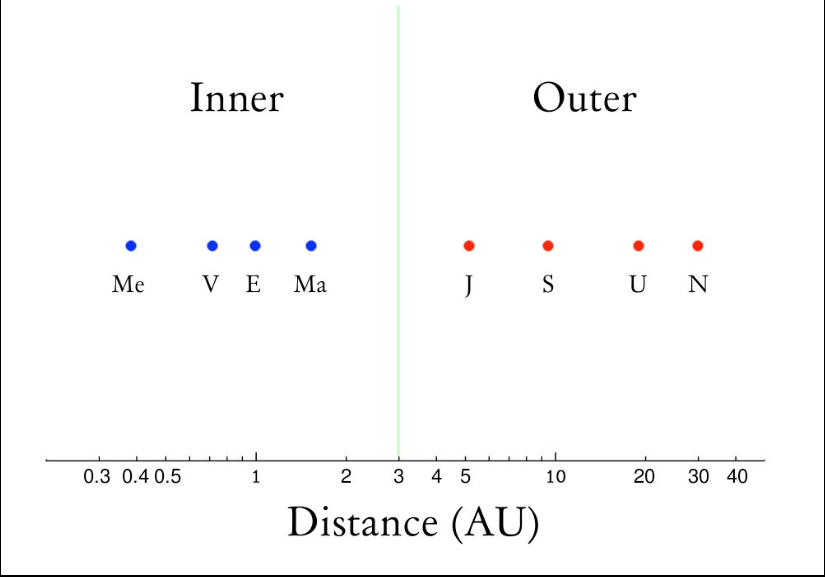
\includegraphics[width=.500\textwidth]{eguzkisistema1}
}
\subfloat[Planeten arteko masa konparaketa.]{
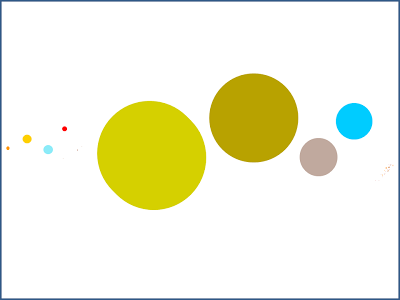
\includegraphics[width=.500\textwidth]{eguzkisistema2}
}
\caption{\small Eguzki-sistema.}
\label{fig:plot1}
\end{figure}    
   
Konputagailuen koma-higikorreko aritmetika ondo ulertzea garrantzitsua da. Zenbaki errealen adierazpen finkoa erabiltzen denez bai zenbakiak memorian gordetzeko, bai hauen arteko kalkulu aritmetikoak egiteko, errore bat egiten dugu. Integrazio luzeetan errore hau propagatzen da eta une batetik aurrera, soluzioen zuzentasuna ezereztatzen da. Ondorioz, integrazioan zehar errore honen monitorizazioa ezagutzea interesgarria da eta integrazio luzeen kasuan, doitasun handian lan egiteko beharra azaltzen zaigu. Gaur egun doitasun altuko aritmetiken erabilera oso garestia da, inplementazioa software bidezkoa delako. Exekuzio denborak onargarriak lortzeko tarteko irtenbidea, inplementazioan doitasun ezberdinak nahastea izango litzateke.       

Sarrera honetan paralelizazioari buruzko ohar bat ematea komeni da. Algoritmo baten kode unitateak paraleloan exekutatzeak badu gainkarga bat eta beraz,  algoritmoaren exekuzioa paralelizazioaz azkartzea lortzeko,  unitate bakoitzaren tamainak esanguratsua izan behar du. Gure Eguzki-sistemaren eredua sinplea da eta logikoa da pentsatzea eredu konplexuagoetan, paralelizazioak abantaila handiagoa erakutsiko duela. Bestalde $N$ gorputzen kopurua handia den problemetan, hauen arteko interakzio kopuru $O(N^2)$ handia kalkulatu behar da eta indar hauen hurbilpena modu eraginkorrean kalkulatzeko metodo ezagunak daude: \textit {tree code} eta \textit {fast multipole method}. Baina gure probleman gorputz kopurua txikia denez, ideia hauek gure eremutik kanpo utzi ditugu. 

\subsection{Overview of the study (structure of the Thesis).}

Gure lanaren abiapuntua Hairer-en IRK metodoaren inplementazioa da. Autoreak IRK puntu-finkoaren inplementazio estandarrean biribiltze errorearen okerreko konportamenduaz jabetu zen eta arazo hau konpontzeko soluzioak proposatu zituen. Lehen urratsa honetan, biribiltze errorearen arazoari soluzio berri bat eman diogu eta gure IRK inplementazioaren oinarriak finkatu: formulazio, koefizienteak, geratze erizpidea,atalen hasierketa \dots.
Gure inplementazioak biribiltze errorea propagazioa optimotik gertu dagoela baieztatzeko, \textit {integratzaile idealaren} soluzioarekin konparatu dugu. Aldi berean, integratzailean biribiltze errorearen estimazioa monitorizatzeko aukera garatu dugu.

Bigarren urratsean, ekuazio sistema ez-lineala ebazteko puntu-finkoaren ordez, Newton sinplifikatuaren metodoa aztertu dugu. Gure ekarpena, Newton sinplifikatua modu eraginkorrean aplikatzeko teknika proposatzea izan da. S-ataletako IRK metodoa eta d-dimentsioko EDA baditugu, Newton sinplifikatuaren metodoren iterazio bakoitzean $sdxsd$ tamainako sistema linealak askatu behar dira. Gure proposamena da, jatorrizko sistema lineala blokeka diagonala den sistema baliokide gisa beridaztea eta matrizearen egitura hau aprobetxatu sistema modu eraginkorrean askatzeko.

Hirugarren urratsean, Eguzki-sitemaren epe luzeko integrazioan arituko gara. Ekarpen handiena, atalen hasieraketa berri bat aplikatzea da alde kepleriarraren fluxuan oinarrituz. IRK metodoak eskeintzen digun malgutasunari esker eta N gorputzetako problema grabitazionalaren ezaugarrietaz baliatuz inplementazio ezberdinak egingo ditugu. Inplementazio hauen eraginkortasuna, egungo integratzaile simplektiko esplizituekin konparatuko ditugu.

Azken urratsean, esperimentalki , eguzki-sistemaren integrazioan  birparametrizazio teknikaren aplikazio sinple bat erakutsiko dugu. Integratzaile sinpletikoak luzeera finkoko urratsa eduki behar du eta zentzu honetan,birparametrizazioa eraginkortasuna hobetzeko beste bide bat da.             
      
\subsection{laburpena}


\part{Background}
\chapter{Zenbakizko Integratzaile Sinplektikoak.}

\section{Sarrera.}

\subsection{Zenbakizko metodoak.}

Ekuazio diferentzial arruntetarako (\emph{ODE}) hasierako baliodun problemen (\emph{IVP}) formulazioa,
\begin{equation}
\label{eq:21}
\dot{\mathbf{y}}(t)=\mathbf{f}(t,\mathbf{y}(t)),\ \ \ \mathbf{y}(t_0)=\mathbf{y_0}, 
\end{equation}
non  $\bf{y}: \mathbb{R} \longrightarrow {\mathbb{R}}^d$ soluzioa, $\bf{y_0} \in \mathbb{R}^d$ hasierako balioa eta $\bf{f}: \ \mathbb{R} \times {\mathbb{R}}^d \ \longrightarrow {\mathbb{R}}^d$ bektore eremua deskribatzen funtzioa dugun ($\dot{\mathbf{y}}$ notazioa erabiliko dugu $d\mathbf{y}/dt$ adierazteko).

\paragraph*{} $t_0$ unetik $t_0+h$ integrazioa,
\begin{equation*}
\mathbf{y}(t_0+h)=\mathbf{y_o}+\int\limits_{t_0}^{t_0+h} \mathbf{f}(t,\mathbf{y}(t)) dt.
\end{equation*}

\paragraph*{}Goiko ekuazio-sistema bektoriala (\ref{eq:21}), ekuazio-sistema modu eskalarrean idatzi daiteke:

\[\dot{y_1}(t)=f_1(t,(y_1(t),y_2(t),\dots,y_d(t)), \ \ y_1(t_0)=y_{1,0}\]
\[\dot{y_2}(t)=f_2(t,(y_1(t),y_2(t),\dots,y_d(t)), \ \ y_2(t_0)=y_{2,0}\]
\[\dots\]
\[\dot{y_d}(t)=f_d(t,(y_1(t),y_2(t),\dots,y_d(t)),  \ \ y_d(t_0)=y_{d,0}\]


\paragraph*{} Metodo analitikoak (funtzio ezagunen araberako soluzio zehatza) eta erdi-analitikoak, ez dira problema askoren soluzioa bilatzeko teknika egokiak. Zenbakizko metodoak, aldiz, modu errazean aplika daitezke eta horregatik, soluzio metodo nagusiena kontsideratzen da. 

\paragraph*{}Zenbakizko metodo baten bidez, $\mathbf{y}(t)$ soluzioaren $\mathbf{y_n} \approx \mathbf{y}(t_n)$ hurbilpena lortuko dugu $t_n=t_{n-1}+h_n$  ($n=1,2,\dots$)  une diskretu ezberdinetarako. Zenbakizko soluzioa urratsez-urrats sekuentzialki eta zehaztutako tarte baterako ($t_0\le t \le t_f$) kalkulatuko dugu. Beraz, lortutako balio  multzoak $(t_o,\mathbf{y_0}),(t_1,\mathbf{y_1}),\dots,(t_f,\mathbf{y_f})$ zenbakizko soluzioa definitzen du.   

\paragraph*{} Nola jakin zenbakizko soluzioa matematika modeloarekiko zuzena dela? Zenbakizko soluzioaren errorea neurtzeko teknika ezberdinak ditugu.           

\paragraph*{} Azkenik argitu beharra dago ekuazio-sistema beti \emph{sistema autonomo} moduan, hau da, denborarekiko independentea idatz daitekeela. Hori horrela izanik, notazioa sinplifikatzeko era honetako sistemak kontsideratuko ditugu,   

\begin{equation}
%\label{eq:31}
\dot{\mathbf{y}}(t)=\mathbf{f}(\mathbf{y}(t)),\ \ \ \mathbf{y}(t_0)=\mathbf{y_0}.
\end{equation}


\paragraph*{}Jarraian zenbakizko metodoen oinarrizko kontzeptuak eta notazioa finkatuko dugu.

\begin{enumerate}

\item Fluxua.

Fase-espazioko edozein $\mathbf{y_0}$ puntuari, $\mathbf{y}(t_0)=\mathbf{y_0}$ hasierako balio duen $\mathbf{y}(t)$ soluzioa asignatzen dion mapping-ari deitzen diogu. Izendatzeko $\varphi_t$ notazioa erabiliko dugu,
\begin{equation*}
\varphi_t(\mathbf{y_0})=\mathbf{y}(t) \ \ \text{baldin} \  \mathbf{y}(t_0)=\mathbf{y_0}
\end{equation*}

\item Zenbakizko diskretizazioa.

$\mathbf{y_{n}},\mathbf{y_{n-1}},\dots ,\mathbf{y_0}$ balioak emanda, $\mathbf{y_{n+1}}\approx \mathbf{y}(t_{n+1})$ soluzioaren hurbilpena kalkulatzeko formulari \emph{zenbakizko fluxua} deritzogu. Honako notazioa erabiliko dugu,
\begin{equation*}
\mathbf{y_{n+1}}=\phi(\mathbf{y_{n+1}},\mathbf{y_{n}},\dots,\mathbf{y_0};h;f).
\end{equation*}

$\phi$ metodoa, $\mathbf{y_{n+1}}$ balioaren menpe ez dagoenean, $\mathbf{y_{n+1}}$ zuzenean kalkula daiteke eta metodoa \emph{esplizitua} dela esaten zaio. Aldiz, $\phi$ metodoa $\mathbf{y_{n+1}}$ menpe dagoenean, $\mathbf{y_{n+1}}$ askatzeko zeharkako bidea erabili behar da (adibidez Newton sinplifikatua edo puntu finkoaren metodoa) eta metodoari \emph{inplizitua} dela esaten zaio.  

\paragraph*{} Adibideak.

Eurler metodo esplizitua.
\begin{equation*}
\label{eq41}
\mathbf{y_{n+1}}=\mathbf{y_n}+h  \ \mathbf{f}(\mathbf{y_n}) 
\end{equation*} 

Eurler metodo inplizitua.
\begin{equation*}
\label{eq41}
\mathbf{y_{n+1}}=\mathbf{y_n}+h  \ \mathbf{f}(\mathbf{y_{n+1}}) 
\end{equation*} 

\item Metodoaren ordena.

\paragraph*{}Definizioa. \textbf{Errore globala}. Zenbakizko soluzioaren $t_0$ hasierako unetik $t_k$ une arteko errore globala $ge(t)$,
\begin{equation*}
ge(t_k)=y_k-y(t_k).
\end{equation*}
  
\paragraph*{} Definizioa. \textbf{$\mathbf{\phi}$ metodoaren ordena}. $h$ urrats luzera finkoko $\phi$ metodoak $p$ ordenekoa dela esaten da, errore globala $ge(t)$  $O(h^{p})$ ordenekoa bada  $h \rightarrow 0$,
\begin{equation*}
y_k-y(t_k)=O(h^{p}), \ \ h \rightarrow 0.
\end{equation*}   

\paragraph*{}Definizioa. \textbf{Errore lokala}. Zenbakizko soluzioaren urrats bakarreko $[t_k,t_{k+1}]$ errore lokala $le(t)$,
\begin{equation*}
le(t_{k+1})=y_{k+1}-y_k(t_{k+1})
\end{equation*}  
non $y_k(t)$, $y(t_k)=y_k$ hasierako balio lokaleko soluzio zehatza den. 

Metodoaren ordena $O(h^p)$ bada, errore lokala $O(h^{p+1})$ da.

\item  Metodo simetrikoak.

\paragraph*{\textbf{Adjoint method}.} Jatorrizko metodoaren alderantzizko eta kontrako denbora $-h$ esleipenari (map), $\phi_h$ metodoaren $\phi_h^{*}$ \emph{adjoint metodoa} esaten zaio.

\begin{equation*}
\phi_h^{*}=\phi_{-h}^{-1}
\end{equation*}

$\phi_h^{*}=\phi_h$  --betetzen denean, metodoa simetrikoa da. 

\end{enumerate}


\subsection{Problema motak.}

\begin{enumerate}

\item Problema kaotikoak. 

Hasierako balio edo parametroen perturbazioekiko, diskretizazio-erroreekiko (trunkatze) edo birbitze erroreekiko esponentzialki sentikorrak diren problemei esaten zaie.

\item Problema stiff.

Irakurri $12.1$ Solution of stiff problems ($555-559$).

Irakurri $13.2.3$ Convergence and consistency and $13.3$ Stiffness and Implicitness (600).

\end{enumerate}


\subsection{Sistema-Hamiltondarrak.}


Ekuazio diferentzial arrunten (EDA) formulazio Hamiltondarra erabili ohi da errealitateko sistemak matematikoki adierazteko. Azpimarratu metodo sinpletikoak sistema Hamiltondar hauen soluzioaren hurbilpena kalkulatzeko zenbakizko metodo bereziki onak ditugula. 

\paragraph*{} $H(\mathbf{p},\mathbf{q})$ funtzio leuna izanik, non  $H: \ {\mathbb{R}}^{d} \ \longrightarrow {\mathbb{R}}$  eta  $(\mathbf{p},\mathbf{q})=(p_1, \dots , p_n,q_1, \dots , q_n)$ ($d=2n$),  dagokion ekuazio diferentzialak era honetan definitzen dira,

\begin{equation}\label{eq:11}
\frac{d}{dt}{p}_j=-\frac{\partial H(\mathbf{p},\mathbf{q})}{\partial q_j}, \ \ \frac{d}{dt}{q}_j=\frac{\partial H(\mathbf{p},\mathbf{q})}{\partial p_j}, \ \ \ \ j=1,\dots,n.
\end{equation} 

Edo notazio laburtua erabiliz,

\begin{equation}
\dot{\mathbf{y}}=J^{-1}\triangledown H(\mathbf{y}),\ \ 
y=\left(\begin{array}{c}
  p \\
  q \\
  \end{array}\right), \ \
J=\left(\begin{array}{cc}
  \ 0 & \ I \\
   -I & \ 0 \\
\end{array}\right),  
\end{equation}

\paragraph*{}$\mathbf{p}$ eta $\mathbf{q}$ bektoreen $n$ dimentsioa sistemaren \emph{askatasun maila} deritzo. $H(\mathbf{p},\mathbf{q})$ funtzioaren balioa integrazioan zehar konstante mantentzen da.

\subsubsection*{Adibidea.} Penduluaren problemaren (masa $m=1$, $l=1$ luzerako makila eta $g=1$ grabitazioa) askatasun bakarreko sistema Hamiltondarra,

\begin{equation*}
H(p,q)=\frac{1}{2} p^2- cos q.
\end{equation*}

Ekuazio diferentzialak,
\begin{equation*}
\dot{p}= -sin q, \ \ \dot{q}=p.
\end{equation*}

\begin{figure}[h]
\centering
\subfloat[Pendulua.]{
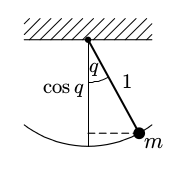
\includegraphics[width=.250\textwidth]{SinglePendulum}
}
\caption{ \small Pendulua.}
\label{fig:pendulua}
\end{figure}

\subsubsection*{Hamiltondar banagarriak.}

Hamiltondar banagarriak egitura bereziko sistema Hamiltondarrak ditugu. Sistema-mekanikoak era honetako Hamiltondarra dute $H(\mathbf{p},\mathbf{q})=T(\mathbf{p})+U(\mathbf{q})$.

Horien artean, \emph{bigarren ordeneko} ekuazio diferentzialak aipatu behar ditugu, zeintzuk Hamiltondar banagarri kasu partikularra bat diren,  

\begin{equation*}
H(\mathbf{p},\mathbf{q})=\frac{1}{2}\mathbf{p}^T\mathbf{p} +U(\mathbf{q}).
\end{equation*}

Beraz, dagokien ekuazio diferentzialak,
\begin{equation*}
\dot{\mathbf{p}}=-\frac{\partial U(\mathbf{q})}{\partial \mathbf{q}}, \ \ \dot{\mathbf{q}}=\mathbf{p}. 
\end{equation*}

\subsubsection*{Adibidea.}
\emph{Bi-gorputzen problema} edo \emph{Kepler problema}. Planoan elkar erakartzen diren bi gorputzen (planeta eta eguzkia) mugimendua kalkulatzeko, horietako gorputz baten kokapena koordenatu sistemaren jatorria kontsideratuko dugu eta beste gorputzaren kokapenaren koordenatuak $\mathbf{q}=(q_1,q_2)$ aukeratuko ditugu. Normalizatutako Newton legearen araberako ekuazio diferentzialak,  

\begin{equation}
\dot{p}_1= -\frac{q_1}{(q_1^2+q_2^2)^{3/2}}, \ \, \dot{p}_2= -\frac{q_2}{(q_1^2+q_2^2)^{3/2}}.
\end{equation}
  
\begin{equation}
\dot{q}_i=p_i, \ \ i=1,2.
\end{equation}

Baliokide den sistema Hamiltondarra,
\begin{equation}
H(p_1,p_2,q_1,q_2)=\frac{1}{2}(p_1^2+p_2^2)-\frac{1}{\sqrt{q_1^2+q_2^2}}.
\end{equation}

\paragraph*{} Planetaren mugimendua orbita eliptiko bat da. Honako hasierako balioei dagokien soluzioa,
\begin{equation*}
q_1(0)=1-e, \ q_2(0)=0, \ p_1(0)=0, \ p_2(0)=\sqrt{ \frac{1+e}{1-e}}, 
\end{equation*}
$e$ ezentrizidade ($0\le e < 1$) duen elipsea da, eta $P=2\pi$ periododuna. 
 
\subsubsection*{Hamiltondar perturbatuak.}

Hamiltondar perturbatuak, honako egitura duten,

\begin{equation*}
H=H_A+\epsilon H_B \ \ (|H_B|\ll |H_A|),
\end{equation*}

sistemak ditugu. Adibidez Eguzki sistemaren probleman, Hamiltondarra modu honetan idatzi daiteke $H=H_k+H_I$, non alde nagusia $H_K$ planeta bakoitzaren eguzki inguruko mugimendu kepleriarra den eta $H_I$ aldiz, planeten arteko interakzioek eragiten duten perturbazio txikia.   

Eguzki-sistemaren kasuan, \emph{Jakobi} koordenatuak erabiliz Hamiltondarra $H(\mathbf{p},\mathbf{q})=H_K(\mathbf{p},\mathbf{q})+H_I(\mathbf{q})$ moduan banatzen da, non $H_K(\mathbf{p},\mathbf{q})$ Kepler problema independenteak eta $H_I(\mathbf{q})$ integratu daitezkeen. Beste aukera, koordenatu \emph{Heliozentrikoak} erabiliz $H(\mathbf{p},\mathbf{q})=H_K(\mathbf{p},\mathbf{q})+H_I(\mathbf{p},\mathbf{q})$ moduan banatzen da, non $H_I(\mathbf{p},\mathbf{q})$ ezin daitekeen zuzenean integratu.

\section{Metodo sinplektikoak.}

\paragraph*{} Urrats luzera. Metodo gehienak eraginkorrak izateko, errore estimazio baten arabera integrazioan zehar urrats luzera egokitzen dute. Integratzaile sinplektikoetan, urrats luzeera finkoa erabili behar da metodoaren propietateak ez galtzeko.  

\paragraph{\textbf{Implicit midpoint}.}

\begin{equation*}
p_{n+1}=p_n-h \triangledown_q H(\frac{p_{n+1}+p_n}{2},\frac{q_{n+1}+q_n}{2})
\end{equation*}

\begin{equation*}
q_{n+1}=q_n+h \triangledown_p H(\frac{p_{n+1}+p_n}{2},\frac{q_{n+1}+q_n}{2})
\end{equation*}

\paragraph*{\textbf{Störmer-Verlet  metodoa}.}
$p=2$ ordeneko metodo sinplektikoa eta simetrikoa dugu.

\[p_{\frac{n+1}{2}}=p_n-\frac{h}{2} \triangledown_q H(p_{\frac{n+1}{2}},q_n) \]
\begin{equation}
q_{n+1}=q_n+\frac{h}{2} \big(\triangledown_p H(p_{\frac{n+1}{2}},q_n)+ \triangledown_p H(p_{\frac{n+1}{2}},q_{n+1}) \big)
\end{equation}
\[p_{n+1}=p_{\frac{n+1}{2}}-\frac{h}{2} \triangledown_q H(p_{\frac{n+1}{2}},q_{n+1}) \]

edo

\[q_{\frac{n+1}{2}}=q_n+\frac{h}{2} \triangledown_p H(p_n,q_{\frac{n+1}{2}}) \]
\begin{equation}
p_{n+1}=p_n-\frac{h}{2} \big(\triangledown_q H(p_n,q_{\frac{n+1}{2}})+ \triangledown_q H(p_{n+1},q_{\frac{n+1}{2}}) \big)
\end{equation}
\[q_{n+1}=q_{\frac{n+1}{2}}+\frac{h}{2} \triangledown_p H(p_{n+1},q_{\frac{n+1}{2}}) \]


\paragraph*{}Bigarren ordeneko ekuazio diferentziala ditugunean metodoa esplizitua da eta modu honetan labur daiteke,

\[p_{{n+1}/{2}}=p_n+\frac{h}{2} f(q_n)\]
\begin{equation}
q_{n+1}=q_n+h p_{{n+1}/{2}}
\end{equation}
\[p_{n+1}=p_{{n+1}/{2}}+\frac{h}{2}f(q_{n+1})\]

edo

\[q_{{n+1}/{2}}=q_n+\frac{h}{2} p_n\]
\begin{equation}
p_{n+1}=p_n+h f(q_{{n+1}/{2}})
\end{equation}
\[q_{n+1}=q_{{n+1}/{2}}+\frac{h}{2} p_{n+1}\]

\section{Gauss metodoak.}

\subsection{Runge-Kutta metodoak.}

Runge-Kutta metodoak, urrats bakarreko ekuazio diferentzial arrunten zenbakizko integratzaileak dira.  $b_{i}$, $a_{ij}$ eta $c_i=\sum\limits_{i=0}^{s} a_{ij} \ (1 \leq i,j \leq s)$ koefiziente errealek s-ataleko Runge-Kutta metodoa definitzen dute . \emph{Butcher} izeneko taulan moduan laburtu ohi dira koefiziente hauek, 

\begin{equation}
\begin{array}{c|c}
  \bf{c} & \bf{A} \\
  \hline
         &  \bf{b}^T\\
\end{array}, \ \ \ \ \ \ \ \ \ \ \ \
\begin{array}{c|cccc}
  \ c_1 &  a_{11} & a_{12} & \dots & a_{1s}\\
  \ c_2 &  a_{21} & a_{22} & \dots &a_{2s}\\
  \ \vdots & \vdots & \ddots & & \vdots \\
  \ c_s & a_{s1} & a_{s2} & \dots & a_{ss}\\
  \hline
  \  & b_{1} & b_{2} & \dots & b_{s}\\
\end{array}
\end{equation}

\paragraph*{} Hasierako baliodun problema (\ref{eq:21}) baten $\mathbf{y}(t)$ soluzioaren $\mathbf{y}_n \approx \mathbf{y}(t_n)$ hurbilpena era honetan kalkulatzen da,

\begin{equation}  
\mathbf{y}_{n+1}=\mathbf{y}_n+h\sum^s_{i=1}{b_i \ \mathbf{f}(\mathbf{Y}_{n,i})\ \ },\
\end{equation} 

non $\mathbf{Y}_{n,i}$ atalak era honetan definitzen diren,
\begin{equation}
\mathbf{Y}_{n,i}=\mathbf{y}_n+\ h\ \sum^s_{j=1}{a_{ij}\ \mathbf{f}(\mathbf{Y}_{n,j})}\ \ \ \ \ i=1 ,\dots, s.\
\end{equation} 

\subsubsection*{Metodo esplizituak (ERK) eta inplizituak (IRK).}
Bi mota nagusi bereizi ditzakegu: esplizituak (\emph {ERK}) non $\forall i\ge j, \ a_{ij}=0 $ eta inplizituak (\emph {IRK}) non $\exists i \ge j \ , a_{ij} \ne 0$ . \emph{ERK} metodoak problema Nonstiff-etarako eraginkorrak kontsideratzen dira eta \emph{IRK} metodoak ordea, problema Stiff-etarako.

\paragraph*{} Adibideak: ERK lau-ataletako metodo klasikoa (ezkerrekoa) and Implicit Midpoint method (eskuindekoa). 
\begin{equation}
\begin{array}{c|cccc}
  \ 0   &    &    &     &      \\
  \ 1/2 & 1/2 &   &     &      \\
  \ 1/2 & 0   & 1/2  &  &      \\
  \ 1   & 0   & 0    &  1   &   \\
  \hline
  \     & 1/6 & 2/6  &  2/6 & 1/6 \\
\end{array}, \ \ \ \ \ \ \ \ \ \ \ \
\begin{array}{c|c}
  \ 1/2 &  1/2\\
  \hline
  \     & 1 \\
\end{array} \\
\end{equation}

\paragraph*{}\emph{ERK} lau-ataletako  metodo klasikoa $p=4$ ordeneko dugu. Orden altuko \emph{ERK} metodoak aurkitzea konplexua da,  betearazi behar diren baldintza kopuru esponentzialki hazten baitira. Orden altuko \emph (ERK) metodo hauek aurkitu dira: $p=8$ ordeneko metodoa $s=11$ atalekin, $p=10$ ordeneko metodoa $s=17$ atalekin eta  $p=12$ ordeneko metodoa $s=25$ atalekin. 

\paragraph*{} \emph{IRK} metodoak \emph{ERK} metodoak baino modu errazagoan eraiki daitezke.  \emph{Butcher sinplifikazio baldintzen} \cite{Butcher2008} arabera definitzen dira,

\begin{equation*}
B(p): \ \ \ \sum\limits_{i=1}^{s} b_ic_i^{q-1}=\frac{1}{q}, \ \ q=1,\dots,p.
\end{equation*}

\begin{equation*}
C(\eta): \ \ \ \sum\limits_{j=1}^{s} a_{ij}c_j^{q-1}=\frac{c_i^q}{q}, \ \ i=1,\dots,s, \ q=1,\dots,\eta.
\end{equation*}

\begin{equation*}
D(\zeta):  \ \ \ \sum\limits_{i=1}^{s}  b_i c_i^{q-1}  a_{ij}  = \frac{b_j}{q} (1-c_j^q),  \ j=1,\dots,s, \ q=1,\dots,\zeta.
\end{equation*}

\begin{table}{htb}
\caption{Runge-Kutta metodo inplizituak.}
\label{tab:21}       % Give a unique label
\begin{tabular}{ c c c c c } 
 \hline
 Metodoa          &  Baldintzak             &                        &                 & Ordena \\
 \hline
 Gauss            &  $B(2s)$                & $C(s)$                 & $D(s)$          & $2s$    \\
 \hline
 Radau IA         &  $B(2s-1)$              & $C(s-1)$               & $D(s)$          & $2s-1$  \\
 \hline 
 Radau IA         &  $B(2s-1)$              & $C(s)$                 & $D(s-1)$        & $2s-1$  \\
 \hline 
 Lobatto IIIA     &  $B(2s-2)$              & $C(s)$                 & $D(s-2)$        & $2s-2$  \\
 \hline
 Lobatto IIIB     &  $B(2s-2)$              & $C(s-2)$               & $D(s)$          & $2s-2$  \\
 \hline 
 Lobatto IIIC     &  $B(2s-2)$              & $C(s-1)$               & $D(s-1)$        & $2s-2$  \\
  \hline
 \end{tabular}
\end{table}

\paragraph*{}Aurreko taulan (Taula \ref{tab:21}) \emph{IRK} metodo ezagunenak laburtu ditugu. Gauss metodoa s-ataletako IRK metodoen artean $p=2s$ ordena duen metodo bakarra dugu. Gauss metodoa sinplektikoa eta simetrikoa da.

\begin{enumerate}
\item{Sinplektizidade baldintza} \cite{JMSanz-Serna1994}.
\begin{equation} \label{eq:1}
b_{i}a_{ij}+b_{j}a_{ji}-b_{i}b_{j}=0, \ \ 1 \leqslant i,j \leqslant s
\end{equation}
%\cite{Sanz-Serna1992}.
 
\item{Koefiziente simetrikoak}.
 \begin{equation} \label {eq:2}
 b_{i} = b_{(s-i+1)} ,\ \  i=1,2,\dots \lceil s/2\rceil
 \end{equation} 
  \begin{equation} \label{eq:3}
 c_{(s-i+1)}= 1-c_{i}, \ \  i=1,2,\dots \lceil s/2\rceil
 \end{equation} 
 
 \begin{figure}[h]
 \centering
 \subfloat[Kolokazio metodoen simetria.]{
 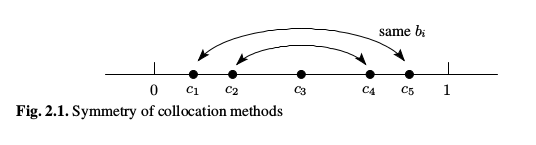
\includegraphics[width=.850\textwidth]{SymmetryCollocation}
 }
 \caption{ \small Kolokazio metodoen simetria.}
 \label{fig:pendulua}
 \end{figure}
  
\end{enumerate}

\paragraph{\textbf{Adibidea}.} $s=1$, $s=2$ eta $s=3$ ataletako Gauss metodoak.
\begin{equation*}
\begin{array}{c|c}
  \frac{1}{2} & \ \frac{1}{2} \\
  \hline
   & 1 \\
\end{array} \ \ \ ,  \ \ \ \ \ \ \ \ \
\begin{array}{c|c c}
  \frac{1}{2}-\frac{\sqrt{3}}{6} & \ \frac{1}{4} & \ \frac{1}{4}-\frac{\sqrt{3}}{6} \\
  \frac{1}{2}+\frac{\sqrt{3}}{6} & \ \frac{1}{4}+\frac{\sqrt{3}}{6} & \ \frac{1}{4} \\
  \hline
         &  \frac{1}{2} & \ \frac{1}{2} \\
\end{array}
\end{equation*}

\begin{equation*}
\begin{array}{c|c c c}
  \frac{1}{2}-\frac{\sqrt{15}}{10} & \ \frac{5}{36} & \ \frac{2}{9}-\frac{\sqrt{15}}{15} & \ \frac{5}{36}-\frac{\sqrt{15}}{30} \\
  \frac{1}{2}   & \ \frac{5}{36}+\frac{\sqrt{15}}{24} & \ \frac{2}{9} & \ \frac{5}{36}-\frac{\sqrt{15}}{24} \\
  \frac{1}{2}+\frac{\sqrt{15}}{10}   & \ \frac{5}{36}+\frac{\sqrt{15}}{30} & \ \frac{2}{9}+\frac{\sqrt{15}}{15} & \ \frac{5}{36} \\
  \hline
  & \frac{5}{18} & \ \frac{4}{9} & \ \frac{5}{18}
\end{array}
\end{equation*}

\paragraph*{}\emph{IRK} metodoetan, erronka handiena ekuazio-sistema ez-linealaren zenbakizko soluzio eraginkorra exekutatzea da. Nonstiff problemetarako, atalen hasieraketa ($Y_i^{[0]}$) egoki bat duen puntu-finkoko iterazioa erabil daiteke. Stiff problemetarako, puntu-finkoa iterazioak urrats tamaina txikiegia izatea behartuko luke eta ondorioz, Newton sinplifikatua erabili ohi da.         

\subsection*{IRK algoritmo orokorra.}


\begin{algorithm}[H]
 \BlankLine
  \For{$n\leftarrow 1$ \KwTo $endstep$}
  {
   \BlankLine
   Hasieratu  $Y_{i,n}^{[0]} \ \ , \ \ i=1,\dots,s $\;
    \BlankLine
   \While{ (konbergentzia lortu)}
   {
    \BlankLine 
    $F_{n,i}=f(Y_{n,i}) \ \ , \ \  i=1,\dots,s$\;
    $Y_{n,i}=y_{n-1}+ h \ \sum\limits_{j=1}^{s} a_{ij} F_{n,j}  \ \ , \ \  i=1,\dots,s$\;  
   }
   \BlankLine
    $y_{n}=y_{n-1}+ h \ \sum\limits_{i=1}^{s} b_i F_{n,i} $\;
   \BlankLine
 }
 \caption{Main Algorithm}
\end{algorithm}

\paragraph*{}Algoritmo nagusiko agindu bakoitzari ohar moduko egingo diogu, IRK metodoaren hainbat zehaztapen emateko helburuarekin.
\begin{enumerate}
\item Hasieratu  $Y_{i,n}^{[0]}$.

Atalen hasieraketa egokia definitu behar da. Aukera sinpleena $Y_{i,n}^{[0]}=y_{n-1}$ hasieratzea da baina aurreko urratseko informazioa erabiliz hurbilketa hobea lortu daiteke. Aurreko urratseko atalen polinomio interpolatzailearen bidezko hasieraketa era honetan adierazi dezakegu  $Y_{i,n}^{[0]}=g(Y_{i,n-1}) \ , \ i=1, \dots, s$.      

\item $F_{n,i}=f(Y_{n,i})$.

Atal bakoitzarentzat ekuazio diferentzialaren balioztapena independentea da eta modu paraleloan exekutatu daiteke.

\item   $Y_{n,i}=y_{n-1}+ h \ \sum\limits_{i=1}^{s} a_{ij} F_{n,j}  \ \ , \ \  i=1,\dots,s$.

Ekuazio-sistema ez lineala metodo iteratibo bat erabiliz askatu behar da. Metodo hau, Puntu-finkoaren metodoa edo Newton  sinplifikatuaren metodoa izan daiteke.  

\begin{enumerate}

\item Puntu-finkoko iterazioa.

\begin{algorithm}[H]
  \For{ (k=1,2,\dots)}
  {
   $Y_{i}^{[k]}=y_{n-1}+ h \ \sum\limits_{j=1}^{s} a_{ij} f(Y_i^{[k-1]}) $\; 
  }
 \caption{Main Algorithm}
\end{algorithm}


\item Newton sinplfifikatua.

Ekuazio-linealaren matrizea $M= I_s \otimes I_d -hA \otimes J, J=f'(y_n)$\$ definitzen dugu. Newton sinplifikatua puntu-finkoko iterazioa baino garestiagoa da, jakobiarra eta $M$ matrizearen \emph{LU-deskonposaketa} kalkulatu behar baititugu.  

\begin{algorithm}[H]
  $J=f'(y_n)$\;
  $M= I_s \otimes I_d -hA \otimes J$\;
  \For{ (k=1,2,\dots)}
  {
   $M\triangle Y^{[k-1]}=-F(Y^{k-1})$\;
   $Y^{[k]}=Y^{[k-1]}+\triangle Y^{[k-1]}$\; 
  }
 \caption{Main Algorithm}
\end{algorithm}


\end{enumerate}


\item $y_{n}=y_{n-1}+ h \ \sum\limits_{i=1}^{s} b_i F_{n,i} $\;

Integrazio luzeak direnean, urrats asko ematen dira eta koma higikorreko aritmetika dela eta, doitasun galera ekiditeko batura konpensatu teknika erabili ohi da.


\end{enumerate} 

\subsubsection*{Bigarren ordeneko ekuazio diferentzialak.}

Era honetako ekuazio diferentzialak ,

\begin{equation*}
\dot{u}=f(v), \ \ \dot{v}=g(u),
\end{equation*}

garrantzitsuak dira. Esaterako, bigarren ordeneko ekuazio diferentziala $\ddot{y}=f(y)$ eta Hamiltondar banagarriak $H(q,p)=T(p)+U(q)$ hauen kasu partikularra ditugu.

Runge-Kutta metodoaren ekuazioak era honetan bilakatzen dira,

\begin{equation*}
U_{i,n}=u_n+ \sum\limits_{i=1}^{s} a_{ij} f(V_{i,n})
\end{equation*}

\begin{equation*}
V_{i,n}=v_n+ \sum\limits_{i=1}^{s} a_{ij} g(U_{i,n})
\end{equation*}

Kasu honetan Gauss-Seidel iterazioa, puntu-finkoaren iterazio estandarra baino hobea da,

\begin{algorithm}[H]
  \For{ (k=1,2,\dots)}
  {
   $U_{i}^{[k+1]}=u_{n}+ h \ \sum\limits_{j=1}^{s} a_{ij} f(V_i^{[k]}) $\; 
   $V_{i}^{[k]}=v_{n}+ h \ \sum\limits_{j=1}^{s} a_{ij} g(U_i^{[k+1]}) $\; 
  }
 \caption{Main Algorithm}
\end{algorithm}
 
\paragraph*{}Bigarren ordeneko ekuazio diferentzialak ditugunean,
\begin{equation*}
\dot{u}=f(v), \ \ \dot{v}=u,
\end{equation*}

Gauss-Seidel iterazioa honakoa dugu,

\begin{algorithm}[H]
  \For{ (k=1,2,\dots)}
  {
   $V_{i}^{[k+1]}=v_{n}+h c_i v_{n}+ h^2 \ \sum\limits_{j=1}^{s} \tilde{a}_{ij} f(V_i^{[k]}) $\;  
  }
 \caption{Main Algorithm}
\end{algorithm} 


 

\subsection{Kolokazio metodoak.}

Kolokazio metodoak ekuazio diferentzialen zenbakizko soluzioa azaltzeko beste modu bat dira. Gauss metodoak kolokazio metodoak ditugu eta hauen abantaila da, zenbakizko soluzioa diskretizazio puntuetan ez ezik, polinomio interpolatzaile batek modu jarraian emandako soluzioa adierazten duela. Honako definizioa emango dugu,

\begin{definizioa}
$c_1,c_2,\dots,c_s \ \ (0\leq c_i \leq 1)$ zenbaki errealak izanik, $s$-mailako $u(t)$   kolokazio polinomioak honakoa betetzen du,

\[u(t_0)=y_0 ,\]
\[\dot{u}(t_0+c_ih)=f(t_0+c_i h, u(t_0+c_i h)), \ \ i=1,\dots,s.\] 


Orduan soluzioa $y_1=u(t_0+h)\approx y(t_0+h)$ da..
\end{definizioa}

\begin{teorema}
\textbf{Theorem 1.4 (Guillou and Soule 1969, Wright 1970).}
Kolokazio metodoaren definizioa eta jarraian emandako moduan kalkulatutako koefizienteko s-ataleko Runge-Kutta metodoa baliokideak dira.

\begin{equation}
a_{ij}=\int_{0}^{c_i} l_j(\tau) \ d\tau, \ \ b_i=\int_{0}^{1} l_i(\tau) \ d\tau
\end{equation}

non $l_i(\tau)$ Lagrangiar polinomioa dugu $l_i(\tau)=\prod_{l\neq i} \frac{(\tau-c_l)}{(c_i-c_l)}$.
\end{teorema}

\paragraph{\textbf{Definizioa}.} Gauss metodoak $c_i$ ($1 \leq i \leq s)$ koefizienteak "sth shifted Legendre" polinomioaren zeroak aukeratuz,

\begin{equation*}
\frac{d^s}{dx^s} \big(x^s(x-1)^s \big),
\end{equation*} 

Nodo hauetan oinarritutako Runge-Kutta metodoa $p=2s$ ordena du.

\begin{figure}[h]
\centering
\subfloat[kolokazio metodoak.]{
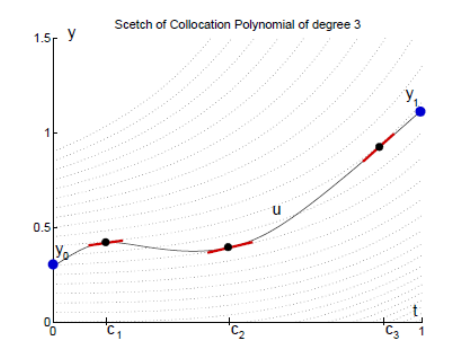
\includegraphics[width=.450\textwidth]{KolokazioMetodoa}
}
\caption{ \small kolokazio metodoak.}
\label{fig:kolokazio metodoak}
\end{figure}


\paragraph*{} Gauss metodoaren koefizienteak kalkulatzeko bi aukera ditugu. Lehen aukera,  \emph{Mathematicak} NDSolve paketean inplementatuta dagoen koefizienteak kalkulatzeko funtzioa: ImplicitRungeKuttaGaussCoefficients[]. Bigarren aukera, guk koefizienteak kalkulatzeko garatutako funtzioa erabiltzea.  

\begin{lstlisting} [language=Mathematica]

GaussCoefficients[s_Integer, doi_, a_Symbol, b_Symbol, c_Symbol] :=
    Module[{f, g, ff, glist, B, A},
 
         Do[c[i] = N[(Root[LegendreP[s, #] &, i] + 1)/2, doi] // Simplify, {i, s}
           ];
         ff = Collect[InterpolatingPolynomial
                     [Table[{c[i], f[i]}, {i, s}], x], f[_]];
         glist = Table[g[i] = Collect[ff, f[_],
                                      Simplify[\!\(\*SubsuperscriptBox[\(\[Integral]\), \(0\), \(c[
          i]\)]\(#1 \[DifferentialD]x\)\)] &], {i, 1, s}];
               yy = Collect[ff, f[_], Simplify[\!\(
\*SubsuperscriptBox[\(\[Integral]\), \(0\), \(1\)]\(#1 \
\[DifferentialD]x\)\)] &];
                B = Table[b[i] = \!\(
\*SubscriptBox[\(\[PartialD]\), \(f[i]\)]yy\), {i, 1, s}];
               
 A = Table[a[i, j] = D[g[i], f[j]], {i, 1, s}, {j, 1, s}];
         {Array[c, s], B, A}
 ]

\end{lstlisting}


\section{Konposizio metodoak.}

\subsection{Sarrera.}

Konposizio metodoak, oinarrizko metodo bat edo gehiago konposatuz eraikitako zenbakizko integrazio metodoak dira.  Oinarrizko metodoekin segidan exekutatutako azpi-urrats kopuru batek, konposizio metodoaren integrazioaren urrats bat osatzen du. Helburua orden baxuko metodo batetik abiatuta, orden altuko metodoa eraikitzea da; konposizio metodoak automatikoki konposatutako metodoaren propietateak (simetri, sinplektikoa,\dots) jasotzen ditu. 

\paragraph*{\textbf{Definizioa orokorra}.}
$\phi_h$ oinarrizko metodoa eta $\gamma_1,\dots,\gamma_s$ zenbaki errealak emanik, urrats luzera hauen $\gamma_1 h,\gamma_2 h,\dots,\gamma_s h$ konposaketari dagokion konposizio metodoa,
\begin{equation}
\Psi_h=\phi_{\gamma_s h} \circ \dots \circ \phi_{\gamma_{1 h}}.
\end{equation}

\paragraph*{\textbf{Teorema}.}
Demagun $\phi_h$ urrats bakarreko eta $p$ ordeneko metodoa. Konposizio metodoa gutxienez $p+1$ ordeneko izango da baldin,
\[\gamma_1+\dots+\gamma_s=1,\] 
\begin{equation}
\gamma_1^{p+1}+\dots+\gamma_s^{p+1}=0.
\end{equation}

\paragraph*{\textbf{Algoritmoa}.}
Konposizio metodoen algoritmo orokorra honakoa izango litzateke:

\begin{algorithm}[H]
 \BlankLine
  \For{$n\leftarrow 1$ \KwTo $endstep$}
  {
   \BlankLine
    $Y_{0,n}=y_{n-1} $\;
    \BlankLine
   \For{i=1,2,...,s}
   {
    \BlankLine 
    $Y_{i,n}=\phi_{\gamma_i h}(Y_{i-1,n})$\;
   }
   \BlankLine
    $y_{n}=Y_{s,n}$\;
   \BlankLine
 }
 \caption{Konposizio metodoak.}
\end{algorithm}
 
\paragraph*{Oharrak.}
Konposizio metodoei buruzko hainbat ohar azpimarratuko ditugu:
\begin{enumerate}
\item{Esplizitua.}

Konposizio metodo hauek esplizituak dira. Metodo hauetan ez da ekuazio sistemarik askatu behar, eta kalkuluak azkarrak dira. 

\item{Sekuentziala.}

Urrats bakoitzaren kalkuluak modu sekuentzialean egin behar ditugu.

\item{Memoria gutxi.}

Ez da tarteko baliorik gorde behar eta datu-egitura berezirik memorian gorde behar.   

\item{Oinarrizko metodoa: Störmer-Verlet.}

Bigarren ordeneko ekuazio diferentzialak ditugunean, Störmer-Verlet integratzailean oinarritzen diren konposizio metodoekin urrats bakoitzean $s$ ekuazio diferentzialaren balioztapena egin behar ditugu.

\end{enumerate}


\paragraph*{} Konposizio metodo eraginkorra $s$-atal gutxirekin, $p$ orden altuko metodoa dugu. Sofronio eta Spalettaren ($2004$), $s=35$ eta $p=10$ ordeneko metodoa \cite{Sofroniou2005}, orain arteko lortutako orden altueneko konposizio metodo eraginkorrena kontsideratu daiteke. \emph{IRK} metodoa konposizio metodo honekin alderatuko dugu eta beraz, jarraian modu laburrean konposizio metodo hau azalduko dugu.     

\subsection{CO1035: $10$ ordeneko konposizio metodoa.}

Konposizio metodo simetrikoa da. Oinarrizko metodoa simetrikoa eta $p=2$ dela baliatuz eraikitako metodoa da. 

\begin{table}
\caption[C01035 konposizio metodoa.] 
{\small{10 ordeneko metodoa konposizio metodoa (CO1035).}}
\label{tab:31}       % Give a unique label
\begin{tabular}{ c c } 
 \hline
 Koefiziente         &  Balioa \\
 \hline
 $\gamma_1=\gamma_{35}$ & 0.07879572252168641926390768 \\
 $\gamma_2=\gamma_{34}$ & 0.31309610341510852776481247 \\ 
 $\gamma_3=\gamma_{33}$ & 0.02791838323507806610952027 \\
 $\gamma_4=\gamma_{32}$ &-0.22959284159390709415121340 \\ 
 $\gamma_5=\gamma_{31}$ & 0.13096206107716486317465686 \\ 
 $\gamma_6=\gamma_{30}$ & -0.26973340565451071434460973 \\ 
 $\gamma_7=\gamma_{29}$ & 0.07497334315589143566613711 \\ 
 $\gamma_8=\gamma_{28}$ & 0.11199342399981020488957508 \\ 
 $\gamma_9=\gamma_{27}$ & 0.36613344954622675119314812 \\ 
 $\gamma_{10}=\gamma_{26}$ & -0.39910563013603589787862981 \\ 
 $\gamma_{11}=\gamma_{25}$ & 0.10308739852747107731580277 \\
 $\gamma_{12}=\gamma_{24}$ & 0.41143087395589023782070412 \\ 
 $\gamma_{13}=\gamma_{23}$ & -0.00486636058313526176219566 \\ 
 $\gamma_{14}=\gamma_{22}$ & -0.39203335370863990644808194 \\ 
 $\gamma_{15}=\gamma_{21}$ & 0.05194250296244964703718290 \\ 
 $\gamma_{16}=\gamma_{20}$ & 0.05066509075992449633587434 \\ 
 $\gamma_{17}=\gamma_{19}$ & 0.04967437063972987905456880 \\ 
 $\gamma_{18}$ & 0.04931773575959453791768001 \\ 
  \hline
 \end{tabular}
\end{table}


\paragraph*{\textbf{Gure inplementazioa.}} Gure abiapuntua Haireren konposizio metodoaren Fortran kodea izan da. Konposizio metodoaren azalpenak liburuko \cite{Hairer2006}  \emph{II.4} eta \emph{V.3} ataletan ematen ditu. \emph{GNI-Comp} izeneko kodea eskuragarri dago \cite{HairerGniComp} helbidean. Kodearen C-lengoaiako bertsioa garatu dugu.

\paragraph*{}$\phi_h$ metodoa $p=2$ ordenekoa eta simetrikoa izanik, era honetako konposizioak aurkitu dira,
\begin{equation}
\Psi_h=\phi_{\gamma_s h} \circ \phi_{\gamma_s-1 h} \circ \dots \circ \phi_{\gamma_{2 h}} \circ \phi_{\gamma_{1 h}} 
\end{equation}
non $\gamma_s=\gamma_1, \gamma_{s-1}=\gamma_2,\dots$ 


\paragraph*{\textbf{Koefizienteak}.}

Konposizio metodoaren oinarrizko metodoa \emph{Stömer-Verlet}  $\phi_h=\varphi_{h/2}^{1} \circ \varphi_{h}^{2} \circ \varphi_{h/2}^{1}$  dugula kontutan hartuta,

\begin{equation*}
\Psi_h=(\varphi_{h \gamma_s/2}^{1} \circ \varphi_{h \gamma_s}^{2} \circ \varphi_{h \gamma_s/2}^{1}) \circ \dots 
       \circ
       (\varphi_{h \gamma_2/2}^{1} \circ \varphi_{h \gamma_2}^{2} \circ \varphi_{h \gamma_2/2}^{1}) 
       \circ
       (\varphi_{h \gamma_1/2}^{1} \circ \varphi_{h \gamma_1}^{2} \circ \varphi_{h \gamma_1/2}^{1})  
\end{equation*}

\paragraph*{}Beraz jarraian dauden $\varphi^1$ fluxuak elkartuz,

\begin{equation*}
\Psi_h=\varphi_{h a_{s+1}}^{1} \circ \varphi_{h b_s}^{2} \circ \dots 
       \circ
       \varphi_{h a_3} \circ \varphi_{h b_2}^{2} 
       \circ
       \varphi_{h a_2}^{1} \circ \varphi_{h b_1}^{2} \circ \varphi_{h a_1}^{1}  
\end{equation*}

non $a_1=a_{s+1}=\gamma_1/2$, $b_i=\gamma_i$, $a_k=(\gamma_k+\gamma_{k-1})/2$, $i=1,\dots,s$ eta $k=2,\dots,s$.

\paragraph*{}Tarteko urratsetan, lehen atala $\varphi_{h a_1}^{1}$ eta azkena $\varphi_{h a_1}^{1}$ bakar batean elkar daitezke, 

\begin{equation*}
\Psi_h=\varphi_{h 2 a_{s+1}}^{1} \circ \varphi_{h b_s}^{2} \circ \dots 
       \circ
       \varphi_{h a_3} \circ \varphi_{h b_2}^{2} 
       \circ
       \varphi_{h a_2}^{1} \circ \varphi_{h b_1}^{2}.
\end{equation*}

\section{Splitting metodoak.}

\subsection{Sarrera.}

\emph{Splitting metodoak}, bektore eremua $f: \mathbb{R}^d \rightarrow \mathbb{R}^d$ sistema osoa integratzeko baino errazagoa diren azpiproblemetan, $f^{[i]}$ ($f=\sum\limits_{i=1}^{m} f^{[i]}$), deskonposatu daitezkeen ekuazio diferentzialetarako zenbakizko integrazioak dira.  

\paragraph*{}Maiz, jatorrizko $\dot{\mathbf{y}}=\mathbf{f}(\mathbf{y})$ problema era honetan bana daiteke,
\begin{equation}
\dot{\mathbf{y}}=\mathbf{f^{[1]}}(\mathbf{y})+\mathbf{f^{[2]}}(\mathbf{y}),
\end{equation} 
non $\dot{\mathbf{y}}=\mathbf{f^{[1]}}(\mathbf{y})$ eta $\dot{\mathbf{y}}=\mathbf{f^{[2]}}(\mathbf{y})$ sistemen fluxu zehatzak, $\varphi_t^{[1]}$ eta $\varphi_t^{[2]}$ esplizituki kalkula daitezkeen. 

\paragraph*{\textbf{Lie-Trotter splitting}.}
$p=1$ ordeneko metodoak,
\begin{equation}
\phi_h = \varphi_h^{[1]} \circ \varphi_h^{[2]} \ \ \ edo \ \ \ \phi_h^{*} = \varphi_h^{[2]} \circ \varphi_h^{[1]} .
\end{equation}

\paragraph*{\textbf{Strang-Marchuk splitting}.}
$p=2$ ordeneko metodo simetrikoa,
\begin{equation}
\phi_h =  \varphi_{\frac{h}{2}}^{[1]} \circ \varphi_h^{[2]} \circ \varphi_{\frac{h}{2}}^{[1]}
\end{equation} 

\paragraph*{\textbf{Splittig metodo orokorrak}.}
Konposizio metodoen modu berean, oinarrizko Splitting metodoak konposatuz orden altuagoko metodoak lortzen dira, 

\begin{equation}
\Psi_h=\varphi^{[1]}_{a_{s+1} h} \circ \varphi^{[2]}_{b_s h} \circ \varphi^{[1]}_{a_s h} \circ \dots \circ \varphi^{[1]}_{a_2 h} \circ \varphi^{[2]}_{b_1 h} \circ \varphi^{[1]}_{a_1 h}.
\end{equation}

\paragraph*{} $a_i,b_i$ koefizienteek metodoaren ordena definitzen dute. Metodoa simetrikoa bada $\Psi_h=\Psi_h^{*}$,

\begin{equation*}
a_1=a_{s+1}, \ b_1=b_{s}, \ a_2=a_s, b_2=b_{s-1}, \dots
\end{equation*} 

\paragraph*{\textbf{Algoritmoa}.}
\emph{Splitting metodoen} algoritmo orokorra honakoa izango litzateke:

\begin{algorithm}[H]
 \BlankLine
  \For{$n\leftarrow 1$ \KwTo $endstep$}
  {
   \BlankLine
    $Y_{0,n}=y_{n-1} $\;
    \BlankLine
   \For{i=1,2,...,s}
   {
    \BlankLine 
    $Y_{i,n}=(\varphi^{[2]}_{b_i h} \circ \varphi^{[1]}_{a_i h})(Y_{i-1,n})$\ ;
   }
   \BlankLine
    $y_{n}=Y_{m,n}$\;
   \BlankLine
 }
 \caption{Splitting metodoak.}
\end{algorithm}

\paragraph*{Oharrak.}
Splitting metodoen algoritmoan, konposizio metodoen algoritmoei buruzko ezaugarri berdinak errepikatu beharko genituzke. 

\paragraph*{\textbf{Fluxu zehatza eta zenbakizko fluxua konbinatuz}.}
Demagun sistema $\dot{\mathbf{y}}=\mathbf{f}(\mathbf{y})$ era honetan banatzen dugula,
\begin{equation}
\dot{\mathbf{y}}=\mathbf{f^{[1]}}(\mathbf{y})+\mathbf{f^{[2]}}(\mathbf{y}),
\end{equation} 

Suposatu bakarrik $\dot{\mathbf{y}}=\mathbf{f^{[1]}}(\mathbf{y})$ sistemaren fluxua zehatza $\varphi_t^{[1]}$ kalkulatu daitekeela eta $\phi_t^{[2]}$, $\dot{\mathbf{y}}=\mathbf{f^{[2]}}(\mathbf{y})$ sistemari aplikatutako zenbakizko integrazio dugula. Orduan konposizio metodoaren oinarrizko metodoa honakoa kontsideratu daiteke,

\begin{equation*}
\phi_h=\varphi_h^{[1]} \circ \phi_h^{[2]}, \ \ \ \ \ \  \phi_h^{*}=\phi_h^{[2]*} \circ \varphi_h^{[1]}.
\end{equation*}


\paragraph*{} \emph{} Splitting metodoak konposizio metodoen interpretazioa emanez,
\begin{equation}
\Psi_h=\varphi^{[1]}_{a_{s} h} \circ \phi^{[2]}_{a_s h} \circ \phi^{[2]*}_{b_s h} \circ \varphi^{[1]}_{(b_s+a_s-1) h} \circ \phi^{[2]}_{a_s h} \circ \dots  \circ \phi^{[2]*}_{b_1 h} \circ \varphi^{[1]}_{b_1 h}.
\end{equation}


\subsection{Eguzki-sistemari egokitutako splitting metodoak.}

Honakoa dugu N-gorputzeko problema grabitazionalaren Hamiltondarra,
\begin{equation*}
H(p,q)=T(p)+U(q).
\end{equation*}

Bi koordenatu sistema (\emph{Jacobi} edo koordenatu Heliozentrikoak) erabiliaz,  Hamiltondarra beste modu honetan berridatzi daiteke,
\begin{equation*}
H=H_K+H_I,  \ \ |H_I|\ll|H_K|,
\end{equation*}
non alde nagusia $H_K$ planeta bakoitzaren eguzki inguruko mugimendu kepleriarra den eta $H_I$ aldiz, planeten arteko interakzioek eragiten duten perturbazio txikia.    

\paragraph*{}Eguzki-sistemaren N-gorputzeko problema grabitazionalari egokitutako zenbakizko bi integratzaile sinplektiko azalduko ditugu. Lehena, J.Laskarrek eta P.Robutelek \cite{Laskar2001} definitutako \emph{$SABAC_4$} integratzailea eta bigarrena, Blanes-ek \cite{Blanes2013} \cite{Farres2013} definitutako \emph{$ABAH1064$} integratzailea. 

\begin{enumerate}
\item Laskarren ($2001$) $SABAC_4$ zenbakizko integratzailea \cite{Laskar2001}.
$SABA_4$ integratzailea definitzen duten koefizienteak (taula \ref{tab:32}).
 
\begin{table}
\caption[$SABA_4$ splitting metodoa.] 
{\small{$SABA_4$ splitting metodoa.}}
\label{tab:32}       % Give a unique label
\begin{tabular}{ c c | c c} 
 \hline
 Koefiziente         &  Balioa  & Koefiziente         &  Balioa  \\
 \hline
 $c_1$ & $\frac{1}{2}-\frac{\sqrt{525+70\sqrt{30}}}{70}$ 
       & $d_1$ & $\frac{1}{4}-\frac{\sqrt{30}}{72}$\\
 $c_2$ & $\frac{\big( \sqrt{525+70 \sqrt{30}}-\sqrt{525-70 \sqrt{30}} \big)}{70}$ 
       & $d_2$ & $\frac{1}{4}+\frac{\sqrt{30}}{72}$\\
 $c_3$ & $\frac{\sqrt{525-70\sqrt{30}}}{35}$ & & \\
  \hline
 \end{tabular}
\end{table}


\paragraph*{Hamiltondarra.} $H=H_A+\epsilon H_B$ izanik eta goiko notazioa erabiliz,

\begin{equation*}
SABA_4=\varphi^{[A]}_{c_1 h} \circ \varphi^{[B]}_{d_1 h} \circ \varphi^{[A]}_{c_2 h} \circ \varphi^{[B]}_{d_2 h}
         \circ  \varphi^{[A]}_{c_3 h}   \circ
          \varphi^{[B]}_{d_2 h} \circ \varphi^{[A]}_{c_2 h} \circ   \varphi^{[B]}_{d_1 h}\circ  \varphi^{[A]}_{c_1 h}.
\end{equation*}


\paragraph*{Corrected integrator.}

Urrats bat gehitutako integratzailea $SABAC_4$,

\begin{equation*}
SABAC_4=\varphi{[B]}_\frac{-c}{2} \circ SABA_4 \circ \varphi{[B]}_\frac{-c}{2},
\end{equation*}
non $c=0.003396775048208601331532157783492144$.\\

\item. $ABAH1064$ (Blanes, 2013).

\paragraph*{}Eguzki sistemaren integraziorako koordenatu Heliozentrikoei dagokion Hamiltondarra era honetakoa dugu,
\begin{equation*}
H(p,q)=H_K(p,q)+H_I(p,q), \ \ H_I(p,q)=T_1(p)+U_1(q). 
\end{equation*}

$H_I(p,q)$ fluxua zehazki kalkulatu ordez honen hurbilpen bat erabiliko dugu,
\begin{equation*}
\varphi_t^I \approx \tilde{\varphi}_t^I= \varphi_{\frac{tb_i}{2}}^{[U_1]} \circ \varphi_tb_i^{[T_1]} \circ \varphi_{\frac{tb_i}{2}}^{[U_1]}.
\end{equation*}

$ABAH1064$, $p=10$ eta $s=9$ splitting metodoa aztertuko dugu,
\begin{equation*}
ABAH1064=\prod\limits_{i=1}^{s} \varphi_{a_ih}^K \circ \tilde{\varphi}_{b_ih}^I
\end{equation*}
non $a_i$,$b_i$ koefizienteak beheko taulan (taula \ref{tab:33}) definitzen diren.  

\begin{table}
\caption[$ABAH1064$ splitting metodoa.] 
{\small{$ABAH1064$ splitting metodoa.}}
\label{tab:33}       % Give a unique label
\begin{tabular}{ c c } 
 \hline
 Koefiziente         &  Balioa \\
 \hline
 $a_1=a_9$ & $0.04731908697653382270404371796320813250988$ \\
 $a_2=a_8$ & $0.2651105235748785159539480036185693201078$ \\
 $a_3=a_7$ & $-0.009976522883811240843267468164812380613143$ \\
 $a_4=a_6$ & $-0.05992919973494155126395247987729676004016$ \\
 $a_5$ & $0.2574761120673404534492282264603316880356$ \\
 $b_1=b_9$ & $0.1196884624585322035312864297489892143852$ \\
 $b_2=b_8$ & $0.3752955855379374250420128537687503199451$ \\
 $b_3=b_7$ & $-0.4684593418325993783650820409805381740605$ \\
 $b_4=b_6$ & $0.3351397342755897010393098942949569049275$ \\
 $b_5$ &  $0.2766711191210800975049457263356834696055$ \\
  \hline
 \end{tabular}
\end{table}

\end{enumerate} 


\section{Kepler fluxua.}

\paragraph*{\textbf{Bi gorputzen problema}.} Kepler problemari dagokion Hamiltondarra,
\begin{equation}
H(\bf{p},\bf{q})=\frac{\mathbf{p}^2}{2m}-\frac{\mu}{\|\mathbf{q}\|}.
\end{equation}

\paragraph*{} Elkar erakartzen diren bi gorputzen mugimendua kalkulatzeko, gorputz baten kokapena koordenatu sistemaren jatorria kontsideratuko dugu. Honen arabera, $m=(1/m_1+1/m_2)^{-1}$ eta $\mu=Gm_1m_2$ definituko ditugu. 

Hamiltondarrari dagokion bigarren ordeneko ekuazio diferentzialak,

\begin{equation}
\ddot{\mathbf{q}}= - \frac{k\mathbf{q}}{\|\bf{q}\|^3} ,
\end{equation}
non $k= \mu / m$ eta  $\mathbf{q}\in \mathbb{R}^3$.


\paragraph*{\textbf{Ideia nagusia}.} Koordenatu cartesiarretatik koordenatu eliptikoetara $(a,e,i,\Omega,E)$ itzulpena egingo dugu. Kontutan hartuta $E$ (izena??) aldagai ezik beste aldagaiek konstante mantentzen direla, $E_0$ abiapuntua harturik, $\triangle t$ denbora tartea aurrera egingo dugu $E_1$ balioa berria kalkulatzeko. Azkenik, koordenatu eliptikoetatik koordenatu cartesiarrak berreskuratuko ditugu kokapen eta abiadura berriekin. 

\begin{equation*}
(\bf{q_0},\bf{v_0}) \in \mathbb{R}^6 \ \ \ \longrightarrow \ \ \  (a,e,i,\Omega,E_0) \in \mathbb{R}^6 
\end{equation*}

\begin{equation*}
\downarrow \triangle t
\end{equation*}

\begin{equation*}
(\bf{q_1},\bf{v_1}) \in \mathbb{R}^6 \ \ \ \longleftarrow \ \ \  (a,e,i,\Omega,E_1) \in \mathbb{R}^6 
\end{equation*}

\paragraph*{\textbf{Newton metodoa}.} Kepler-en ekuazioan oinarrituz ($E-e\sin E=n (t-t_p)$),  $E_1=\triangle E+E_0$ balioa kalkulatuko Newtonen metodoa aplikatuz,

\begin{equation*}
f(\triangle E)=\triangle E - ce \sin(\triangle E)- se (\cos(\triangle E)-1)-n \triangle t=0
\end{equation*}
\begin{equation}
\triangle E^{[k+1]}=\triangle E^{[k]}- \frac{f(\triangle E^{[k]})}{f'(\triangle E^{[k]})}
\end{equation}

\paragraph*{\textbf{Ekuazioak}.} Gure inplementazioan erabilitako ekuazio guztien azalpenak eta definizoak eranskinean eman ditugu.

\section{Laburpena.}

Hauek dira Eguzki sistemaren integraziorako konparatuko ditugun metodoak,

\begin{table}{htb}
\caption{Integrazio metodoen laburpena}
\label{tab:1}       % Give a unique label
\begin{tabular}{ c|c c c } 
           &  C1035             &  ABAH1064           & GAUSS-12           \\
 \hline
 	       & Konposizio met.    & Splitting met.     & IRK met.            \\
 	       & Sofronio (2004)    & Blanes et al. 2013 &                     \\
 \hline 
               &                    &                    &                 \\
 Hamiltoniarra & Orokorra           & Perturbatua        & Orokorra        \\ 	    
 Mota          & Esplizitua         & Esplizitua         & Inplizitua      \\ 
 Ordena        & 10                 & 10                 & 12              \\ 
 Atalak        & 35                 & 9                  & 6               \\ 
 Parall.       & Ez                 & Ez                 & Bai             \\  
\end{tabular}
\end{table}
 
 
\section{Problemak.}

\subsection{Sarrera.}

\subsection{Pendulu bikoitza.}

Planoan pendulu bikoitzaren problema era honetan definitzen da: $m_1$,$m_2$ masadun bi pendulu eta $l_1$, $l_2$ luzeerako makilez (masa gabekoak kontsideratuko ditugunak) elkar lotuta. Penduluen aldagai-egoerak bi angelu ($\Theta_1$,$\Theta_2$) eta dagokion momentuak ($P_1$,$P_2$) dira.


\begin{figure} [h]
\centerline{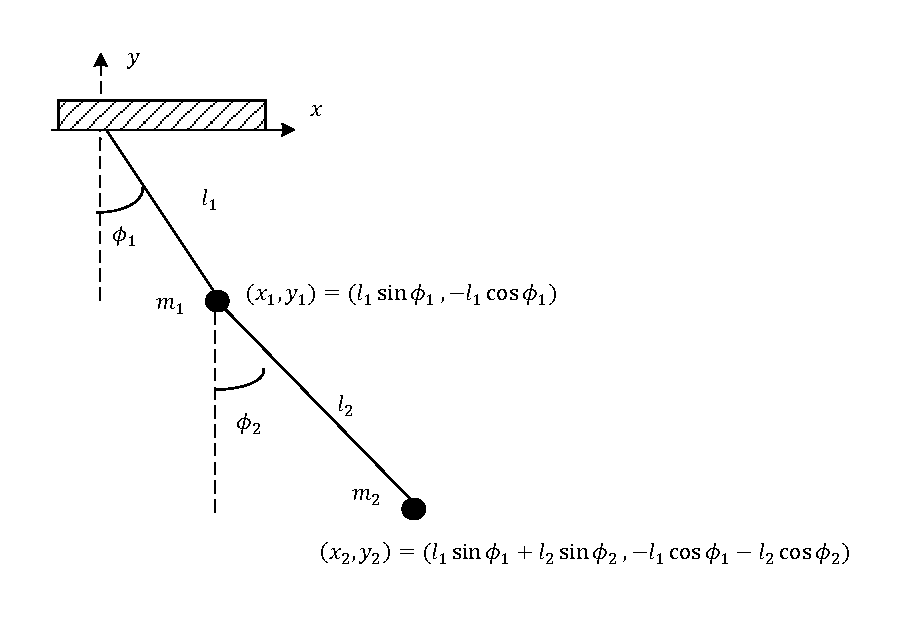
\includegraphics [width=10cm, height=8cm] {DoublePendulum}}
\caption{Pendulu bikoitza.}
\label{fig:41}
\end{figure} 

\subsubsection{Ekuazioak.}

\paragraph*{Hamiltondarra.}

\begin{equation*}
q=(\Theta_1,\Theta_2) \ \ , \ \ p=(P_1,P_2) \ \ , 
\end{equation*}

\begin{equation*} \label{eq:2}
H(q,p)= \bigg(\frac {C1 \ P_1^2 + C2 \ P_2^2 + 
 C3 \ P_1 \ P_2 \ \cos(\Theta_1 - \Theta_2)} {
 (C4 + C5 \ \sin^2 (Q_1 - Q_2))}\bigg)\\
       -C6 \ \cos(\Theta_1)-\ C7 \ \cos(\Theta_2), 
\end{equation*}

\paragraph*{}
     $C1 = l_2^2*m_2$,\\
     $C2 = l_1^2*(m_1 + m_2)$,\\
     $C3 = -2*l_1*l_2*l_2$,\\
     $C4 = 2*l_1^2*l_2^2*m_2*m_1$,\\
     $C5 = 2*m_1^2*l_2^2*m_2^2$,\\
     $C6 = g*l_1*(m_1 + m_2)$,\\
     $C7 = g*l_2*m_2$.


\paragraph*{Ekuazio diferentzialak.}

\begin{equation*}
\dot{\Theta_1}= \frac {2*C1*P1+C3*\cos(Q1-Q2)*P2}{aux1},
\end{equation*}

\begin{equation*}
 \ \ \dot{\Theta_2}= \frac{(2*C2*P2+C3*\cos(Q1-Q2)*P1)}{aux1},
\end{equation*}

\begin{equation*}
\dot{P1}=-(aux4+C6*\sin(Q1)), 
\end{equation*}

\begin{equation*}
\dot{P1}=(aux4-C7*\sin(Q2)), 
\end{equation*}

\paragraph*{}
$aux1=C4+C5*\sin(Q1-Q2)*\sin(Q1-Q2)$, \\
$aux2=C3*\cos(Q1-Q2)$,\\
$aux3=2*C5*\sin(Q1-Q2)*\cos(Q1-Q2)$,\\
$aux4=\frac{(-1/aux1^2)*(C1*P1^2+C2*P2^2+P1*P2*aux2)*aux3)-(C3*P1*P2*\sin(Q1-Q2))}{aux1}.$ 

\paragraph*{Jakobiarra.}
???

\subsubsection{Hasierako balioak.}

\paragraph*{\textbf{Sistemaren parametroak}.} 
Gure esperimentuetarako honako parametroak kontsideratuko ditugu,
\begin{equation*} \label{eq:17}
g=9.8 \ \frac{m}{sec^2}\,\ \ l_1=1.0 \ m \ , \ l_2=1.0 \ m\ , \ m_1=1.0 \ kg\ , \ m_2=1.0 \ kg
\end{equation*} 

\paragraph*{\textbf{Hasierako balioak}.}
Pendulu bikoitza konportamendu kaotikoa duen sistema ezlineala da. Zentzu honetan bi hasierako balio ezberdin kontsideratu ditugu \cite{Dumitru}:

\begin{enumerate}
   \item Hasierako balio ez-kaotikoak:   
   $q(0)=(1.1, 0)$ \ , \ $p(0)=(0,2.7746)$.
    
   \item Hasierako balio kaotikoak: \ \ \ \ \ \   
   $q(0)=(0,0)$ \ , \ \ \ \ $p(0)=(0,3.873)$.
\end{enumerate}


\subsubsection{Kodeak.}

Mathematican DoublePendulum.m paketean honako funtzioak inplementatu ditugu:

\begin{enumerate}
   \item Hamiltondarra: DoublePendulumHam.
   \item EDA: DoublePendulumODE.
   \item Jakobiarra: DoublePendulumJAC.
\end{enumerate}

\paragraph*{}C-lengoaian GaussUserProblem.c fitxategian honako funtzioak inplementatu ditugu:

\begin{enumerate}
   \item Hamiltondarra: HamPendulum().
   \item EDA: OdePendulum().
   \item Jakobiarra: JacPendulum().
\end{enumerate}

\subsection{N-Body problema.}

N gorputzeko problema grabitazionalari dagokionez, Eguzki sistemaren eredu sinplea integratuko dugu. Eguzki sistemaren gorputzak masa puntualak kontsideratuko ditugu eta gure ekuazio diferentzialek, gorputz hauen arteko erakarpen grabitazionalak bakarrik kontutan hartzen dituzte.Beraz, eguzki sistemaren eredu konplexuagoetako erlatibitate efektua, gorputzen formaren eragina, eta beste zenbait indar ez-grabitazionalak ez dira kontutan hartu.

$(N+1)$ gorputz kopurua izanik, $q_i,p_i\in \mathbb{R}^3, m_i \in \mathbb{R}$ gorputz bakoitzaren kokapena, momentua eta masa dira. Bestalde , momentua era honetan definituko dugu $p_i=m_i*v_i$ non $\frac{d q_i}{dt}=v_i$ den.


\subsubsection*{Equations.}

\paragraph*{Hamiltondarra.}

\begin{equation}
H(q,p)=\frac{1}{2}\ \sum^N_{i=0}{\ \frac{{\|p_i\|}^2}{m_i}}-G\ \sum^N_{0\le i<j\le N}{\frac{m_im_j}{\|q_i-q_j\|}} 
\end{equation}


\paragraph*{Ekuazio diferentzialak.}

\begin{equation}
\dot{q_i}=v_i, \  i=0,1,\dots N
\end{equation}

\begin{equation}
\dot{v_i}= \sum_{j=0,j \neq i}^{N} \frac{Gm_j}{\|q_j-q_i\|^3} (q_j-q_i)
\end{equation}

\paragraph{Jakobiarra.}

\begin{equation*}
\dot{y}=f(y)
\end{equation*}

\begin{equation}
Jac=\left(\begin{array}{cccccccc}
    \frac{\partial f_1}{\partial q_1} & \frac{\partial f_1}{\partial q_2} & \dots & \frac{\partial f_1}{\partial q_n} &
    \frac{\partial f_1}{\partial v_1} & \frac{\partial f_1}{\partial v_2} & \dots & \frac{\partial f_1}{\partial v_n}\\
    
    \dots & \dots & \dots & \dots & \dots & \dots & \dots & \dots \\
    
    \frac{\partial f_n}{\partial q_1} & \frac{\partial f_n}{\partial q_2} & \dots & \frac{\partial f_n}{\partial q_n} &
    \frac{\partial f_n}{\partial v_1} & \frac{\partial f_n}{\partial v_2} & \dots & \frac{\partial f_n}{\partial v_n}\\
  \end{array}\right)
\end{equation}

\paragraph*{}
And 2-body example,

\begin{equation}
J=\left(\begin{array}{cc}
  \ 0 & \ I \\
    A & \ 0 \\
\end{array}\right), \ \
Jac=\left(\begin{array}{ccccccccccccccc}
   & & q_{1x}  & q_{1y} & q_{1z}  & q_{2x}  & q_{2y} & q_{2z} & v_{1x}  & v_{1y} & v_{1z}  & v_{2x} & v_{2y} & v_{2z}  \\
   \\
   \frac{\partial f_1}{\partial q_{1x}} & & 0 & 0   & 0  & 0  & 0   & 0 & 1  &  0  & 0 & 0 & 0   & 0 \\
   \frac{\partial f_1}{\partial q_{1y}} & & 0 & 0   & 0  & 0  & 0   & 0 & 0  &  1  & 0 & 0 & 0   & 0 \\
   \frac{\partial f_1}{\partial q_{1z}} & & 0 & 0   & 0  & 0  & 0   & 0 & 0  &  0  & 1 & 0 & 0   & 0 \\
   \frac{\partial f_1}{\partial q_{2x}} & & 0 & 0   & 0  & 0  & 0   & 0 & 0  &  0  & 0 & 1 & 0   & 0 \\
   \frac{\partial f_1}{\partial q_{2y}} & & 0 & 0   & 0  & 0  & 0   & 0 & 0  &  0  & 0 & 0 & 1   & 0 \\
   \frac{\partial f_1}{\partial q_{2z}} & & 0 & 0   & 0  & 0  & 0   & 0 & 0  &  0  & 0 & 0 & 0   & 1 \\
   
   \frac{\partial f_1}{\partial v_{1x}} & & A & A   & A  & A  & A   & A & 0  &  0  & 0 & 0 & 0   & 0 \\
   \frac{\partial f_1}{\partial v_{1y}} & & A & A   & A  & A  & A   & A & 0  &  0  & 0 & 0 & 0   & 0 \\
   \frac{\partial f_1}{\partial v_{1z}} & & A & A   & A  & A  & A   & A & 0  &  0  & 0 & 0 & 0   & 0 \\
   \frac{\partial f_1}{\partial v_{2x}} & & A & A   & A  & A  & A   & A & 0  &  0  & 0 & 0 & 0   & 0 \\
   \frac{\partial f_1}{\partial v_{2y}} & & A & A   & A  & A  & A   & A & 0  &  0  & 0 & 0 & 0   & 0 \\
   \frac{\partial f_1}{\partial v_{2z}} & & A & A   & A  & A  & A   & A & 0  &  0  & 0 & 0 & 0   & 0 \\
  \end{array}\right)  
\end{equation}

\paragraph*{}Eta $A$ matrizearen deskribapena honako notazioaren laguntzaz,
\begin{equation*}
q_j-q_i=(x_{ji},y_{ji},z_{ji})
\end{equation*}
\begin{equation*}
\sum = \sum_{j=0,j \neq i}^{N}
\end{equation*}


\begin{enumerate}
\item $i==j$.\\
\begin{equation*}
A=\left(\begin{array}{ccc}
  \ \sum \bigg(\frac{3*Gm_j*x_{ji}^2}{\|q_j-q_i\|^5}\bigg)-
    \sum \bigg(\frac{Gm_j}{\|q_j-q_i\|^3} \bigg)& 
  \ \sum \bigg(\frac{3*Gm_j*(x_{ji}*y_{ji})}{\|q_j-q_i\|^5}\bigg)& 
  \ \sum \bigg(\frac{3*Gm_j*(x_{ij}*z_{ji})}{\|q_j-q_i\|^5}\bigg) \\
  
  \ \sum \bigg(\frac{3*Gm_j*(y_{ji}*x_{ji})}{\|q_j-q_i\|^5}\bigg)& 
  \ \sum \bigg(\frac{3*Gm_j*y_{ji}^2}{\|q_j-q_i\|^5}\bigg)-
          \sum \bigg(\frac{Gm_j}{\|q_j-q_i\|^3} \bigg)& 
    \ \sum \bigg(\frac{3*Gm_j*(y_{ji}*z_{ji})}{\|q_j-q_i\|^5}\bigg) \\
  
   \ \sum \bigg(\frac{3*Gm_j*(z_{ji}*x_{ji})}{\|q_j-q_i\|^5}\bigg)& 
   \ \sum \bigg(\frac{3*Gm_j*(z_{ji}*y_{ji})}{\|q_j-q_i\|^5}\bigg)& 
   \ \sum \bigg(\frac{3*Gm_j*z_{ji}^2}{\|q_j-q_i\|^5}\bigg)-
     \sum \bigg(\frac{Gm_j}{\|q_j-q_i\|^3} \bigg) \\
  
\end{array}\right)
\end{equation*}

\item $i \neq j$. \\
\begin{equation*}
A=\left(\begin{array}{ccc}
  \ \bigg(\frac{-3*Gm_j*x_{ji}^2}{\|q_j-q_i\|^5}\bigg)+
    \bigg(\frac{Gm_j}{\|q_j-q_i\|^3} \bigg)& 
  \ \bigg(\frac{-3*Gm_j*(x_{ji}*y_{ji})}{\|q_j-q_i\|^5}\bigg)& 
  \ \bigg(\frac{-3*Gm_j*(x_{ij}*z_{ji})}{\|q_j-q_i\|^5}\bigg) \\

  \ \bigg(\frac{-3*Gm_j*(y_{ji}*x_{ji})}{\|q_j-q_i\|^5}\bigg)& 
  \ \bigg(\frac{-3*Gm_j*y_{ji}^2}{\|q_j-q_i\|^5}\bigg)+
    \bigg(\frac{Gm_j}{\|q_j-q_i\|^3} \bigg)& 
  \ \bigg(\frac{-3*Gm_j*(y_{ji}*z_{ji})}{\|q_j-q_i\|^5}\bigg) \\
  
   \ \bigg(\frac{-3*Gm_j*(z_{ji}*x_{ji})}{\|q_j-q_i\|^5}\bigg)& 
   \ \bigg(\frac{-3*Gm_j*(z_{ji}*y_{ji})}{\|q_j-q_i\|^5}\bigg)& 
   \ \bigg(\frac{-3*Gm_j*z_{ji}^2}{\|q_j-q_i\|^5}\bigg)+
     \bigg(\frac{Gm_j}{\|q_j-q_i\|^3} \bigg) \\  
  
\end{array}\right)
\end{equation*}

\end{enumerate}

\subsubsection*{Hasierako balioak.}

The initial conditions and parameters have been taken from JPL Solar System ephemerids DE-405.
We have modified the velocities to get zero linear momentum.

\subsection{Inplementazioak.}

\paragraph*{} Mathematicako NBodyProblem.m paketean honako funtzioak garatu ditugu.

\begin{enumerate}
   \item Hamiltondarra: NBodyHAM.
   \item EDA: NBodyODE.
   \item Jakobiarra: Ez dut garatu.
\end{enumerate}

-\paragraph*{} C-lengoaiako inplementazioa:

\begin{enumerate}
   \item Hamiltondarra: HamNBody().
   \item EDA: OdeNbody().
   \item Jakobiarra: JacNBody().
\end{enumerate}




\section{Koma Higikorreko Aritmetika.}

\subsection{Sarrera.}

Gaur-egungo konputagailuetan,  IEEE-754 estandarraren araberako koma-higikorreko artimetika erabiltzen da. Koma-higikorreko aritmetikaren gaiak ez dira zenbaki errealak, koma-higikorreko zenbakiak baizik. Zenbaki errealak bit kopuru finituen bidez adierazten dira eta adierazpen finitu honek, biribiltze errorea eragiten du. Zenbakizko integrazio luzeetan  biribiltze errorearen garapenak garrantzia handia du eta errore honen gaineko ahalegin berezia beharrezkoa da.    

\subsection{Adierazpena.}

\paragraph*{\textbf{Definizioa}.}  Koma-higikorreko adierazpen zehatza duen zenbaki errealei koma-higikorreko zenbakiak deritzogu. Koma-higikorreko zenbakien multzoa ${\mathbb{F}}$ izendatuko dugu eta $\phi:\mathbb{F} \rightarrow W$ koma-higikorreko adierazpen funtzioa. 

\begin{equation*}
\mathbb{F}\subset \mathbb{R},
\end{equation*}
\begin{equation}
\mathbb{F}=\{x \in \mathbb{R} \ \mid \ \phi(x) \in W\}.
\end{equation}

\paragraph*{}$\mathbb{F}$ zenbaki multzoa finitua da. Bai zenbaki positiboentzat,bai negatiboentzat, adieraz daitekeen zenbaki handienaren eta txikienaren arteko balio bakanez osatuta dago. Multzoaren kanpokaldean zenbaki hauek guztiak ditugu: batetik overflow tartean $(-\infty,\max_{x \in \mathbb{F_{-}}}|x|)$  eta $(\max_{x \in \mathbb{F_{+}}}|x|,\infty+)$ daudenak; bestetik underflow tartean  $(\min_{x \in \mathbb{F_{-}}}|x|,0)$ eta $(0,\min_{x \in \mathbb{F_{+}}}|x|)$ daudenak. 

\begin{figure}[h]
\centerline{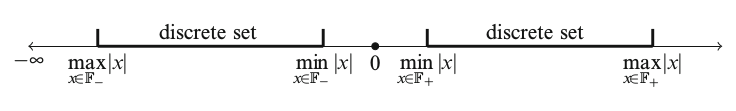
\includegraphics[width=12cm, height=2cm] {KomaHigikorra1}}
\caption{Floating-point number line.}
\label{fig:three}
\end{figure} 

\paragraph*{} IEEE-785 estadarraren arabera, $n$-biteko koma-higikorrezko adierazpenak bi zati ditu,
\begin{enumerate}
\item $m$ bitez osatutako zatia , mantisa deitutakoa eta $M$ zenbaki erreala adierazten duena. Horietako bit bat ($S_M$) zeinua adierazten du. Bestalde $M$ mantisa modu normalizatu honetan emana da, $\pm 1.F$ eta zati erreala ($F$) bakarrik gordetzen da.   
\item Exponentea ($E$), $(n-m)$ bitez adierazitako zenbaki osoa. Zeinuarentzat ez da bit zehatz bat erabiltzen, baizik \it {bias} izeneko balio bat gehituz adierazten dira zenbaki positiboak eta negatiboak.  
\end{enumerate}

\paragraph*{} Eta beraz, oinarri bitarrean koma-higikorreko zenbaki hauek adierazten dira,
\begin{equation*}
M \times b^E, \ b=2.
\end{equation*}

\begin{figure}[h]
\centerline{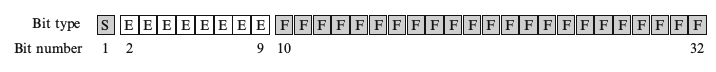
\includegraphics[width=10cm, height=1cm] {KomaHigikorra2}}
\caption{\small 32-biteko koma-higikorreko zenbakiaren adierazpena: exponentearentzat 8 bit eta mantisarentzat 24 bit (bit bat zeinuarentzat eta beste 23 bit, $1.F$ eran normalizatutako mantisarentzat) banatuta.}
\label{fig:three}
\end{figure} 

\paragraph*{} 
Bi koma-higikor zenbaki jarraien arteko diferentzia,
\begin{equation*}
\triangle x=x_1-x_2= 2^{E-m+1}
\end{equation*} 

\paragraph*{}
\it {Machine epsilon} ($\epsilon_M$), $E=0$ deneko koma-higikorrezko bi zenbakien arteko diferentzia bezala definitzen da,
\begin{equation*}
\epsilon_M=2^{-m+1}
\end{equation*} 

\paragraph*{}
Azkenik, \it{roundoff} definituko dugu zenbaki erreal batek koma-higikorrean adierazpenean izan dezakeen errore erlatibo maximoa bezala,
\begin{equation*}
u=\frac{\epsilon_M}{2}=2^{-m}
\end{equation*}  


\paragraph*{}IEEE-785 estandarrean honako formatu bitarrak definitzen dira:

\begin{table} [h!]
\caption{}
\label{tab:1}       % Give a unique label
\begin{tabular}{ |c|c|c|c|c|c|} 
\hline
 Mota      &  Tamaina    & m   & e  & Tartea           &  $u=2^{-m}$           \\ \hline
           &             &     &    &                  &                       \\
% Half      & 16 bit      & 11  & 5  & $2^{\pm 16}$     &  $5 \times 10^{-4}$   \\ 
 Single    & 32 bit      & 24  & 8  & $10^{\pm 38}$    &  $6 \times 10^{-8}$   \\	    
 Double    & 64 bit      & 53  & 11 & $10^{\pm 308}$   &  $1 \times 10^{-16}$   \\
 Quadruple & 128 bit     & 113 & 15 & $10^{\pm 11356}$ &  $1 \times 10^{-35}$   \\
\hline
\end{tabular}
\end{table}

Gaur egungo konputagailuetan, Single eta Double koma-higikorreko aritmetika Hardwarez inplementatuta dago eta oso azkarrak dira. Single koma-higikorreko aritmetikak Double baino azkarragoa da: batetik garraiatu behar den bit kopuru erdia da eta bestetik, Inteleko txipen \it SSE modulo bereziei esker eragiketa artihmetikoak azkarragoak dira.

2008. urtean, IEEE-785 estandarrak 128 biteko koma-higikorreko aritmetika onartu zuen. Quadruple aritmetika softwarez inplementatuta dago eta horregaitik exekuzio motela da, gutxigorabehera Double aritmetika bainon 10 aldiz garestiago. Horretarako hainbat liburutegi daude, guk GCC libquadmath liburutegia aukeratu dugu gure garapeneterako.

Bestalde, badaude doitasun arbitrariotan lan egiteko beste software batzuk ere. Doitasun altuetako kalkulu hauekin, soluzio zehatzak lortzen dira eta horrela, algoritmoen testak egiteko bidea ematen dute. Matlab eta Mathematica bezalako softwareetan doitasun handian lan egiteko aukera ematen dute eta beraz, algoritmo berri baten garapenean oso tresna erabilgarriak izan daitezke.

 
\subsection{Biribiltze errorea.}

Bi motako biribiltze errorea dugu, bata adierzapen errorea eta beste eragiketa (aritmetika) errorea.  

\subsubsection*{Adierazpen errorea.} 

$x \in \mathbb{R}$ eta $fl: \mathbb{R} \rightarrow \mathbb{F}$ 
koma-higikorreko zenbaki gertuen esleitzen duen funtzioa emanik, errore absolutuaren  $\triangle x$ definizioa,

\begin{equation*}
\triangle x= fl(x)-x= \tilde{x}-x,  
\end{equation*}    
 
eta errore erlatiboa, 
\begin{equation*}
\delta x =\frac{\triangle x}{x} = \frac{\tilde{x}-x}{x}. 
\end{equation*}

Aurreko bi definizioen ondorioz honako formula erabilgarria dugu,
\begin{equation*}
\tilde{x}= x+\triangle x = x(1+\delta x),
\end{equation*}
zeinek IEEE-785 estandarrak $|\delta x|<u$ dela bermatzen duen.

\subsubsection*{Eragiketen errorea.} 
 
Zenbaki errealen arteko funtsezko eragiketak  $\ast: \mathbb{R}^2\rightarrow \mathbb{R}$, hauek dira
\begin{equation*}
\ast\in \{+,-,x,/ \}.
\end{equation*}

Modu berean, koma-higikorrezko zenbakien arteko funtsezko eragiketak hauek dira $\circledast: \mathbb{F}^2\rightarrow \mathbb{F}$
\begin{equation*}
\circledast\in \{\oplus,\ominus,\otimes,\oslash \}.
\end{equation*}

$\tilde x,\tilde y \in \mathbb{F}$ emanik eta $z= \tilde x \ast \tilde y$ emaitza zehatza bada, $\tilde z= \tilde x \circledast \tilde y$ eragiketaren emaitzaren errore absulotua eta erlaziboak definituko ditugu,
\begin{equation*}
\triangle z=\tilde z-z =(\tilde x \circledast \tilde y) -(\tilde x \ast \tilde y)
\end{equation*} 

\begin{equation*}
\delta z=\frac{\triangle z}{z}==\frac{(\tilde x \circledast \tilde y) -(\tilde x \ast \tilde y)}{(\tilde x \ast \tilde y)}
\end{equation*} 

\begin{equation*}
\tilde z=(\tilde x \circledast \tilde y)=z+\triangle z=z(1+\delta z), \ |\delta z|<u. 
\end{equation*}


\paragraph*{\textbf{Adibidea.}}
Errore erlatiboak emitzaren digitu zuzenak neurtzen du:
\begin{equation*}
\delta z \approx 10^{-k} \Rightarrow \ \approx \ k \ digitu \ zuzen.
\end{equation*}  

\subsubsection*{Ezabapen arazoa.}

Algoritmoen kalkuluetan, doitasuna galera azkarra gerta daiteke. Horren adibidea ezabapen arazoa dugu: oso antzekoak diren bi zenbaki kentzen ditugunean gerta daitekeena. 

\paragraph*{\textbf{Adibidea}}.

CatastrophicCancelation.nb adibidea idatzi.


\begin{lstlisting}
>>  InputForm[N[Pi]]
>> 3.141592653589793

>> y=N[Pi]*10^(-10);
>> InputForm[y]
>> 3.1415926535897934*10^(-10)

>> z=1.+y;
>> InputForm[z]
>> 1.0000000003141594

>> InputForm[z-1.]
>> 3.141593651889707*10^(-10)

\end{lstlisting}
 

\subsubsection*{Errore propagazioa.}

Konputazioetan eragiketa aritmetiko kopuru handia egin behar dugu emaitza lortzeko eta biribiltze errorea metatu daiteke. Batzuetan, eragiketa bakoitzeko biribiltze errorea elkar ezereztatzen da baina kasu txarrenean, biribiltze errorea metatu eta magnitude handikoa izan daiteke.   

\paragraph*{\textbf{Adibidea}.} 
Modu honetako batura batean , non $n>2$ eta $\tilde x_1,\dots,\tilde x_n \in \mathbb{F}$,  ezin daiteke bermatu,  
\begin{equation*}
\bigoplus_{i=1}^{n}(\tilde x_i)=(\sum\limits_{i=1}^{n} \tilde x_i)(1+\delta), \ |\delta|<u.
\end{equation*}

\paragraph*{}Eta $n=3$ deneko adibidean,
\begin{equation*}
((\tilde x_1 \oplus \tilde x_2) \oplus \tilde x_3)  = 
  (\tilde x_1 + \tilde x_2)(1+\delta_1)(1+\delta_2)
  +\tilde x_3 (1+\delta_2), \ \ \delta_1,\delta_2<u.
\end{equation*}

\subsubsection{Tresnak.}
\subsubsection*{Batura konpensatua.}
   
Batura errekurtsiboetan, biribiltze errorea gutxitzeko metodoa dugu.
Ideia da, bi zenbakien baturan egindako biribiltze errorearen estimazioa lortu eta estimazio hau hurrengo baturan erabiltzea.

\paragraph*{} Estimazioa nola kalkulatu azaltzeko ikus irudia (Fig. \ref{fig:lau}). Koma-higikorreko bi zenbaki baditugu, $\tilde x,\tilde y \in \mathbb{F}$ non $|\tilde x| \geq |\tilde y|$, eta $\tilde z= \tilde x \oplus \tilde y$ ,

\begin{equation*}
\tilde e= - \bigg(\big(( \tilde x \oplus \tilde y) \ominus \tilde x\big) \ominus \tilde y\bigg) = (\tilde x \ominus \tilde z) \oplus \tilde y
\end{equation*}  

\begin{figure}[h]
\centerline{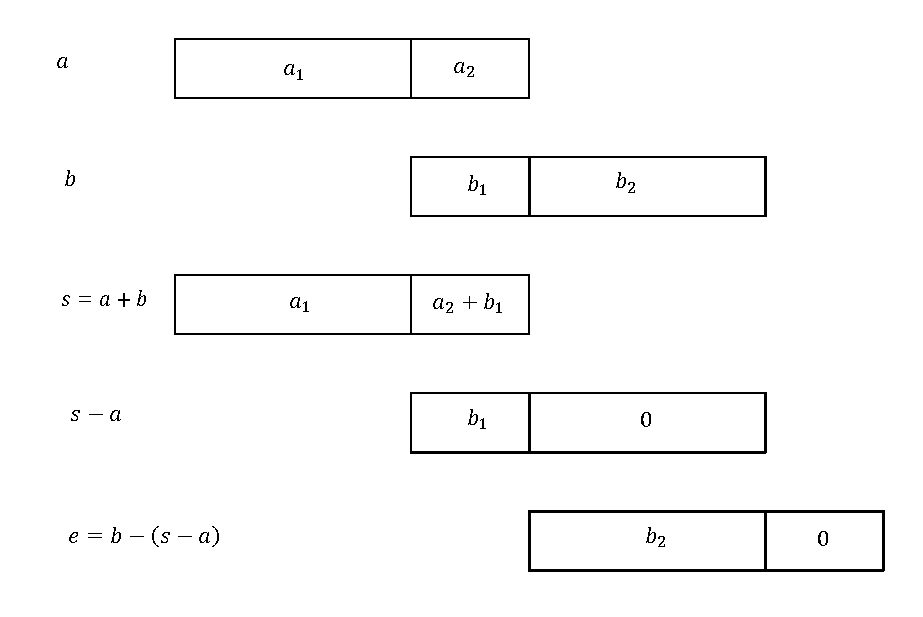
\includegraphics[width=12cm, height=4cm] {Quick2Sum}}
\caption{Biribiltze errorea.}
\label{fig:lau}
\end{figure} 

Lortutako errore estimazioa, koma-higikorreko aritmetikan zehazki benetazko biribiltze errorea da (frogapena Kahan),
\begin{equation*}
\tilde x+\tilde y= \tilde z+\tilde e.
\end{equation*}

\paragraph*{} Batura konpensatu algoritmoa biribiltze errore honen estimazioan oinarritzen da. Honako batura  $z=\sum\limits_{i=1}^{n} \tilde x_i$ kalkulatzeko , urrats bakoitzaren amaieran errore estimazioa ($e$) kalkulatuko dugu eta hurrengo urratsean,  batugaiari gehituko diogu ($y=\tilde x_i+e$).

\begin{algorithm}[H]
 \BlankLine
  $z=0; e=0$\;
  \For{$i\leftarrow 1$ \KwTo $endstep$}
  {
   \BlankLine
    $x=z$\;
    $y=\tilde x_i+e$\;
    $z=x+y$\;
    $e=(x-z)+y$\;
   \BlankLine
  }
 \caption{Batura konpensatua.}
\end{algorithm}

\subsection*{Theorem Sterbenz}.
Let x and y be floating point numbers with $\frac{y}{2}\leq x \leq 2y$. Then $x-y$ is computed exactly (assuming $x-y$ does not underflow.

\subsection*{FMA.}
IEEE-785 (2008 revision).

\begin{equation*}
\tilde x \otimes \tilde y \oplus \tilde z= (\tilde x \times \tilde y+ \tilde z) (1+\delta), \ \delta<u 
\end{equation*}

\subsection{Laburpena.}




\section{Scientific Computing.}

\subsection{Sarrera.}

Gaur-egun, orohar konputagailuak (superkonputagailu, portatila,...) paraleloak dira. 1986-2002 urteen artean,  prozesadore bakarreko konputagailuen eraginkortasuna hobetuz joan zen, txipean transistore dentsitatea handitzen zen heinean   baina teknologi-garapena muga fisikoetara iritsita, bide honetatik konputagailuen abiadura hobetzea ezinezkoa bilakatu zen. Horrela, 2005.urtetik aurrera fabrikatzaileek konputagailuen gaitasuna hobetzeko, txipan prozesadore bat baino gehiago erabiltzea erabaki zuten.      

\paragraph*{Moore's Law (1965)}. Processor speed doubles every 18 months.

\paragraph*{Moore's Law Reinterpreter}. Number of cores per chip can double every two years.

\begin{figure}[h]
\centerline{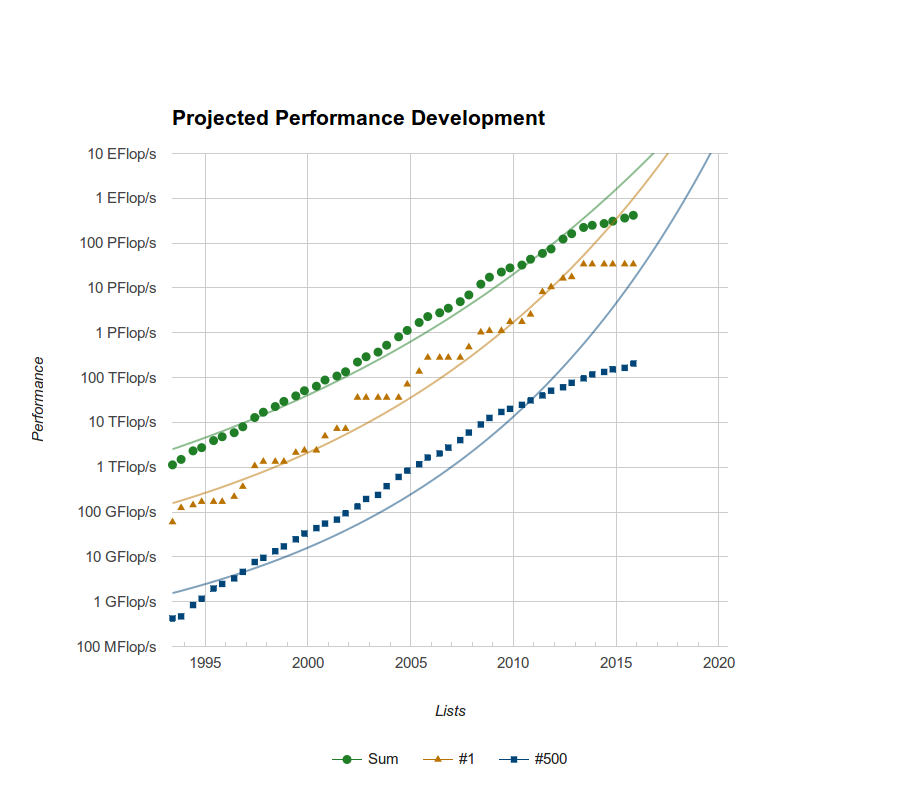
\includegraphics[width=12cm, height=8cm] {PerformanceDevelopment}}
\caption{www.top500.org, Top: total computing power of top 500 computers. Middle: 1 computer. Bottom: 500 computer.}
\label{fig:61}
\end{figure} 

\paragraph*{} Konputagailuen eredu aldaketa honen ondorioz, algoritmo azkarrak garatzeko kodearen paralelizazio gaitasunari heldu behar zaio. Beraz programazio paralelo teknikak inplementatzeko, beharrezko da prozesadore berrien hardware arkitekturak nahiz software ingurune berriak ulertzea. Gaia nahiko konplexua izanik, ikuspegi orokorra eman ondoren, gure inplementazioan erabilitako hardware arkitektura eta software teknika zehatzak azalduko ditugu. Memoria-konpartitutako sistemak eta OpenMP programazio eredua deskribatuko dugu.

\paragraph*{}Bi dira, algoritmo azkarrak disenatzeko erronkak: 
\begin{enumerate}
\item Paralelizatzeko pisuko lana identifikatzea.
\item Memoria eta prozesadorearen arteko datu mugimendua gutxitzea. 
\end{enumerate}

\paragraph*{}Bestalde, inplementazio berrien garapenean optimizatutako liburutegiak erabiltzea komeni da. Horien artean, LAPACK eta BLAS algebra linealeko liburutegiak erabilgarriak izan zaizkigu. Liburutegi hauen gaineko azalpenak emango ditugu.

\subsection{Parallel Hardware.}

\subsubsection*{\textbf{Zein azkarrak dira konputagailuak?}}

\paragraph*{}Gaur egungo prozesadoreen abiadura Gigahertzioetan neurtzen da. 

\begin{itemize}
\item Kilo = mila ($10^3$).
\item Mega = milioi ($10^6$).
\item Giga = bilioi ($10^9$).
\item Tera = trilioi ($10^{12}$).
\item Peta = $10^{15}$.
\item Exa = $10^{18}$. 
\end{itemize}

\paragraph*{} Hertzioak "makina zikloak segunduko" esan nahi du. Koma-higikorrezko  eragiketa bat egiteko ($\oplus,\ominus,\otimes,\oslash$) ziklo gutxi batzuk behar dira. Honek esan nahi du, $1$GHz-ko prozesagailu batek,
$>100.000.000$ koma-higikorrezko eragiketa segunduko egiten dituela ($>100$ Megaflops).

\paragraph*{\textbf{Adibidea}}. 
$C=AB$ matrize-matrize biderketa.

\paragraph*{}Demagun $A,B$ eta $C \ (n \times n)$ dimentsioko matrizeak.

\begin{equation*}
c_{ij}=\sum\limits_{i,j=1}^{n} a_{ij}*b_{ji}
\end{equation*}

\paragraph*{} $c_{ij}$ gai bakoitza kalkulatzeko $n$ biderketa eta ($n-1$) batura egin behar ditugu.

$C$ matrizeak $n^2$ osagaia ditu $\Rightarrow$ $O(n^3)$ koma-higikorrezko ariketak.

$n=1000 \ \Rightarrow \ n^3=10^{12}$

$>1000$ segundu $1$GHz prozesagailuan.

\paragraph*{} Zientzia konputazioaren eraginkortasuna neurtzeko, koma-higikorrezko eragiketa kopurua (flops) erabiltzen zen. Problema handia denean, datuen mugimendua koma-higikorrezko eragiketak baino garestiagoa da, eta beraz eraginkortasuna aztertzeko koma-higikorrezko eragiketa kopurua neurtzea okerra izan daiteke. Kodearen exekuzioa azkartzeko derrigorrezkoa da konputagailuan datuen mugimendua minimizatzea.

\subsubsection*{\textbf{Memoria Hierarkia.}}

\paragraph*{}Lehenik, konputagailuan dauden memoria mota ezberdinen hierarkia azalduko dugu. 

\begin{figure}[h]
\centerline{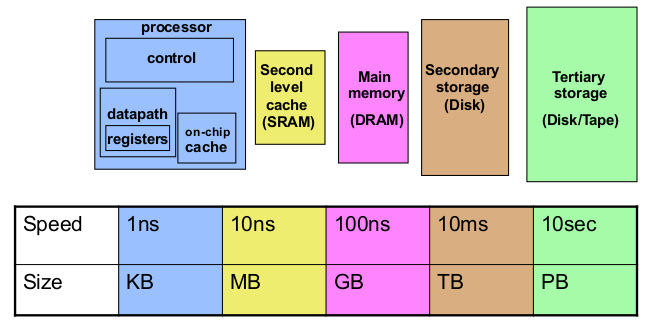
\includegraphics[width=10cm, height=4cm] {MemoryHierarchy}}
\caption{Memoria hierarkia.}
\label{fig:three}
\end{figure} 

\paragraph*{} CPU-k koma-higikorrezko eragiketak egiten ditu: datuak erregistroetatik irakurri, eragiketa egin eta emaitza erregistroetan idazten ditu. Memoria nagusia eta erregistroen artean, 2 edo 3 mailako Cache memoria dugu: lehen Cache memoria (L1) txikiena eta azkarrena da, eta beste mailak (L2,L3,...), handiagoak eta motelagoak. Memoria nagusian, exekutatzen diren programak eta datuak gordetzen dira ($1-4$ GB artekoa). Azkenik, disko gogorrean konputagailuko datu (argazki, bideo,...) eta erabilgarri ditugun programa guztiak gordetzen dira.  
   
\paragraph*{} Cache memorian, programak hurrengo unean behar dituen datuak gertu dauden printzipioaren arabera gordetzen da informazioa. Cache memoria blokeka (line) egituratuta dago eta bloke bakoitza $64$ edo $128$ bytez ($8$ edo $16$ double zenbaki) osatuta dago. 

\paragraph*{\textbf{Adibidea}}. Badakigunez, C-lengoaian matrizeak lerroka gordetzen dira. Beheko adibidean,  matrizearen lehen osagaia $a(1,1)$ behar dugunean, memoria nagusitik Cachera osagai honetaz gain jarraiko 16 osagaiak ekarriko dira ($a(1,1),a(1,2),\dots,a(1,16)$). Honela, hurrengo $15$ batura egiteko behar ditugun datuak Cachean eskuara izango ditugu memoria irakurketa berririk egin gabe. 

\begin{algorithm}[h]
 \BlankLine
  $int \ n$\;
  $double \ a[n][n]$\;
  \BlankLine
  $sum=0$\;
  \For{$i\leftarrow 1$ \KwTo $n$}
  {
   \BlankLine
    \For{$j\leftarrow 1$ \KwTo $m$}
   {
    \BlankLine 
    $sum+=a(i,j)$\;
   }
 }
 \caption{Main Algorithm}
\end{algorithm} 

\begin{equation*}
a=\left(\begin{array}{ccccc}
  1    & 2    & 3    & \dots & 1000 \\
  1001 & 1002 & 1003 &\dots & 2000 \\
  2001 & 2002 & 2003 &\dots & 2000 \\
  \dots & \dots & \dots & \dots & \dots \\
  9001 & 9002 & 9003 &\dots & 10000 \\
  \end{array}\right).  
\end{equation*}

\paragraph*{}CPUk datu bat behar duenean, memoria hierarkian zehar bilatuko du: lehenik $L1$ cachean, ondoren $L2$ cachean,...eta hauetan ez badago, memoria nagusira joko du. Memoria nagusi eta cache memoria arteko irakurketa eta idazketa guzti hauetan,  informazio konsistentzia mantentzeko hainbat arau aurrera ematen dira.  

\subsubsection*{\textbf{Hardware.}}

MIMD (Multiple instruction, multiple data) sistemak, guztiz independienteak diren prozesadore multzoak osatzen dituzte. Bi dira MIMD sistema nagusiak: memoria konpartitutako eta memoria distribuitutako sistemak. Memoria konpartitutako sistemetan, prozesadore guztiek memoria osoa konpartitzen dute eta inplizituki konpartitutako datuen atzipenaren bidez komunikatzen dira. Memoria distribuitutako sistemetan aldiz, prozesadore bakoitzak bere memoria pribatua du eta explizituki bidalitako mezuen bidez komunikatzen dira.

\paragraph*{} Hirugarren hardware arkitektura ere aipatuko dugu, general purpose GPU computing (Graphical Processor Unit).
Jokuen eta animazio industriak, grafiko oso azkarrak beharrak biltzatuta  sortutako teknologia da. Oinarrian, imaginak oantailaratzeko prozesagailu asko paraleloan lan egiten dute. Azken hamarkadan, GPU unitate hauek zientzia konputaziora zabaldu dira.  

\begin{figure}[h]
\centerline{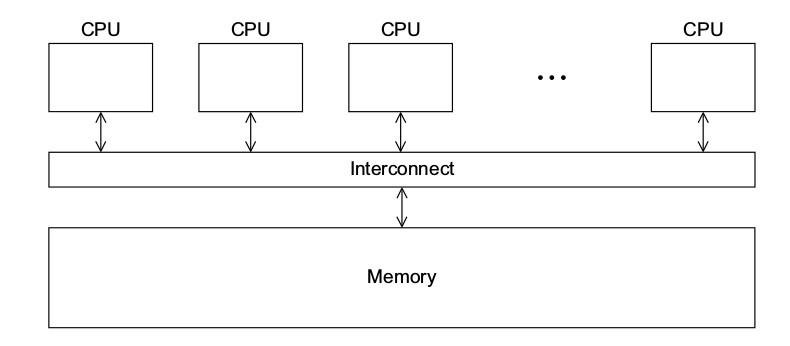
\includegraphics[width=12cm, height=4cm] {SharedMemorySystem}}
\caption{Shared Memory System.}
\label{fig:61}
\end{figure}  

\begin{figure}[h]
\centerline{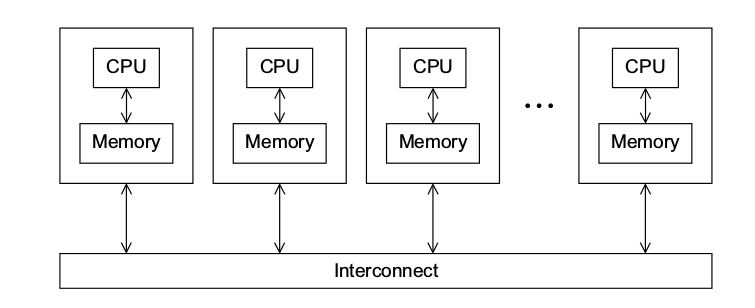
\includegraphics[width=12cm, height=4cm] {DistribuitedMemorySystem}}
\caption{Distribuited Memory System.}
\label{fig:61}
\end{figure}  

\paragraph*{\textbf{Shared-memory systems}}. Multicore bat edo gehiagoz osatutako sistema dugu. Multicore prozesadore bakoitzak txipean CPU bat baino gehiago ditu. Normalean CPU bakoitzak $L1$ bere cache memoria du. Aipatzeko da, era honetako sistemetan prozesadore kopurua ezin dela nahi adina handitu eta mugatua dela (normalean $\leq 32$ ).

 \begin{figure}[h]
 \centerline{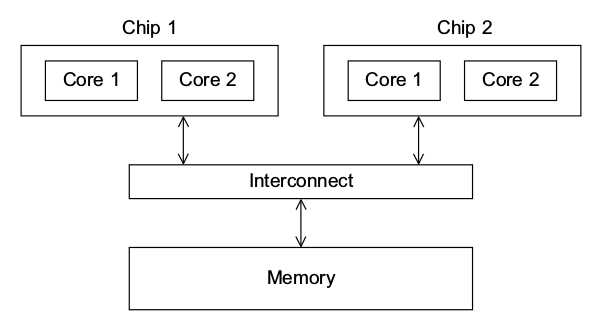
\includegraphics[width=12cm, height=4cm] {SharedMemorySystemUMA}}
 \caption{Shared Memory System (UMA).}
 \label{fig:61}
 \end{figure}  

\subsubsection*{\textbf{Sofwarea.}}

C-lengoaia programazio paraleloan erabiltzeko, lengoiaren bi extensio dira nagusienak: bata memori-distribuitutako sistemetarako diseinatuta  MPI (Message-Passing Inteface) eta bestea, memoria-konpartitutako sistemetarako diseinutakoa OpenMP (Open Specifications for MultiProcessing). MPI datu moten definizio, funtzio eta makroen liburegia da. OpenMP liburutegia bat  eta C konpiladorearen aldaketa batzuk. OpenMP erabili dugu gure inplementaziorako eta jarraian honi buruzko idei nagusienak emango ditugu.

\paragraph*{\textbf{OpenMP}}. Memoria konpartitutako programazio paraleloaren estandarra dugu. 
Programazioan paralelizazio kontrola, "fork-join" modeloa jarraituz egiten da.

\begin{enumerate}
\item OpenMP programen hasieran prozesu bakarra dago, hari (thread) nagusia. 
\item FORK: hari nagusiak hari talde paraleloa sortzen du.
\item JOIN: hariak kode paraleloa bukatzen dutenean, behin sinkronizatuta amaitzen dute eta hari nagusiak bakarrik jarraitzen du.
\end{enumerate}

 \begin{figure}[h]
 \centerline{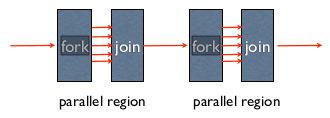
\includegraphics[width=10cm, height=3cm] {ForkJoin}}
 \caption{Fork-Join.}
 \label{fig:61}
 \end{figure}  

Aldagai batean (threadcount) paralelizazioan zenbat hari erabili adierazten da eta ohikoa izaten da hari bat prozesadore bakoitzeko sortzea.  Konpilazio direktiben bidez,  paralelizazioa nola exekutatu behar den zehazten zaio.

\paragraph*{\textbf{Adibidea}}.

\begin{lstlisting}
#    pragma omp parallel for num_threads(thread_count) 
     for (i = 0; i<n; i++)
     {
       ! Aginduak 
     }
\end{lstlisting}

\subsection{Software liburutegiak.}

Matematika bi software errekurtso nagusienak aipatuko ditugu; BLAS (Basic Linear Algebra Subroutines) eta LAPACK (Linear Algebra Package). Kalitate handiko software orokorrak dira eta hauek erabiltzea abantaila asko ditu: 

\begin{enumerate}
\item Garapen berriak egiteko denbora aurrezten du. 
\item Problema askotan ondo probatutako softwareak dira.
\item Konplexutasun handikoak dira, modu seguruan eta azkarrean exekutatzeko disenatu direlako. 
\end{enumerate}

Konputagailu hardware bakoitzerako optimizatutako bertsioak daude. Inplementazioa Fortranen egina dago eta datu-motei dagokionez:

\begin{enumerate}
\item S: float ($32$ bit).
\item D: double ($64$ bit).
\item C: complex.
\item Z: complex double.
\end{enumerate}   

\subsubsection*{\textbf{BLAS}}.

BLAS liburutegian, bektore eta matrizeen arteko funtzio estandarrak inplementatuta daude. Hiru mailetan banatuta dago: 

\begin{enumerate}
\item BLAS-1: bektore-bektore eragiketak.

 Adibidez: $y=\alpha*x+y$ , $2n$ flop eta $3n$ irakurketa/idazketa.
 
 Konputazio intentsitatea: $\frac{2n}{3n}=\frac{2}{3}$. 

\item BLAS-2: matrize-bektore eragiketak.

 Adibidez: $y=\alpha*A*x+\beta*x$, $O(n^2)$ flop eta $O(n^2)$ irakurketa/idazketa.
 
 Konputazio intentsitatea: $\approx \frac{2n^2}{n^2}=2$. 
 
\item BLAS-3: matrize-matrize eragiketak.

 Adibidez: $C=\alpha*A*B+\beta*C$, $O(n^3)$ flop eta $O(n^2)$ irakurketa/idazketa.
 
 Konputazio intentsitatea: $\approx \frac{2n^3}{4n^2}=\frac{n}{2}$. 

\end{enumerate}

Azpimarratu, BLAS-1 eta BLAS-2 funtzioen konputazio intetsitatea txikia dela eta beraz, datuen komunikazioa nagusia dela. BLAS-3 aldiz, konputazio intentsitatea handiagoa da eta eazugarri honi esker, konputagailuaren konputazio gaitasuna ondo aprobetxatu ahal izango da.

\begin{figure}[h]
\centerline{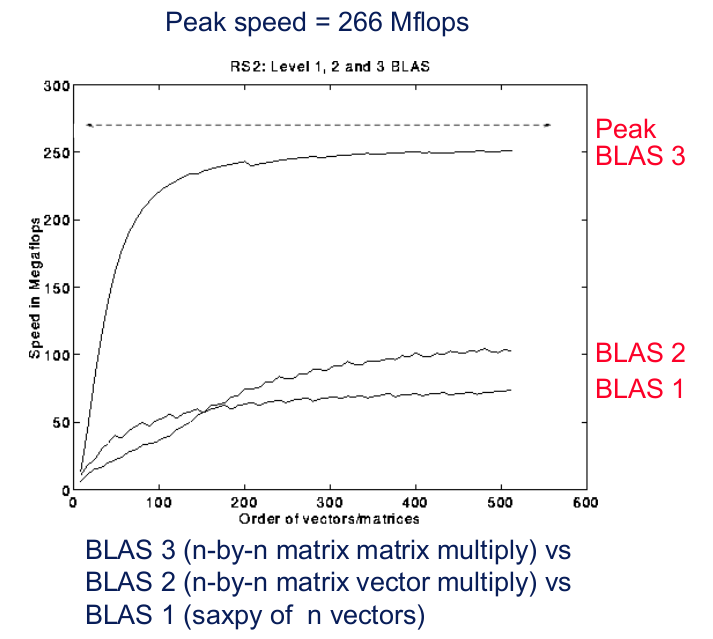
\includegraphics[width=12cm, height=8cm] {BLASSpeed}}
\caption{BLAS speeds.}
\label{fig:61}
\end{figure}    

Fabrikatzaile bakoitzak optimizatutako BLAS liburutegiak (AMD ACML,Intel MKL) dituzte eta beraz, multi-threaded dira.
Beste aukera bat, optimizatutako BLAS instalazioa ATLAS (Automatically Tuned Linear Algebra Software) bidez egitea.    

\subsubsection*{\textbf{LAPACK}}.

Zenbakizko algebra linealaren liburutegia da.

\begin{enumerate}
\item Sistema linealak: $AX=b$.
\item Least Square: choose $x$ to minimize $\|Ax-b\|$.
\item Eigenvalues.
\item Balio singularren deskonposaketa (SVD).
\end{enumerate}

Posible den guztietan, BLAS-3 funtzioetan oinarritzen da.


\subsection{Laburpena.}

Algoritmo bat inplementatzen dugunean kontutan hartu beharrekoa:

\begin{enumerate}

\item Lerro edo zutabe araberako iterazioak exekuzio denboran eragin handia du.

\item Kodea garbia eta ulergarria mantendu behar da.

\item Badaude kodearen exekuzio denboraren analisia egiteko tresnak (adibidez gprof). Algoritmoaren funtzio bakoitzaren exekuzio denborari buruzko informazio erabilgarria lortuko dugu. Zenbait gauza modu sinplean azkartu daitezke baina zenbait beste gauza azkartzeko esfuertzu handia eskatu dezake.

\item Optimizatutako beste hainbat kode erabiltzea komenigarria da. LAPACK aljebra lineal paketea Fortran eta C-lengoaitetatik deitu daiteke. Eraberean, LAPACKek BLAS subrutinak erabiltzen ditu.  Subrutinak hauek matrizen arteko biderketak, "inner product", ... BLAS konputagailu arkitektura ezberdinetarako optimizatutako bertsioak daude.
 


\end{enumerate}


\chapter{Review.}

\section{Sarrera.}

\section{Efemerideak.}

Hiru dira planetak efemerideak,

\begin{enumerate}
\item Jet Propulsion Laboratory, DE (Development Ephemerides).

      Integrazio tartea: $1550-2650$.

      Zenbkizko metodoa: "DIVA" (Krogh,1997).A variable order Adams method.
      
      Doitasuna: "QIVA" a quaruple precision of "DIVA" : the equations of motion , the newtonian part is computed in quadruple precision; all of the rest are computed in double precision.

\item Paris Observatory, INPOP (Intégrateur Númerique Planétaire de l'Observatoire de Paris).
      
      Integrazio tartea: .
      
	  Zenbakizko metodoa: The integrator is an Adams-Cowell method with fixed step-size.
	  
	  Doitasuna:  the programming is done in C language, thus allowing to use the extended precision (80 bits). 
	  Integrating in quadruple precision would of course reduce the round off error in a very large amount, but the
	  CPU time is about 15 time larger than for double precision arithmetic (or extended arithmetic) on our machine
	  (Itanium II with Intel C++ compiler). Nevertheless, it was possible to obtain an additional order of magnitude im-
	  provement by using a single addition in simulated quadruple precision in the corrector step with a very small over-
	  head.
	  
	  Hardware: Intel Itanium II processors.
	  
\item St. Petersburg, EPM (Ephemerides Planets-Moon).
      
      Integrazio tartea: .
      
      Zenbakizko metodoa: Everhart. Implicit RK method (Gauss-Radau).
      (An efficient integrator that uses Gauss-Radau Spacings)
      
      Doitasuna: double precision. The change of ERA system integrator (19 decimal digits instead of 15 ones) with the aim to reduce the round-off error. (Extended precision).
      
\end{enumerate}

\paragraph{Influence of the methods of constructing ephemerides...}
It is obvious that such ephemerides in themselves must have 128 bits, that is, comprise the coefficients calculated with quadruple precision.


\section{Eguzki-sistemaren integrazio luzeak.}

A.Morbidellik \cite{Morbidelli2002} eguzki-sistemaren zenbakizko integrazioen algoritmoen garapenaren azterketan, gaia hauek sailkatzen ditu:

\begin{enumerate}

\item The classical period.

$90$. hamarkada hasiera arte,  

\item The symplectic period.

\item The statistic period.

\item The planetary accretion period. 

\end{enumerate}


Wisdomek eta Holmanenek bere lanean \ycite[1991]{Sussman1992},  eguzki-sistemaren epe luzeko simulazioetarako integratzaile  sinplektikoen erabilerak arrakasta izan zuen. N-planeta eta masa nagusiko gorputza bat dugula kontsideratuta, problemaren Hamiltondarra bitan banatu zuten:  Hamiltondar Kleperiarra eta interakzioen Hamiltondarra. Metodo honetan, Hamiltondar bakoitzaren soluzioa tartekatuz, problema osoaren ebazpena kalkulatuko da. 

Wisdom eta Holmanen inplementazioak ez ditu kolisio gertuko egoerak onartzen. Arazo hau gainditzeko, urteetan zehar algoritmo honen hainbat aldaera proposatu dira: Levinson eta Duncan-ek \ycite[1994]{Levison1994}  \emph{SWIFT} softwarea garatu zuten;  Duncan, Levinson eta Lee-k \ycite[1998]{Duncan1998} \emph{SYMBA} softwarea garatu zuten; Chambers-ek \cite{Chambers1999} \emph{MERCURY} softwarea garatu zuen. Berriki, Hernandez eta Bertschinger-ek \ycite[2015]{Hernandez2015} garapen berri bat proposatu dute.

Koordenatu sistema aukera ezberdinak erabili dira Hamiltondarraren banaketa lortzeko. Jacobi koordenatuak eta koordenatu Heliozentrikoak erabili ohi dira bakoitzak bere abantaila eta desbaintailekin.

Problema integratzeko oinarrizko metodoa \emph{leapfrog} metodoa dugu. Metodo hau 2 ordeneko da. Orden altuagoko splitting eskemak : McLachlan \ycite[1995]{McLachlan1995}, Laskar eta Robutel \cite[2001]{Laskar2001}, Blanes \cite{Blanes2013}.

   
       

\part{Core}
\chapter{IRK: Puntu-Finkoa.}

\section{Sarrera.}

Gure helburua, biribiltze errore txikia duen IRK metodoaren inplementazioa proposatzea da. Integrazioaren exekuzio denborak onargarriak izan daitezen behartuta, honako aurrebaldintza finkatu dugu: ekuazio diferentzialaren eskuin aldeko funtzioaren 
sarrera eta irteera argumentuak makina zenbakiak izatea, hau da, konputagailuan Hardware bidezko exekuzioa (azkarra) duen koma-higikorrezko aritmetika erabiltzea. Gaur-egun, zientzia-konputazioan \it{double} ($64$ bit) koma-higikorrezko aritmetikarekin lan egiten da eta beraz, praktikan erabiltzaileak ekuazio diferentziala \it{double} datu-mota honetan zehaztuko duela suposatuko dugu.      

\paragraph*{} Lehenengo Hairer-en inplementazioa aztertuko dugu. Ondoren, IRK inplementazioa hobetzeko gure proposamenak azalduko ditugu. Azkenik, zenbakizko gure inplementazioaren emaitzak erakutsiko dugu.

\section{Hairer-en inplementazioa.}

Gure abiapuntua, Haierek \cite{Hairer2008} proposatutako inplementazio hartu dugu.  
Lan honetan, IRK metodo sinplektikoaren puntu-finkoaren inplementazio estandarraren biribiltze errorearen garapen okerraz jabetu ziren eta gainera, metodo sinplektiko esplizituetan agertzen ez zena. Hauen ustez, bi ziren errore honen jatorriak:

\begin{enumerate}
\item Integrazioan $a_{ij}, b_i \in \mathbb{R}$ koefiziente zehatzak erabili ordez, biribildutako $\tilde a_{ij},\tilde b_i \in \mathbb{F}$ erabiltzeak, aplikatutako IRK metodoa zehazki sinpletikoa ez izatea eragiten du.
\item Puntu-finkoaren geratze irizpide estandarra dela eta, urrats bakoitzean errore sistematikoa gertatzen da.
\end{enumerate}    

\paragraph*{}Arrazoi hauek aztertu ondoren, honako konponbideak proposatu zituzten:

\begin{enumerate}
\item Doitasun handiagoko koefizienteak erabili, hauetako bakoitza bi koma-higikorreko koefizienteen batura kontsideratuz $a_{ij}= a^{\ast}_{ij}+\tilde a_{ij}, \ b_i= b^{\ast}_i+\tilde b_i$.
\item Iterazioak geratu, definitutako norma txikitzeari uzten dionean.

\[\triangle ^{[k]} = \max_{i=1,\dots,s}\|Y_i^{[k]}-Y_i^{[k-1]}\|_{\infty} \]
\begin{equation*}
\triangle^{[k]} = 0 \ \ or \  \triangle^{[k]} \geqslant \triangle^{[k-1]}
\end{equation*}
  	 	
\end{enumerate}

Jarraian Hairer-en algoritmoa laburtuko dugu  (notazioa sinplifikatze aldera $Y_{n,i}$ gaiaren ordez, $Y_i$ adierazpena erabiliko dugu).

\begin{algorithm}[h]
 \BlankLine
  $e=0$\;
  \For{$n\leftarrow 1$ \KwTo $endstep$}
  {
   \BlankLine
   $k=0$\;
   Hasieratu  $Y_{i}^{[0]}$\; 
   \BlankLine
   \While{ ($\triangle^{[k]} \ != 0 \ \ and \  \triangle^{[k]} < \triangle^{[k-1]}) $}
   {
    \BlankLine 
    $k=k+1$\;
    $F_{i}^{[k]}=f(Y_{i}^{[k-1]}) $\;
    $Y_{i}^{[k]}=y_{n-1}+ h \ \big(\sum\limits_{j=1}^{s} a^{\ast}_{ij} F_{j}^{[k]} \big) 
                          + h \ \big(\sum\limits_{j=1}^{s} \tilde a_{ij} F_{j}^{[k]} \big)$\; 
    $\triangle ^{[k]} = \max_{i=1,\dots,s}\|Y_{i}^{[k]}-Y_{i}^{[k-1]}\|_{\infty}$\;
   }
   \BlankLine
    $\delta_{n}= \bigg(h \ \big(\sum\limits_{i=1}^{s} b^{\ast}_i F_{i}^{[k]} \big)
               + h \ \big(\sum\limits_{i=1}^{s} \tilde b_i F_{i}^{[k]} \big) \bigg)+e $\;
%    $\delta e=\delta_{n}+e $\;
    $y_n=y_{n-1}+\delta_n$\;
    $e=(y_{n-1}-y_n)+\delta_n$\;            
   \BlankLine
 }
 \caption{Main Algorithm}
\end{algorithm}


\section{Gure inplementazioa.}

IRK metodoaren puntu-finkoaren inplementazioan lau proposamen berri egin ditugu. Lehen bi proposamenak  Hairer-ek bere lanean proposatutako konponbideen hobekuntzak dira. Batetik, IRK-ren birformulazio bat erabiliz, IRK metodoaren koma-higikorrezko koefizienteak sinplektizidade baldintza zehazki betetzea lortuko dugu. Bestetik, geratze irizpidean arazo batzuk topatu ditugu eta arazo hauek gainditzen dituen geratze irizpide sendoagoa garatu dugu. Beste bi proposamenak dagokionez, bata batura-konpensatuari erlazionatuta dago eta bestea biribiltze errorea monitorizatzeko proposamena da.
\paragraph*{} Bestalde kapitulu honen bukaeran, batetik interpolazio bidezko atalen hasieraketa eta bestetik, Gauss-Seidel moduko puntu-finkoaren iterazioak azaldu ditugu. Bukatzeko, gure algoritmoa azalduko dugu.  

\subsection{Koefizienteak (1.proposamena).}

IRK metodoa definitzen duten $a_{ij},b_i$ koefizienteak, biribildutako $\tilde a_{ij},\tilde b_i \in \mathbb{F}$ ordezkatzerakoan, sinpletizide baldintza ez da beteko,
\begin{equation} \label{eq:61}
b_{i}a_{ij}+b_{j}a_{ji}-b_{i}b_{j}=0, \ \ 1 \leqslant i,j \leqslant s.
\end{equation}  
  
Arazo hau gainditzeko asmoarekin, IRK metodoa era honetan birformulatuko dugu,

\begin{equation}
\label{eq:62}
Y_{n,i}=y_n+ \sum\limits_{j=1}^{s} \mu_{ij} L_{n,j},  \ \ L_{n,i}=hb_if(Y_{n,i})
\end{equation}

\begin{equation}
\label{eq:63}
y_{n+1}=y_n+\sum\limits_{i=1}^{s} L_{n,i}
\end{equation}

non 

\begin{equation*}
\mu_{ij}=\frac{a_{ij}}{b_j}, \ \ 1 \le i,j \le s.
\end{equation*}

Eta sinplekzidade baldintza modu honetan berridatziko dugu,

\begin{equation}
\mu_{ij}+\mu_{ji}-1=0, \ \ \ 1 \le i,j \le s.
\end{equation}

\paragraph*{} Formulazio honek  estandarrarekiko duen abantaila handiena , sinplektizidade baldintzan biderketarik agertzen ez denez,  baldintza hau betetzen duten $\tilde \mu_{ij} \in \mathbb{F}$ koefizienteak aurkitzeko bidea errazten zaigu. Zehazki era honetan finkatuko ditugu gure koefizienteak:

\begin{enumerate}
\item $\mu_{ij}$ koefizienteak.\\

Batetik $s$-ataleko Gauss metodoetan, $\tilde \mu_{ii}:=\frac{1}{2}, \ i=1,\dots,s$. Bigarrenik $\tilde \mu_{ij}:=fl(\mu_{ij}), \ 1 \le j < i \le s$ finkatuko dugu. Azkenik $\frac{1}{2} < |\mu_{ij}| <2$ denez, eta Sterbenz-en Teoremaren (ikus. \ref{eq:4311}) arabera  $\tilde \mu_{ji}:=1-\tilde{\mu_{ij}}$ koma-higikorrezko adierazpen zehatza du. Ondorioz, simplektizitate baldintza zehazki betetzen duten koma-higikorrezko $\tilde \mu_{ij}$ koefizienteak lortu ditugu.   

\begin{equation}
\left(\begin{array}{cccc}
    \frac{1}{2}       & 1-fl(\mu_{21}) & \dots & 1-fl(\mu_{s1})      \\
    fl(\mu_{21})      & \frac{1}{2}    & \dots & 1-fl(\mu_{s2})      \\
    \vdots            & \ddots         &       & \vdots              \\
    fl(\mu_{s1})      & fl(\mu_{s2})   & \dots & \frac{1}{2}          \\ 
     \end{array}\right)
\end{equation}

\item $b_{i}$ koefizienteak.\\

Gure inplementazioan, $hbi$ koefizienteak erabiliko ditugu. Batetik, koefiziente hauek simetrikoak direla eta bestetik, $\sum\limits_{i=1}^{s} hb_i=h$ berdintza bete behar dela kontutan hartuz,

\begin{eqnarray}
hb_1=hb_s:= h - \sum\limits_{i=2}^{s-1} hb_i
\end{eqnarray}


\end{enumerate}

\subsection{Geratze irizpidea (2.proposamena).}

Ekuazio inplizituaren (\ref{eq:62}) soluzioaren hurbilpena lortzeko puntu-finkoko iterazioa era honetan definituko dugu. Iterazioaren abiapuntua $Y_i^{[0]}$  finkatu eta $k=1,2,\dots$ iterazioetarako $Y_i^{[k]}$ hurbilpenak lortu dagokigun geratze irizpidea bete arte.

\begin{equation}
L_i^{[k]}=hb_if(Y_i^{[k-1]}), \ \ Y_i^{[k]}=y_n+\sum\limits_{j=1}^{s} \mu_{ij} L_j^{[k]}
\end{equation}
 
\paragraph*{}IRK metodoaren inplementazio estandarrean geratze erizpidea honakoa da,

\begin{equation*}
\triangle^{[k]}=(Y_1^{[k]}-Y_1^{[k-1]},\dots,Y_s^{[k]}-Y_s^{[k-1]}) \in \mathbb{R}^{sd},
\end{equation*}
 
\begin{equation}
\|\triangle^{[k]}\| \le tol
\end{equation}
non $\|.\|$ aurre-finkatutako bektore norma eta \emph{tol} tolerantzia errorea den . Tolerantzia txikiegia aukeratzen bada, gerta daiteke tolerantzia hori ez lortzea eta infinituki iterazioak exekutatzea. Baina tolerantzia ez bada behar adina txikia  aukeratzen, iterazioak puntu-finkora iritsi aurretik geratuko dira eta lortutako $Y_i^{[k]}$ hurbilpenak biribiltze errorea baino errore handiago izango du.

\paragraph*{} Gogoratuz Hairer-ek proposatu zuen geratze irizpidea :  $\triangle^{[k]} = 0$ (puntu-finkora iritsi delako) ;  edo   $\triangle^{[k]} \geqslant \triangle^{[k-1]}$ (biribiltze errorea nagusi delako). Orokorrean, geratze irizpide honek ondo funtzionatzen du baina batzuetan, iterazioak goizegi geratu direla konprobatu dugu. Gure iritziz, honen arrazoia da $\triangle^{[k]} \geqslant \triangle^{[k-1]}$ biribiltze errorea nagusia dela adierazten duen arren, badago $j \in \{1,\dots,sd\}$ osagairik,   $|\triangle_j^{[k]}| < |\triangle_j^{[k-1]}|$ hobetzeko tartea duena. 

\paragraph*{} Gure proposamena azaldutako arazoari soluzioa emateko asmoarekin, iterazioak jarraitzea honako baldintza betetzen ez den bitartean,

\begin{equation}
\exists j \in \{1,\dots,sd\} \ , \ |\triangle_j^{[1]}| >|\triangle_j^{[2]|}>\dots>|\triangle_j^{[k]}|>0.
\end{equation}


\subsection{Batura konpensatua (3.proposamena).}

Integrazioaren zenbakizko soluzioa  $y_n \approx y(t_n)$ ($n=1,2,\dots$) lortzeko, urrats bakoitzean honako batura dugu,
\begin{equation*}
y_n=y_{n-1} + \phi(y_{n-1,h}).
\end{equation*}   

\paragraph*{} IRK metodoetan, $\phi: \mathbb{R}^{[d+1]} \rightarrow \mathbb{R}^d$ gehikuntza,
\begin{equation*}
\phi(y_{n,h})=\sum\limits_{i=1}^{s} L_{n,i},
\end{equation*}

\paragraph*{} non $L_{n,i}$ ($i=1,\dots,s$) inplizituki definitzen diren.

\paragraph*{} Urrats askotako integrazioetan, batura honetan gertatutako biribiltze erroreak doitasun galera garrantzitsua sortzen du. Beraz, zenbakizko integrazioetan biribiltze errorea gutxitzeko oso erabilgarria zaigu batura konpensatu teknika aplikatzea.

\begin{algorithm}[h]
 \BlankLine
  $\tilde {e}_0=0$\;
  \BlankLine
  \For{$n\leftarrow 1$ \KwTo $endstep$}
  {
   $\dots$\;
   \BlankLine
    $\tilde {\delta}_{n}= (\sum\limits_{i=1}^{s} L_{i}^{[k]}) \oplus \tilde {e}_{n-1} $\;
    $\tilde {y}_n=\tilde{y}_{n-1} \oplus \tilde{\delta}_n$\;
    $\tilde {e}_{n}=(\tilde{y}_{n-1} \ominus \tilde{y}_n)\oplus \tilde{\delta}_n$\;            
   \BlankLine
 }
 \caption{Batura konpensatua}
\end{algorithm}

\paragraph*{} $y_n \in \mathbb{R}^{d}$,  $y_n=\tilde y_{n-1}+\tilde \delta_n$ soluzioa zehatza izanik eta $\tilde y_n \in \mathbb{F}^{d}$,  $\tilde y_n=\tilde y_{n-1} \oplus \tilde \delta_n$ koma-higikorreko hurbilpena izanik, lortutako errore estimazioa $\tilde{e_n}$ ,  zehazki benetako biribiltze errorea da,

\begin{equation}
y_n=\tilde {y}_n+\tilde {e}_n. 
\end{equation}

\paragraph*{} Horregatik, IRK metodoaren inplementazioan, inplizituki $Y_{n,i}$ atalak askatzeko ekuazioetan, $\tilde {y}_n$ ordez ($\tilde{y}_n \oplus \tilde{e}_n$) erabiltzea proposatzen dugu,   

\begin{equation}
L_i^{[k]}=hb_if(Y_i^{[k-1]}), \ \ Y_i^{[k]}=\tilde{y}_n \oplus \big(\tilde{e}_n \oplus \sum\limits_{j=1}^{s} \mu_{ij} L_j^{[k]}\big).
\end{equation}

\paragraph{}Aldaketa honekin, lortutako zenbakizko soluzioaren doitasuna pixka bat hobetzea espero dugu. 


\subsection{Biribiltze errorearen estimazioa (4.proposamena).}

Zenbakizko integrazioaren biribiltze errorearen estimazioa, bigarren zenbakizko integrazio baten soluzioaren diferentzia gisa kalkulatuko dugu. Bigarren integrazio honetan, $Y_i^{[k]}$ atalak mantisa txikiagoko zenbakitara biribiltzen ditugu eta horrela doitasun gutxiagoko soluzioa lortzen dugu. 

$r\ge0$ zenbaki osoa, eta $x \in \mathbb{F}$ ($m$ doitasunezko koma-higikorrezko zenbakia) izanik, honako funtzioa definituko dugu,\\

\begin{algorithm}[H]
  \SetAlgoLined\DontPrintSemicolon
  \SetKwFunction{algo}{algo}\SetKwFunction{floatR}{floatR}
  \SetKwProg{myalg}{Algorithm}{}{}
  \SetKwProg{myproc}{Function}{}{}
  \myproc{\floatR {x,r}}{
    $res=(2^r x \oplus x)\ominus 2^r x$\;
    \KwRet res \;}
  \caption{floatR}
\end{algorithm} 

\paragraph*{}Funtzio honek itzultzen duen balioa, $(m-r)$ doitasunezko koma-higikorrezko zenbakia da. Beste modu batera esanda, $m$ biteko koma-higikorrezko $x$ zenbakiaren azken $r$ bitak zeroan jartzen dituen funtzioa.
     
\paragraph*{} $r<m$ zenbaki osoa finkatuta, bigarren integrazioaren puntu-finkoaren iterazioa honela kalkulatuko dugu,

\begin{equation}
L_i^{[k]}=hb_if(Y_i^{[k-1]}), \ \ Y_i^{[k]}=floatR\bigg(\tilde{y}_n \oplus \big(\tilde{e}_n \oplus \sum\limits_{j=1}^{s} \mu_{ij} L_j^{[k]}\big),r\bigg).
\end{equation}

Biribiltze errorearen estimazioa, zenbakizko soluzio nagusiaren $(y^{[main]}_n+e^{[main]}_n)$ eta $r$ balio txiki baterako (adibidez $r=3$) kalkulatutako bigarren zenbakizko soluzioaren $(y^{[sub]}_n+e^{[sub]}_n)$ arteko diferentzia bezala kalkulatuko dugu.  

\begin{equation}
estimazioa_n=(y^{[main]}_n+e^{[main]}_n)-(y^{[sub]}_n+e^{[sub]}_n)
\end{equation}

Gure algoritmoan estimazioa zuzenean lortzeko, bi integrazioak modu eraginkorrean kalkulatzen dira. Urrats bakoitzean, bi integrazioen $Y_i$ ($i=1,\dots,s$) ataletako balioak, biribiltze errorea estimazio handiegia ez den artean,  antzekoak mantentzen dira. Beraz, bigarren integrazioaren iterazio kopuru txikia beharko dugu, lehen integrazioaren bukaerako $Y_i$ ($i=1,\dots,s$) atalen balioak, bigarren integrazioaren $Y_i^{[0]}$ (i = 1, . . . , s) atalen hasieratzeko erabiliz (algoritmoa zehaztu ???).  


\begin{algorithm}[h]
  \BlankLine
  \For{$n\leftarrow 1$ \KwTo $endstep$}
  {
    \BlankLine
    $Y_n^{[0]}=G(Y_{n-1},h)$\;
    $\dots$\;
    $y_{n+1}=y_{n}+\delta_n$\;
    \BlankLine
    \BlankLine
    \eIf{$(initwithfirst)$}
    {$\hat{Y}_{n}^{[0]}=Y_{n}+(\hat{y}_n-y_n)$\;}
    {$\hat{Y}_{n}^{[0]}=G(\hat{Y}_{n-1},,h)$\;}
    $\dots$\;
    $\hat{y}_{n+1}=\hat{y}_{n}+\hat{\delta}_n$\;
    \BlankLine
    \BlankLine
    $estimation_n=(y_n+e_n)-(\hat{y}_n-\hat{e}_n)$\;
    \BlankLine
   }
 \caption{RKG2: errore estimazioa}
\end{algorithm}

\subsection{Atalen hasieraketa.} 

Ideia da, aurreko urratseko uneetako, $(t_{n-1}+hc_i,Y_{n-1,i}), \ i=1,\dots,s$ eta $(t_{n-1}+h,y_{n})$, balioei dagokien polinomio interpolatzailea erabiliz, urrats berriaren atalen hasieraketa  $(t_{n}+hc_i,Y_{n,i}^{[0]}), \ i=1,\dots,s$ kalkulatzea. 

\begin{figure}[h]
\centerline{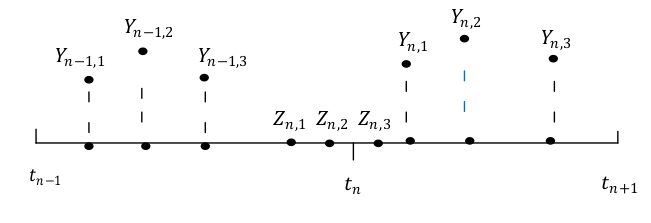
\includegraphics[width=12cm, height=4cm] {Interpolazioa}}
\caption{Interpolazioa.}
\label{fig:bost}
\end{figure}

\paragraph*{}($n-1$) urratseko informazioa erabiliz,
\begin{equation*}
Y_{n-1,i}=y_{n-1}+h \sum\limits_{j=1}^{s} a_{ij} f(Y_{n-1,j})
\end{equation*}

\begin{equation*}
y_n=y_{n-1}+h \sum\limits_{j=1}^{s} b_j f(Y_{n-1,j})
\end{equation*}

\begin{equation}
Y_{n-1,i}=y_n+h \sum\limits_{j=1}^{s} (a_{ij}-b_j) f(Y_{n-1,j})
\end{equation}

\paragraph*{}Dagokion polinomio interpolatzailea,

\begin{equation*}
P(t)=  l_1(t) Y_{n-1,1}+\dots+l_s(t) Y_{n-1,s}+l_{s+1}(t) y_n
\end{equation*}
  
\paragraph*{}non $l_i(t)$ Lagrangiar polinomioa dugu,
\begin{equation*}
 l_i(t)=\prod_{l\neq i,l=1}^{s+1} \frac{(t-(t_{n-1}+hc_l))}{(c_i-c_l)}, \ \ c_{s+1}=1.
\end{equation*}

\paragraph*{}Eta beraz,

\begin{equation}
Y_{n,i} \approx Y_{n,i}^{[0]}= P(t_n+hc_i) = y_n+ h \sum\limits_{j=1}^{s} \lambda_{ij}f(Y_{n-1,j})
\end{equation}

\paragraph*{} Modu honetan s-ataletako IRK metodo bakoitzari dagokion $\lambda_{ij}$ koefiziente interpolatzaileak lortu daitezke. Polinomio interpolatzailearen bidezko hasieraketa ona izango da, emandako urratsa ez bada oso handia eta problema stiff ez denean. Era berean aipatu nahi genuke, atal askotako metodoetan (adibidez $s=16$)  interpolaziozko koefizienteen kalkuluan ezabapen arazoak,  doitasun handian lan egitea behartzen gaituela interpolaziozko hasieraketa ona izateko.  

\subsection{Gauss-Seidel.}

\subsection{Algoritmoa.}

\paragraph*{} Formulazio berriari dagokion algoritmo orokorra,

\begin{algorithm}[H]
 \BlankLine
  $e=0$\;
  \For{$n\leftarrow 1$ \KwTo $endstep$}
  {
   \BlankLine
   Hasieratu  $Y_{i,n}^{[0]} \ \ , \ \ i=1,\dots,s $\;
   \BlankLine
   \While{ (konbergentzia lortu)}
   {
    \BlankLine 
    $L_{n,i}=hb_if(Y_{n,i}) \ \ , \ \  i=1,\dots,s$\;
    $Y_{n,i}=y_{n-1}+ \ \sum\limits_{j=1}^{s} \mu_{ij} L_{n,j}  \ \ , \ \  i=1,\dots,s$\;  
   }
   \BlankLine
    $\delta_{n}= \sum\limits_{i=1}^{s} L_{n,i}+e $\;
    $y_{n}=y_{n-1}+ \delta_{n} $\;
    $e=(y_{n-1}-y_n)+\delta_n$\;
   \BlankLine
 }
 \caption{Main Algorithm}
\end{algorithm}


\paragraph*{} Eta puntu-finkoa erabiliz,

\begin{algorithm}[H]
 \BlankLine
  $e=0$\;
  \For{$n\leftarrow 1$ \KwTo $endstep$}
  {
   \BlankLine
   $k=0$\;
   Hasieratu  $Y_{i}^{[0]}$\;
   \BlankLine
   \While{ (konbergentzia lortu)}
   {
    \BlankLine 
    $k=k+1$\;
    $L_{i}^{[k]}=hb_if(Y_{i}^{[k-1]}) $\;
    $Y_{i}^{[k]}=y_{n-1} + \ \big(e+\sum\limits_{j=1}^{s} \mu_{ij} L_{j}^{[k]}\big)  $\;  
   }
   \BlankLine
    $\delta_{n}= \sum\limits_{i=1}^{s} L_{i}^{[k]}+e $\;
    $y_{n}=y_{n-1}+ \delta_{n} $\;
    $e=(y_{n-1}-y_n)+\delta_n$\;
   \BlankLine
 }
 \caption{Main Algorithm}
\end{algorithm}


\section{Esperimentuak.}

Biribiltze erroreari dagokionez gure inplementazioa optimotik gertu dagoela erakutsi nahi dugu. Esperimentuetan lau integrazio mota egingo ditugu:

\begin{enumerate}

\item Quadruple doitasuna. Zenbakizko integrazio hau soluzio zehatza kontsideratuko dugu eta errore globala kalkulatzeko erreferentziazko soluzioa izango da.

\item Integrazio optimoa (ideala). Ekuazio diferentzialaren eskuin aldeko funtzioaren ebaluazioa ezik, konputazioa doitasun quadruplean  egiten duen inplementazioa. 

\item Double doitasuna.

\item Double doitasuna (klasikoa.)

\end{enumerate}

\subsection{Doitasun azterketa.}

Integrazio bakarra egin ordez, perturbatutako $P=100$ hasierako balioekin zenbakizko integrazioak exekutatu ditugu eta emaitza guzti hauen batezbestekoan oinarritu gara, biribiltze errorearen azterketa egokia egiteko.    

\paragraph*{}  $ k. \ (1,\dots,P)$ integrazio bakoitzean $N$ urrats eman baditugu, $t_i=t_0+i*h, \ i=1,\dots,N$ uneetarako lortuko dugu 
zenbakizko soluzioa,
\begin{equation*}
(q_i^{[k]},p_i^{[k]})\approx(q(t_i)^{[k]},p(t_i)^{[k]}).
\end{equation*}

\paragraph*{}Sistema Hamiltondarretan energia kontserbatzen da eta  definizioa hau izanik $H(q(t),p(t))=E(t)$,
\begin{equation*}
E_i^{[k]}=H(q_i^{[k]},p_i^{[k]}).
\end{equation*}

\begin{enumerate}

           \item Energia errorea.\\
           \begin{equation*}
           \triangle E_i^{[k]}=\frac{(E^{[k]}_i-E^{[k]}_0)}{E^{[k]}_0}, \ \ i=1,\dots,N \ eta \ k=1,\dots,P.
           \end{equation*}  
           
           \begin{equation*}
           \bar{\triangle E_i}=\frac{1}{P} \sum_{k=1}^{P} \triangle E_i^{[k]}, \ \ i=1,\dots,N.
           \end{equation*}
           
           \begin{equation*}
           \sigma_i=\sqrt{\frac{1}{P} \sum_{k=1}^{P} (\triangle E_i^{[k]})^2-(\bar{\triangle E_i})^2}, \ \ i=1,\dots,N.
           \end{equation*}
           
           \begin{equation*}
           \bar{MaxE}=\max_{i=1,\dots,N} |\bar{\triangle E_i}|
           \end{equation*}

           \item Energia errore lokala.\\ 
            $P=100$ integrazio guztietarako, bi urratsen arteko energia lokalaren batazbestekoa ($\mu$) eta desbiazio estarrada ($\sigma$). 
            
           \begin{equation*}
             \blacktriangle E_i^{[k]}=\frac{(E^{[k]}_i-E^{[k]}_{i-1})}{E^{[k]}_0},\ \ \ i=1,\dots,N \ eta \ k=1,\dots,P.          
           \end{equation*}
           
           \begin{equation*}
            \bar{\mu}= \frac{1}{N\cdot P} \bigg(\sum_{k=1}^{P} \sum_{i=1}^{N} {\blacktriangle E_i^{[k]}\bigg)}, \ \
            \bar{\sigma} = \sqrt{\frac{1}{N\cdot P} \bigg(\sum_{k=1}^{P} \sum_{i=1}^{N} {(\blacktriangle E_i^{[k]}-\bar{\mu)}^2}\bigg)}
           \end{equation*}
           
           \item Errore Globala ($\bar{Ge}$).\\
            Doitasun laukoitzean lortutako soluzioari soluzio zehatza deituko dugu,
            
            \begin{equation*}
            yexact^{[k]}_i=\tilde{y}^{[k]}_i=(\tilde{q}^{[k]}_i,\tilde{p}^{[k]}_i)
            \end{equation*}

            eta $k.$ soluzioari dagokion errorea, 
            
            \begin{equation*}
            Ge^{[k]}_i=\|\tilde{q}^{[k]}_i-q^{[k]}_i\|
            \end{equation*}
            
            \begin{equation*}
            \bar{Ge_i}= (\frac{1}{P}\sum_{k=1}^{P} Ge^{[k]}_i) \ , \
                          \bar{MaxGe}=\max_{i=1,\dots,N} (\bar{Ge_i})
            \end{equation*}           
           
            \item Puntu-finkoa lortutako urratsen portzentaia ($\bar{\triangle}0$).\\
           
            $\triangle0^{[k]}$,  $k.$ integrazioan puntu-finkoa lortutako urratsen portzentaia izanik,
            
            \begin{equation*}
            \bar{\triangle}0= \frac{1}{p}\sum_{k=1}^{p}\triangle0^{[k]}
            \end{equation*}
 
            \item Errore estimazioa ($\bar{\mu Q_i}$ , $\bar{\sigma Q_i}$). \\
            
            Lehenengo estimazioa honela definituko dugu,
            \begin{equation*}
            Est^{[k]}_i=\|{q}^{[k]}_{main_i}-q^{[k]}_{sub_i}\|.
            \end{equation*}

            
            Errore estimazioaren kalitatea neurtzeko,
            \begin{equation} \label{eq:eq_Qi}
               Q_i^{[k]}=\log_{10} \bigg(\frac{Est^{[k]}_i}{Ge^{[k]}_i}\bigg)
            \end{equation}
            \[\bar{\mu Q_i}=\frac{1}{P}\sum_{k=1}^{p} Q_i^{[k]} \ , \ 
              \bar{\sigma Q_i}=\sqrt{\frac{1}{P}\sum_{k=1}^{P} (Q_i^{[k]}-\bar{\mu Q_i})^2}\]
\end{enumerate} 

\subsection{Brouwer legea.}

In order to test the randomness of numerical error (not systematic) in the integration, some researches verify that the method achieves Brouwer's law \cite{Brouwer1937}. Denote by $\epsilon_{n}$ the error contribution over one step in the Hamiltonian H(y),

Zenbakizko integrazioaren errorea hausazkoa dela ziurtatzeko, metodoak Broweren legea \cite{Brouwer1937} duela konprobatu ohi izan da. Urrats batean $H(y)$ Hamiltondarrean egindako errorea $\epsilon_{n}$ deituko diogu,

\begin{equation} \label{eq:18}
H(y_{n+1})-H(y_{n})=\epsilon_{n}.
\end{equation}

Batezbestekoa zero eta bariantza, biribiltze errorearen karratuaren ($u^2=(2^{-m})^2$) proportzionala duen hausazko aldagaia dela kontsideratuz, 
Brouwer legearen arabera, energia-errorea ...

and assuming it is a random variable with mean zero and variance proportional to the square of the round-off unit, Brouwer's law says that error of first integrals conservations due to round-off will grow like the square-root of time. See also Hairer \cite{Hairer2006}[VIII.5]. Figure \ref{fig:brouwer103} plots the histogram of the Local energy error against the normal distribution $N(\mu, \delta)$.

\subsection{Pendulu bikoitza.}

\begin{table} [h]
\caption{Summary of Non-Chaotic case.}
\label{tab:2}       % Give a unique label
\begin{tabular}{c|c c c c c} 
 Arithmetic   &  $\bar{\triangle}0$  &  $\bar{MaxE}$ & $\bar{\mu}$  & $\bar{\sigma}$   & $\bar{MaxGe}$  \\
                           &   \%            &       &          &            &         \\
 \hline
                           &                 &         &       &           &          \\
 Quadruple prec            &   $93.6$        &  $3e10^{-19}$  & $3e10^{-29}$  & $2e10^{-20}$  &      \\	    
 Ideal Integrator          &   $98.3$        &  $9e10^{-16}$  & $2e10^{-19}$  & $8e10^{-18}$ &  $4e10^{-12}$\\
 Double prec               &   $94.8$        &  $2e10^{-15}$  & $4e10^{-19}$  & $8e10^{-18}$ &  $6e10^{-12}$\\
\end{tabular}
\end{table}

\begin{table} [h]
\caption{Summary of Chaotic case.}
\label{tab:3}       % Give a unique label
\begin{tabular}{c|c c c c c} 
 Arithmetic   &  $\bar{\triangle}0$  &  $\bar{MaxE}$ & $\bar{\mu}$  & $\bar{\sigma}$   & $\bar{MaxGe}$  \\
                           &   \%            &       &          &            &         \\
 \hline
                         &                 &         &       &             \\
 Quadruple prec          &   $93.6$        &  $2e10^{-19}$  & $7e10^{-22}$ & $1e10^{-20}$    &          \\	    
 Ideal Integrator        &   $98.3$        &  $3e10^{-16}$  & $1e10^{-18}$  & $9e10^{-18}$   & $0.18$    \\
 Double prec             &   $94.7$        &  $3e10^{-16}$  & $1e10^{-18}$  & $1e10^{-17}$   & $0.23$    \\
\end{tabular}
\end{table}

\begin{figure}[h]
\centering
\subfloat[Non chaotic: energy error.]{
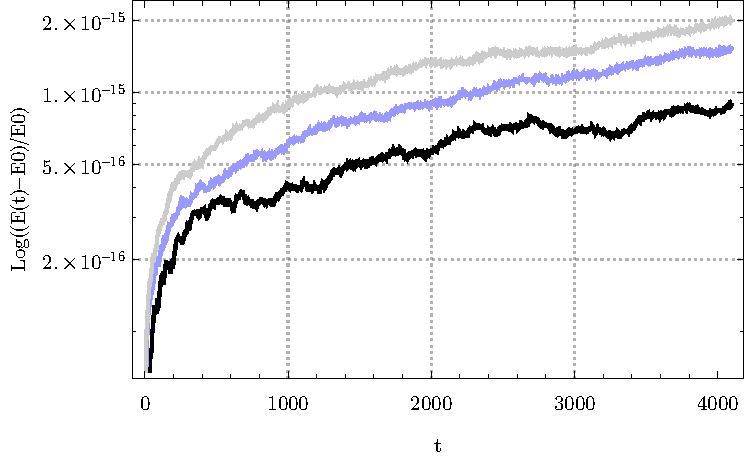
\includegraphics[width=.500\textwidth]{plot3a}
}
\subfloat[Non chaotic: global error.]{
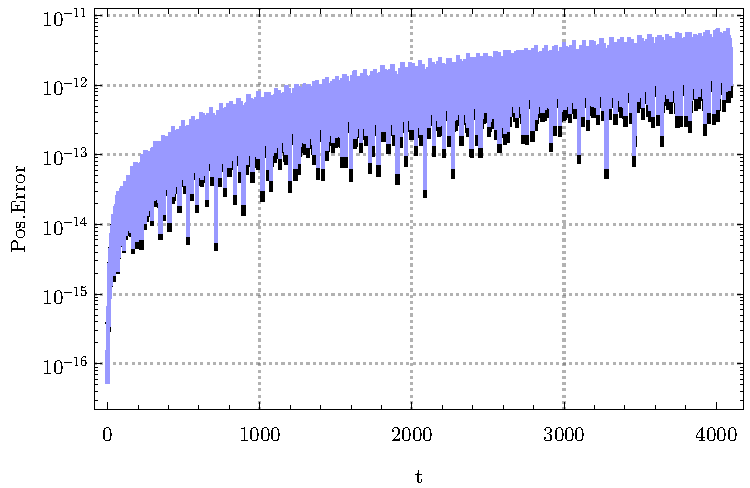
\includegraphics[width=.500\textwidth]{plot3b}
}
\vskip\baselineskip
\subfloat[Chaotic: energy error.]{
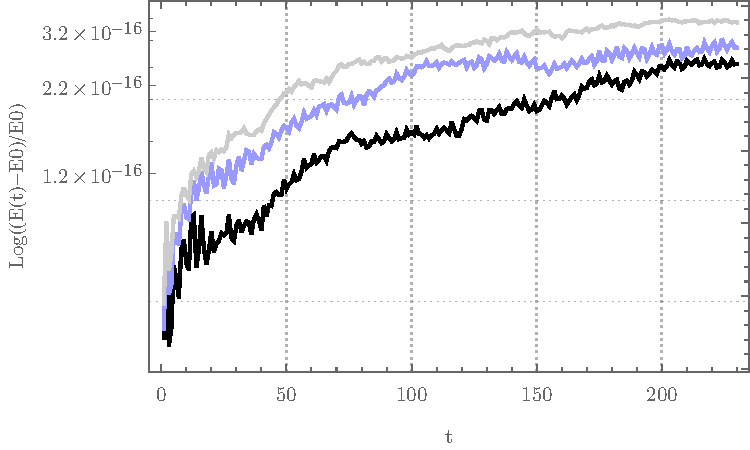
\includegraphics[width=.500\textwidth]{plot3c}
}
\subfloat[Chaotic: global error.]{
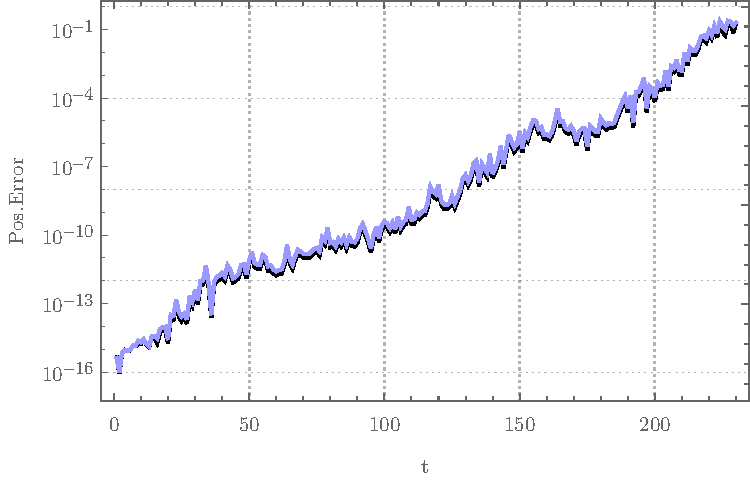
\includegraphics[width=.500\textwidth]{plot3d}
}
\caption{\small We show Non-Chaotic case (a,b) and Chaotic case (c,d). Left figure mean energy error evolution $\bar{\triangle E_i}$ and right figure mean Global error evolution $\bar{Ge_i}$ of the 100 integrations for \textit {Ideal Integrator} (black) , \textit {Double prec} (blue) and \textit {Classic Implementation} (gray).}
\label{fig:plot3}
\end{figure}

\subsection*{Brouwer-legea.}


\begin{figure}[h]
\centering
\subfloat[Non-Chaotic: Ideal.]{
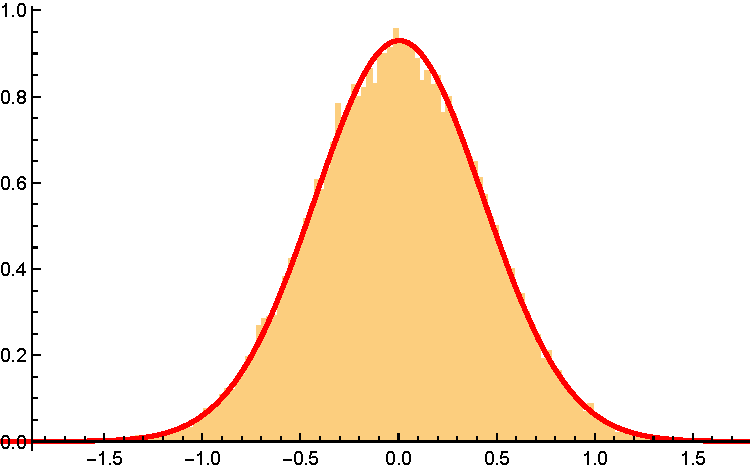
\includegraphics[width=.450\textwidth]{brouwer4a}
}
\subfloat[Non-Chaotic: rdigits=0.]{
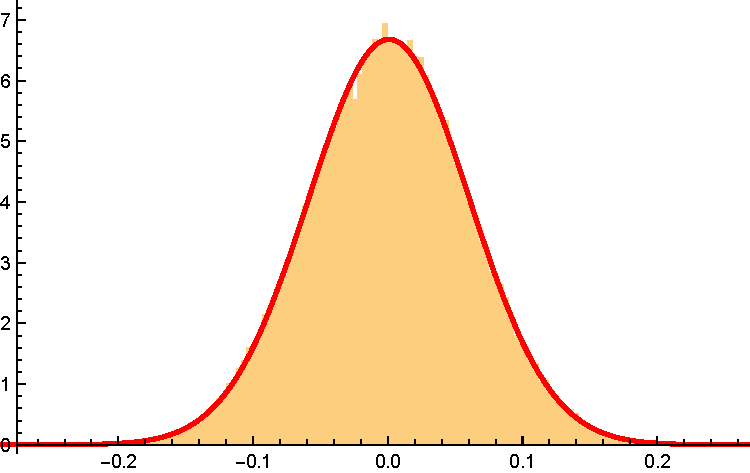
\includegraphics[width=.450\textwidth]{brouwer4b}
}
\vskip\baselineskip
\subfloat[Chaotic: Ideal.]{
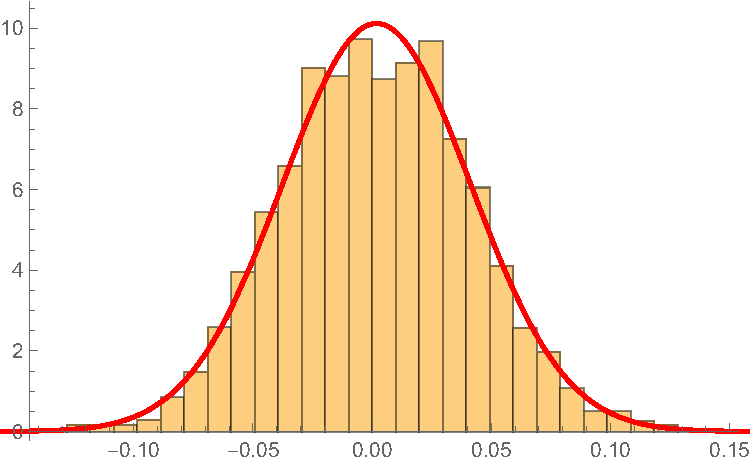
\includegraphics[width=.450\textwidth]{brouwer4c}
}
\subfloat[Chaotic: rdigits=0.]{
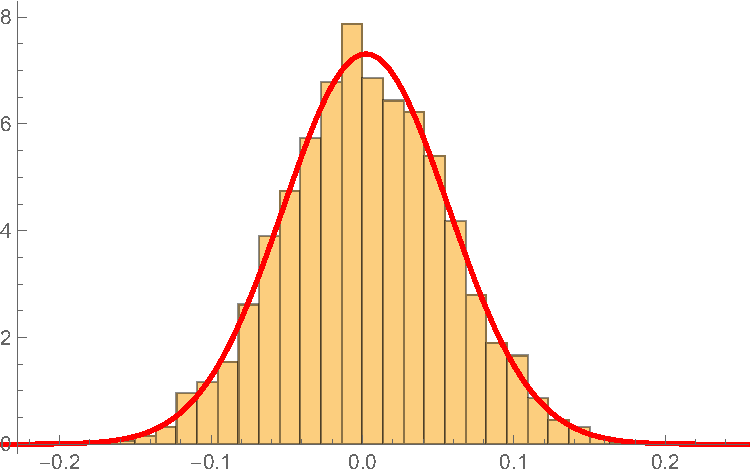
\includegraphics[width=.450\textwidth]{brouwer4d}
}
\caption{ \small Histogram of energy errors for Non-Chaotic case (a,b) and for Chaotic case (c,d).}
\label{fig:brouwer103}
\end{figure}

\subsection*{Biribiltze erroreaen estimazioa.}


\begin{figure}[h]
\centering
\subfloat[Non Chaotic: estimation]{
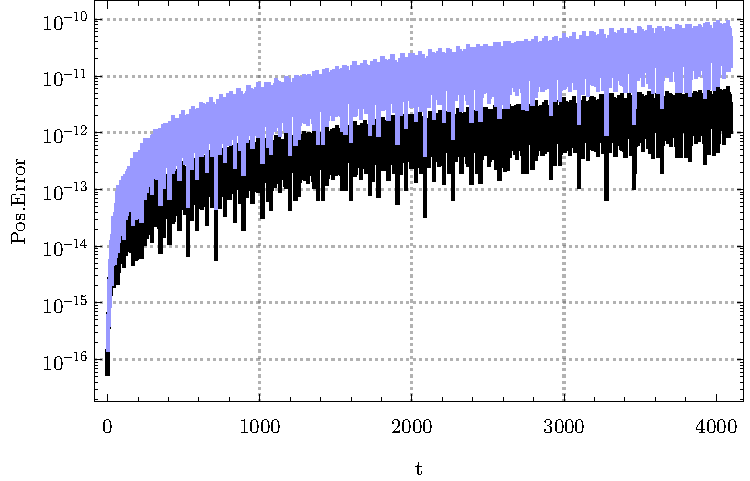
\includegraphics[width=.500\textwidth]{plot5a}
}
\subfloat[Non Chaotic: quality of estimation]{
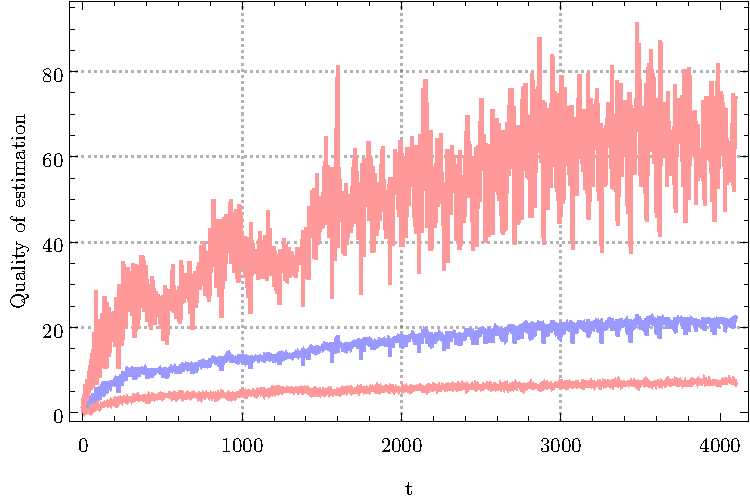
\includegraphics[width=.500\textwidth]{plot5b} 
}
\vskip\baselineskip
\subfloat[Chaotic: estimation]{
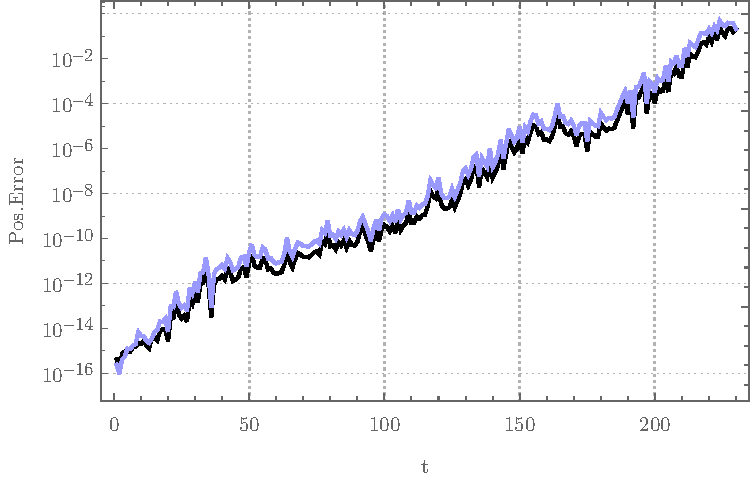
\includegraphics[width=.500\textwidth]{plot5c} 
}
\subfloat[Chaotic: quality of estimation]{
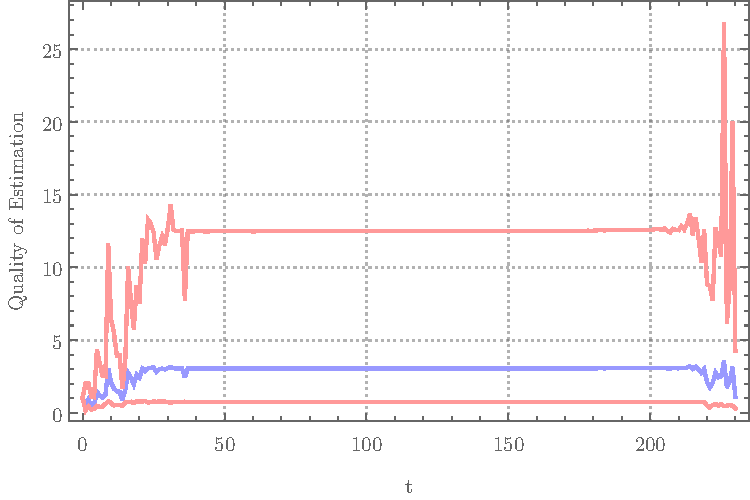
\includegraphics[width=.500\textwidth]{plot5d}
}

\caption{\small Estimation round-off error. We compare evolution of our estimation error (blue) with evolution of global error (black). Estimation Quality. We show mean (blue) and  standard deviation (red) of the quality according our definition of (\ref{eq:eq_Qi}).}
\label{fig:plotest}
\end{figure}

\subsection{N-Body problema.}


\begin{figure}[h]
\centering
\subfloat[Energy error.]{
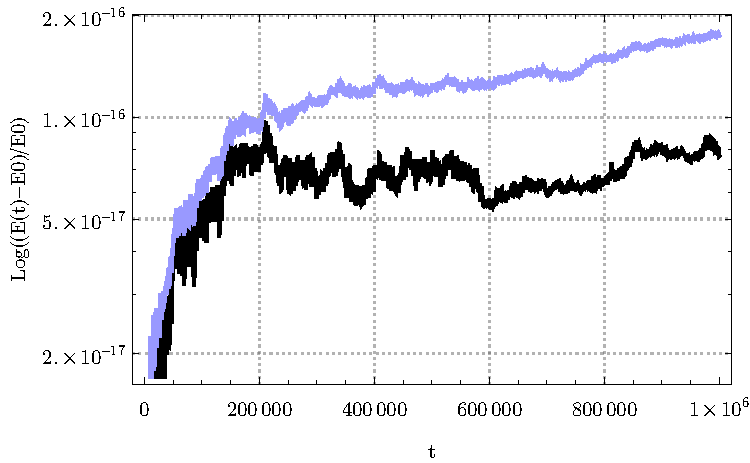
\includegraphics[width=.500\textwidth]{plot6a}
}
\subfloat[Global error.]{
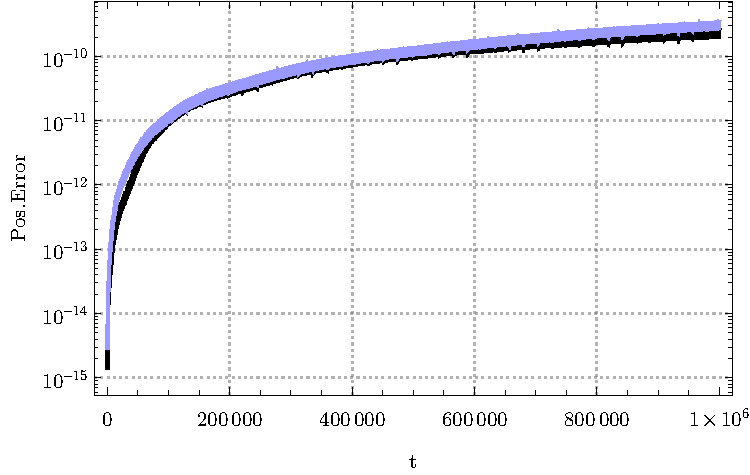
\includegraphics[width=.500\textwidth]{plot6b}
}
\caption{\small N-body: left figure mean energy error evolution $\bar{\triangle E_i}$ and right figure mean Global error evolution $\bar{Ge_i}$ of the 100 integrations for Ideal Integrator (black) and Double prec(blue).}
\label{fig:nbody1}
\end{figure}

\begin{figure}[h]
\centering
\subfloat[Estimation.]{
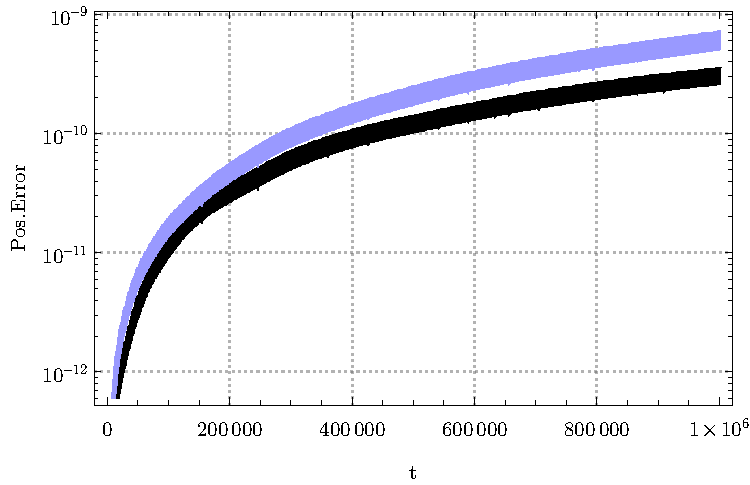
\includegraphics[width=.500\textwidth]{plot7a}
}
\subfloat[Quatlity.]{
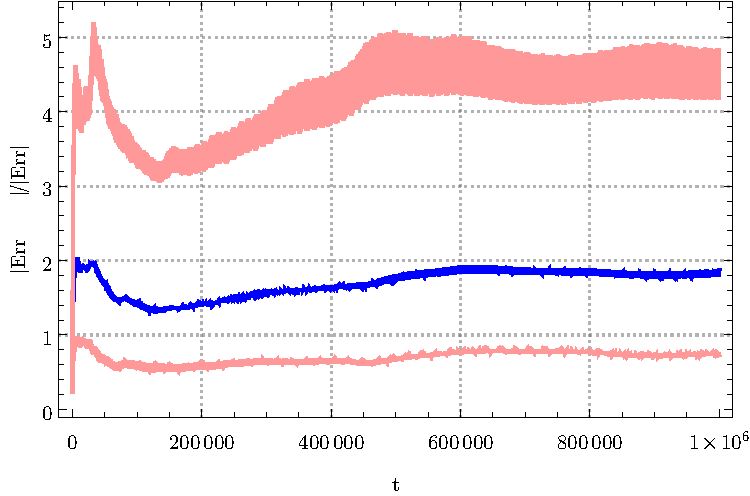
\includegraphics[width=.500\textwidth]{plot7b}
}
\caption{\small Left estimation round-off error, we compare evolution of our estimation error (blue) with evolution of global error (black). Right estimation Quality ,we show mean (blue) and  standard deviation (red) of the quality according our definition of (\ref{eq:eq_Qi}). We use rdigits1=0 and rdigits2=3.}
\label{fig:nbody2}
\end{figure}



\chapter{IRK: Newton.}

\section{Sarrera.}



\chapter{IRK: Eguzki-sistema.}

\section{Sarrera.}

\section{Meta-Algoritmoa.}

Demagun Hamiltondar banagarria,

\begin{equation*}
H(y)=H_A(y)+H_B(y),
\end{equation*}
non $H_A \gg H_B$. 

\paragraph*{}Hau izanik dagokion hasierako problema orokorra,

\begin{equation*}
\dot{y}=J^{-1}\triangledown H(y)=f(y) , \ \ y(t_0)=y_0.
\end{equation*}

\paragraph*{}$f(y)$ eredua, eredu sinple $k(y)=J^{-1}\triangledown H_A(y)$ eta eredu konplexu $g(y)=J^{-1}\triangledown H_B(y)$ baten arteko batura gisa deskonposatu daiteke,

\begin{equation*}
\dot{y}=f(y)=k(y)+g(y).
\end{equation*} 


\paragraph*{} \textbf{Adibidea}.

N-gorputzen problemaren Hamiltondarra, alde Kepleriarra eta planeten interakzioen batura gisa bana daiteke,

\begin{equation*}
H(q,p)=H_k+H_I, \ \ H_k \gg H_I.
\end{equation*}  

\begin{equation}
H_k(q,p)=\frac{1}{2} \sum\limits_{i=0}^{N} \frac{p_i^2}{m_i}- Gm_0 \sum\limits_{i=1}^{N} \frac{m_i}{\|q_i-q_0\|}
\end{equation}

\begin{equation}
H_I(q)=\sum\limits_{1\leq i < j \leq N}^{N} \frac{G \ m_i m_j}{\|q_j-q_i\|}
\end{equation}

\paragraph*{}Banaketa honi dagokion ekuazio diferentzialak,  $f(y)=k(y)+g(y)$ modu honetan laburtuko ditugu. Honako notazioa erabiliz,
\begin{equation*}
\dot{y}=f(y)=
\left(\begin{array}{c}
  \dot{q} \\
  \dot{v} \\
\end{array}\right)=
\left(\begin{array}{c}
  f_q(y) \\
  f_v(y) \\
\end{array}\right)=
\left(\begin{array}{c}
  k_q(y) \\
  k_v(y) \\
\end{array}\right)+
\left(\begin{array}{c}
  g_q(y) \\
  g_v(y) \\
\end{array}\right)
\end{equation*}

\paragraph*{}Batetik, $f_q(y)$ ekuazio diferentzialen deskonposaketa honakoa da,

\begin{align*}
\dot{q}=f_q(y)=v_i,  \ i=0,\dots,N. 
\end{align*}

\begin{align}
\dot{q}=f_q(y) \ \Rightarrow \ \ 
\left \{ \begin{array}{c}
  k_q(y) =v_i, \ \ i=0,\dots,N. \\[.25cm]
  g_q(y) =0,\ \ i=0,\dots,N.\\
\end{array} \right.  
\end{align}

\paragraph*{}Bestetik, $f_v(y)$ ekuazio diferentzialen deskonposaketa honakoa da,

\begin{align*}
\dot{v}=f_v(y)=\sum_{j=0,j \neq i}^{N} \frac{Gm_j}{\|q_j-q_i\|^3} (q_j-q_i) \ \  \ i=0,\dots,N.
\end{align*}

\begin{align}
\dot{v}=f_v(y) \ \ \Rightarrow \ \ 
\left \{ \begin{array}{c}
  k_v(y)=\left \{ \begin{array}{c}
           \dot{v}_0 =\sum_{j=1,j \neq i}^{N} \frac{Gm_j}{\|q_j-q_0\|^3} (q_j-q_0). \\[.30cm]
           \dot{v}_i = \frac{Gm_0}{\|q_0-q_i\|^3} (q_0-q_i), \ \  i=1,\dots,N.\\[.30cm]
         \end{array} \right. \\[.30cm]  
  g_v(y)=\left \{ \begin{array}{c}
             \dot{v}_0=0. \\[.30cm]
             \dot{v}_i= \sum_{j=1,j \neq i}^{N} \frac{Gm_j}{\|q_j-q_i\|^3} (q_j-q_i), \ \  i=1,\dots,N.\\[.30cm]  
           \end{array} \right. \\ 
\end{array} \right.  
\end{align}


\subsection*{Meta-algoritmoa.}

IRK metodoaren formulazioa gogoratuz,


\begin{equation*}
\label{eq:62}
Y_{n,i}=y_n+ \sum\limits_{j=1}^{s} \mu_{ij} L_{n,j}, \ \ L_{n,i}=hb_if(Y_{n,i})
\end{equation*}
\begin{equation*}
\label{eq:63}
y_{n+1}=y_n+\sum\limits_{i=1}^{s} L_{n,i}
\end{equation*}

s-ataleko IRK metodoaren iterazio bakoitzean, ($s*d$) ezezagunetako ($Y_i$) ekuazio-sistema askatu behar dugu: 

\begin{equation*}
Y_{i}-y_n- \sum\limits_{j=1}^{s} \mu_{ij} \ hb_j \bigg(k(Y_{j})+g(Y_{j})\bigg)=0, \ \ i=1,\dots,s.
\end{equation*}

Gure planteamenduan ekuazio-sistema Newton-sinplifikatuaren bidez askatuko dugu, baina jakobiarraren kalkulurik gabe. Lortzen dugun metodoa, jakobiarraren hurbilpena alde kepleriarra kontsideratzen duen ($J=k'(Y_i)$) Newton-sinplifikatuaren baliokidea da. 

\subsubsection*{Garapena.}

\paragraph*{}Ekuazio-sisteman Newton metodoa aplikatuz. Soluziotik gertu dagoen balio batetik abiatuta, ($Y_i^{[0]}$) eta $k=1,2,\dots$, 
\begin{equation*}
\triangle Y^{[k]}=-\frac{F(Y^{[k]})}{F'(Y^{[k]})},
\end{equation*}

\begin{equation*}
Y^{[k+1]}=Y^{[k]}+\triangle Y^{[k]}.
\end{equation*}

IRK metodoaren ekuazio-sistemari aplikatuz,

\begin{equation*}
\triangle Y_i^{[k]}=-\frac{\big(Y_{i}^{[k]}-y_n- \sum\limits_{j=1}^{s} \mu_{ij} \ hb_j                               \big(k(Y_{j}^{[k]})+g(Y_{j}^{[k]})\big)\big)}
                          {\big(1-\sum\limits_{j=1}^{s} \mu_{ij} \ hb_j \big(k'(Y_{j}^{[k]})+g'(Y_{j}^{[k]})\big)\big)}
\end{equation*}

Ekuazio laburtzeko $\delta_i^{[k]}$ aldagai laguntzailea erabiliz hau da askatu beharreko ekuazio,

\begin{equation}
\triangle Y_i^{[k]}=\sum\limits_{j=1}^{s} \mu_{ij} \ hb_j \big(k'(Y_{j}^{[k]})+g'(Y_{j}^{[k]})\big)\triangle Y_j^{[k]}+\delta_i^{[k]},
\end{equation}

non,
\begin{equation*}
\delta_i^{[k]}=-Y_{i}^{[k]}+y_n+ \sum\limits_{j=1}^{s} \mu_{ij} \ hb_j \big(k(Y_{j}^{[k]})+g(Y_{j}^{[k]})\big).
\end{equation*}

Lortutako espresioa garatuko dugu.

\begin{enumerate}
\item \textbf{Lehen hurbilpena.}

$g'(Y_{j}^{[k]}) << k'(Y_{j}^{[k]})$  eta $g'(Y_{j}^{[k]})<\triangle Y_{j}^{[k]}$ denez,
\begin{equation}
\triangle Y_i^{[k]} \approx \sum\limits_{j=1}^{s} \mu_{ij} \ hb_j \ k'(Y_{j}^{[k]}) \ \triangle Y_j^{[k]}+\delta_i^{[k]}
\end{equation}  

\item \textbf{Bigarren hurbilpena (Linealizazioa).}

\begin{equation*}
k(Y_{j}^{[k+1]})=k'(Y_{j}^{[k]}) (Y_{j}^{[k+1]}-Y_{j}^{[k]})+k(Y_{j}^{[k]})+O(\|\triangle Y_j^{[k]}\|^2)
\end{equation*}
\begin{equation*}
\triangle Y_j^{[k]}=Y_j^{[k+1]}-Y_j^{[k]}
\end{equation*}

Honako hurbilpena,
\begin{equation*}
k'(Y_j^{[k]}) \triangle Y_j{[k]} \approx k(Y_j^{[k]}+\triangle Y_j^{[k]})- k(Y_j^{[k]})
\end{equation*}

ordezkatuz eta garatuz,
\begin{equation*}
\triangle Y_i^{[k]}=\sum\limits_{j=1}^{s} \mu_{ij} \ hb_j \ k(Y_j^{[k]}+\triangle Y_j^{[k]})\ -\sum\limits_{j=1}^{s} \mu_{ij} \ hb_j \ k(Y_j^{[k]}) +\delta_i^{[k]},
\end{equation*}

\begin{equation}
\triangle Y_i^{[k]}=-Y_i^{[k]}+y_n+ \sum\limits_{j=1}^{s} \mu_{ij} \ hb_j \ k(Y_j^{[k]}+\triangle Y_j^{[k]})\  +\sum\limits_{j=1}^{s} \mu_{ij} \ hb_j \ g(Y_{j}^{[k]}).
\end{equation}

\item \textbf{Ekuazioak berridatiziz.}

$\triangle Y_i^{[k]}=Y_i^{[k+1]}-Y_i^{[k]}$ definizioa erabiliaz,

\begin{equation}
Y_i^{[k+1]}=y_n+ \sum\limits_{j=1}^{s} \mu_{ij} \ hb_j \ k(Y_j^{[k+1]})\  +\sum\limits_{j=1}^{s} \mu_{ij} \ hb_j \ g(Y_{j}^{[k]}).
\end{equation}
\end{enumerate}


\subsubsection*{Meta-Algoritmoa.}
IRK metodoa aplikatzeko meta algoritmoa planteatuko dugu.

\begin{algorithm}[H]
 \BlankLine
  $e=0$\;
  \For{$n\leftarrow 1$ \KwTo $endstep$}
  {
   \BlankLine
   Hasieratu  $Y_{i}^{[0]} \ \ , \ \ i=1,\dots,s $\;   
   \BlankLine
   $k=1 $\;
   $g_{i}^{[0]}=\sum\limits_{j=1}^{s} \mu_{ij} \ hb_j \ g(Y_{j}^{[0]}) $\;
   Askatu $Y_i^{[k]}=y_{n-1}+ \sum\limits_{j=1}^{s} \mu_{ij} \ hb_j \ k(Y_{j}^{[k]}) \ +g_{i}^{[k-1]} $\;
   \While{ (konbergentzia lortu)}
   {
    \BlankLine 
    $k=k+1$\;
    $g_{i}^{[k-1]}=\sum\limits_{j=1}^{s} \mu_{ij} \ hb_j \ g(Y_{j}^{[k-1]}) $\;
    Askatu $Y_i^{[k]}=y_{n-1}+ \sum\limits_{j=1}^{s} \mu_{ij} \ hb_j \ k(Y_{j}^{[k]}) \ +g_{i}^{[k-1]} $\;
   }
   \BlankLine
    $L_i= hb_i f(Y_i^{[k-1]})$\;
    $\delta_{n}= \sum\limits_{i=1}^{s} L_{i}+e $\;
    $y_{n}=y_{n-1}+ \delta_{n} $\;
    $e=(y_{n-1}-y_n)+\delta_n$\;
   \BlankLine
 }
 \caption{Main Algorithm}
\end{algorithm}

\paragraph*{} Meta-algoritmoari buruzko hainbat ohar:

\begin{enumerate}
\item Barne iterazioak.

Kanpo iterazioa Newton metodoa aplikatuz zehaztu dugu. Barne iterazio aldiz, aukera ezberdinak ditugu.

\paragraph*{} \textbf{Barne-interazioa} puntu finkoaren bidez:

\begin{algorithm}[H]
 \BlankLine
  $l=0$\;
  $Y_i^{[k,0]}=Y_i^{[k-1]}$\;
  \While{ (konbergentzia lortu)}
  {
   \BlankLine
   $l=l+1$\;  
   \BlankLine
   $K_i^{[k,l]}=k(Y_{j}^{[k,l-1]})$\;
   $Y_i^{[k,l]}=y_{n-1}+ \sum\limits_{j=1}^{s} \mu_{ij} \ hb_j \ K_j^{[k,l]} \ +g_{i}^{[k-1]} $\;
  }
 \caption{Main Algorithm}
\end{algorithm}


\item Problema independenteak.

Era honetako deskonposaketa bat dugunean,

\begin{align*}
f\left ( \begin{array}{c}
   y_1 \\
   y_2 \\
\end{array} \right)=
\left ( \begin{array}{c}
   f_1(y_1) \\
   f_2(y_2) \\
\end{array} \right)+
\left ( \begin{array}{c}
   g_1(y_1,y_2) \\
   g_2(y_1,y_2) \\
\end{array} \right),
\end{align*}

eredu sinplifikatua problema independenteak osatzen dituzte eta barne iterazioak modu independentean kalkula daitezke. N-gorputzen eguzki-sistemaren adibidean, eredu sinplifikatua $k(y)$ (eguzkiarekiko interakzioa) planeta bakoitzarentzat problema independentea dugu. Kasu honetan urrats bat finkatuta, kanpo planeten $k(y)$ problema barruko planeta baino azkarrago konbergituko du. 

\end{enumerate}


\subsubsection*{Orokorpena.}

Aurreko atalean, maila bakarreko ereduen deskonposaketa aztertu dugu. Ideia orokortuz, eredu deskonposaketa maila ezberdinetan egin daiteke. Problema bat emanda $\dot{y} =f(y)$, 

\begin{align}
\mbox{1. maila} \ \
\left \{ \begin{array}{c}
  \mbox{Eredu osoa.   } f(y) \\[.25cm]
  \mbox{Eredu sinplea.    } \tilde{f}(y)  \\
\end{array} \right.
\ \Rightarrow \ \
f =\tilde{f}+(f-\tilde{f})  
\end{align}

\begin{align}
\mbox{2. maila} \ \
\left \{ \begin{array}{c}
  \mbox{Eredu osoa.   }\tilde{f}(y) \\[.25cm]
  \mbox{Eredu sinplea.    }\tilde{\tilde{f}}(y)  \\
\end{array} \right.
\ \Rightarrow \ \
\tilde{f} =\tilde{\tilde{f}}+({\tilde{f}}-\tilde{\tilde{f}})  
\end{align}

\paragraph*{} \textbf{Adibidea.}

Demagun ekuazio diferentzialak, $m$ perturbazio funtzio dituela,

\begin{equation*}
\dot{y}=f(y)=k(y)+g1(y)+g2(y)+\dots+gm(y)
\end{equation*}

non $k(y)<<gl(y)$,  $l=1,\dots,m$.

\paragraph*{}$m=2$ deneko kasu partikulara aztertuko dugu,
\begin{equation*}
\dot{y}=f(y)=k(y)+g1(y)+g2(y).
\end{equation*} 

\begin{algorithm}[H]
 \BlankLine
  \textbf{Askatu} $Y_i=y_{n-1}+ \sum\limits_{j=1}^{s} \mu_{ij} \ hb_j \ (k(Y_{j})+g1(Y_{j})+g2(Y_{j})) $\;
 \BlankLine
   \While{ (konbergentzia lortu)}
   {
    \BlankLine 
    $k=k+1$\;
    $g2_{i}^{[k-1]}=\sum\limits_{j=1}^{s} \mu_{ij} \ hb_j \ g2(Y_{j}^{[k-1]}) $\;
    \textbf{Askatu} $Y_i^{[k]}=y_{n-1}+ \sum\limits_{j=1}^{s} \mu_{ij} \ hb_j \ (k(Y_{j}^{[k]})+g1(Y_{j}^{[k]})) \ +g2_{i}^{[k-1]} $\;
    \While{ (konbergentzia lortu)}
       {
        \BlankLine 
         $l=l+1$\;
         $g1_{i}^{[k,l-1]}=\sum\limits_{j=1}^{s} \mu_{ij} \ hb_j \ g1(Y_{j}^{[k,l-1]}) $\;
         \textbf{Askatu} $Y_i^{[k,l]}=y_{n-1}+ \sum\limits_{j=1}^{s} \mu_{ij} \ hb_j \ k(Y_{j}^{[k,l]})+g1_{i}^{[k,l-1]} \ +g2_{i}^{[k-1]} $\;
       }
   }
   \BlankLine

 \caption{Main Algorithm}
\end{algorithm}

\paragraph*{}Erlatibitate efektua gehitzerakoan, N-gorputzen problemari dagokion ekuazio diferentziala,

\begin{equation*}
\dot{y}=f(y), \ f(y)=k(y)+g(y)+rs(y)+rn(y),
\end{equation*}

\begin{lstlisting}
k(y): kepleriarra.
g(y): planeten arteko grabitazio interakzioak.
rs(y): eguzkiarekiko erlatibitate efektua.
rn(y): planeten arteko erlatibitate efektuak.
\end{lstlisting}

\subsubsection*{Adierazpena.}

Ekuazio diferentzialen deskonposaketak, zuhaitz moduan adieraz daitezke.

\begin{equation*}
\dot{y}=f(y).
\end{equation*}

\begin{tikzpicture}[scale=.8]
%\draw (-1,-2) grid (5,2);
\filldraw[black] (0,0) circle (2pt);
\end{tikzpicture}

\begin{equation*}
f\left ( \begin{array}{c}
   y_1 \\
   y_2 \\
\end{array} \right)=
\left ( \begin{array}{c}
   f_1(y_1) \\
   f_2(y_2) \\
\end{array} \right)+
\left ( \begin{array}{c}
   g(y) \\
\end{array} \right),
\end{equation*}

\begin{tikzpicture}[scale=.8]
%\draw (-1,-2) grid (5,2);
\filldraw[black] (0,0) circle (2pt);
\filldraw[black] (1,2) circle (2pt);
\filldraw[black] (-1,2) circle (2pt);
\draw (0,0) -- (1,2);
\draw (0,0) -- (-1,2);
\end{tikzpicture}

\begin{equation*}
f_1\left ( \begin{array}{c}
   y_1 \\
\end{array} \right)=
\left ( \begin{array}{c}
   f_{11}(y_{11}) \\
   f_{12}(y_{11},y_{12}) \\
   f_{13}(y_{11},y_{12},y_{13}) \\
\end{array} \right)+
\left ( \begin{array}{c}
   g_1(y_1) \\
\end{array} \right),
\end{equation*}


\begin{tikzpicture}[scale=.8]
%\draw (-1,-2) grid (5,2);
\filldraw[black] (0,0) circle (2pt);
\filldraw[black] (1,2) circle (2pt);
\filldraw[black] (-1,2) circle (2pt);
\filldraw[black] (-2,4) circle (2pt);
\filldraw[black] (-1,4) circle (2pt);
\filldraw[black] (0,4) circle (2pt);
\draw (0,0) -- (1,2);
\draw (0,0) -- (-1,2);
\draw (-1,2) -- (-2,4);
\draw (-1,2) -- (-1,4);
\draw (-1,2) -- (0,4);
\end{tikzpicture}

\part{synthesys}
\chapter{Eranskinak}.

\section{Kepler ekuazioak eta definizioak.}

\paragraph*{\textbf{Kepler ekuazioak (definizioa)}},
\begin{equation*}
E_0-e\sin E_0=n (t_0-t_p)
\end{equation*}
\begin{equation*}
E_1-e\sin E_1=n (t_1-t_p)
\end{equation*}
non $n=\frac{2\pi}{P}$, $P$ periodoa den.

\paragraph*{} Honako garapen hau egingo dugu,
\begin{equation*}
E_1-E_0-e(\sin(E_1)-\sin(E_0))=n \triangle t \ \ \ \longrightarrow \ \triangle E - e(\sin(E_0+\triangle E)-\sin(E_0))=n \triangle t
\end{equation*}
\begin{equation*}
E_1=E_0+\triangle E  
\end{equation*}

\begin{equation*}
\triangle E - ce \ \sin(\triangle E- se \ (\cos(\triangle E)-1)=n \triangle t
\end{equation*}
non, $ce=e \ \cos(E_0)$ eta $se=e \ \sin(E_0)$

\paragraph*{\textbf{Newton metodoa}},
\begin{equation*}
f(\triangle E)=\triangle E - ce \sin(\triangle E)- se (\cos(\triangle E)-1)-n \triangle t=0
\end{equation*}
\begin{equation*}
f'(\triangle E)=1-ce \cos(\triangle E)+ se \sin(\triangle E)
\end{equation*}
\begin{equation}
\triangle E^{[k+1]}=\triangle E^{[k]}- \frac{f(\triangle E^{[k]})}{f'(\triangle E^{[k]})}
\end{equation}

\paragraph*{\textbf{$\triangle E^{[0]}$ hasierako balioa}}, finkatzea da dugun zailtasun handiena. Horretarako honako garapena egingo dugu,
\begin{equation*}
\triangle E - ce \ \sin(\triangle E- se \ (\cos(\triangle E)-1)=n \triangle t
\end{equation*} 
\begin{equation*}
x=\triangle E- n \triangle t
\end{equation*}

eta beraz,
\begin{equation*}
x-ce \sin(n\triangle t+x)-se(cos(n \triangle t+x)-1)=0
\end{equation*}

Honako baliokidetasun trigonometrikoak aplikatuz,
\begin{equation*}
\cos(A+B)=\cos(A)\cos(B)-\sin(A)\cos(B)
\end{equation*}
\begin{equation*}
\sin(A+b)=\cos(A)\sin(B)+\sin(A)\cos(B)
\end{equation*}

berdintza hau lortzen dugu,
\begin{equation*}
x- (se \ \cos(n \triangle t)+ ce \ \sin(n \triangle t)) \cos(x)+ (se \ \sin(n \triangle t)-ce \ \cos(n \triangle t)) \sin(x)+se =0
\end{equation*}

$x$ txikia denean honako hurbilpenak ordezkatuz,
\begin{equation*}
x \approx \sin(x), \ \cos(x) \approx 1- \frac{x^2}{2}
\end{equation*}
\begin{equation}
(se \ \cos(n \triangle t)+ce \ \sin(n \triangle t)) \frac{x^2}{2}+ (1+se \ \sin(n \triangle t)-ce \cos(n \triangle t))x-(se )=0
\end{equation}

Goiko ekuazio hau askatuz ($Ax^2+Bx+C=0, \ \rightarrow x=\frac{-B\pm \sqrt{B^2-4AC}}{2A}$) lortuko dugu $\triangle E^{[0]}=x+n\triangle t$.

\paragraph*{\textbf{Koordenatu kartesiarren}}, kalkulua modu ekuazio hauen bidez egingo dugu,

\begin{equation*}
(q_1,v_1)=(q_0,v_0)+ (q_0,v_0) \left(\begin{array}{cc}
                                       b_{11} & b_{12} \\
                                       b_{21} & b_{22} \\
                                \end{array}\right)
\end{equation*}

\begin{equation*}
b_{11}=(C-1) \frac{a}{\|q\|}
\end{equation*}

\begin{equation*}
b_{21}=\triangle t+(S-\triangle E) \frac{a^{\frac{3}{2}}}{\mu^{\frac{1}{2}}}
\end{equation*}

\begin{equation*}
b_{12}=\frac{s}{\|q\| \sqrt{a} (1-ce \ C +se \ S)}
\end{equation*}

\begin{equation*}
b_{22}=\frac{C-1}{1-ce \ C+ se \ S}
\end{equation*}

Eta osagai bakoitzaren definizioa,
\begin{equation*}
C=\cos(\triangle E), \ S=\sin(\triangle E)
\end{equation*}

\begin{equation*}
ce=e \ \cos(E_0) = \|q\| \|v\|^2-1
\end{equation*}

\begin{equation*}
se= e \ \sin(E_0)=\frac{(q \cdot v)}{\sqrt{\mu \ a}}
\end{equation*}

\begin{equation*}
a= \frac{\mu \|q\|}{2\mu-\|q\|\|v\|^2}
\end{equation*}

\begin{equation*}
n= \frac{\mu^{\frac{1}{2}}}{a^{\frac{3}{2}}}
\end{equation*}

\paragraph*{\textbf{Biribiltze errorea}}. $\triangle E$ txikia denean, $\cos(\triangle E)-1$ espresioaren kalkuluaren ezabapen arazoak biribiltze errore handia eragin dezake. Hori konpontzeko baliokidetasun hau erabiliko dugu,

\begin{equation*}
\cos(\triangle E)-1=-\frac{(\sin^2(\triangle E)}{1+\cos(\triangle E)}
\end{equation*}  

Eta beraz, kepler-en ekuazioak hauek izango dira,
\begin{equation*}
f(\triangle E)=\triangle E - ce \sin(\triangle E)+ se \bigg(\frac{(\sin^2(\triangle E)}{1+\cos(\triangle E)}\bigg)-n \triangle t=0
\end{equation*}

Eta $(q_1,v_1)$ balioak kalkulatzeko,

\begin{equation*}
b_{11}=(C-1) \frac{a}{\|q\|}, \longrightarrow b_{11}=-\frac{(\sin^2(\triangle E)}{1+\cos(\triangle E)} \frac{a}{\|q\|}
\end{equation*}

   

%\include{Appendix}

%\begin{acknowledgements}
%If you'd like to thank anyone, place your comments here
%and remove the percent signs.
%\end{acknowledgements}
\nocite{*}
\bibliography{./bibliografia/mybib}
\bibliographystyle{myplain2-doi}

\end{document}


